\section{Introduction}
\todo{rename patient to bci user and participant}

BCIs for communication assistive technology~\cite{Millan2010}
have a target population consisting of patients people with \ac{sspi}.

Yet, there is a large comorbidity between \ac{sspi}, and eye motor impairment~\cite{FriedOken2020}.
Impairments such as nystagmus (uncontrolled eye movements), diplopia (double
vision), and ophthalmoplegia (eye paralysis) can significantly hinder
the ability to use visual BCIs. These impairments make it difficult for
individuals to focus on or track visual stimuli accurately, reducing their
performance with BCIs that rely on visual cues~\cite{McCane2014,FriedOken2020,Pasqualotto2015}.
Unfortunately, it is again for this group that eye tracking solutions also
perform poorly, making them more reliant on potential developments in \ac{bci}
that do not rely on eye gaze.

Eye motor impairments are presumed to reduce performance in operating visual
oddball \ac{bci}s (see section\todo{ref section} for an overview), since users
cannot comfortably redirect their gaze at the desired target,
i.e., perform overt \ac{vsa}.
This is usually circumvented by designing gaze-independent~
\acp{bci}~\cite{Riccio2012}.
These interfaces either avoid visual stimulation, or exploit some form of
covert \ac{vsa}, where the gaze and \ac{vsa} do not coincide.

Several studies with visual oddball \acp{bci} show that performance drops when not fixating the intended
target~\cite{Brunner2010, Treder2010, RonAngevin2019}, necessitating
gaze-independent solutions.
These studies build on the assumption that patients with eye motor impairment
would feel comfortable operating an interface in pure covert \ac{vsa} with
central fixation.
One could argue that a \ac{bci} that is only verified to work when a central
fixation is maintained, could also be considered gaze-dependent.
This does not account for the residual eye motor capabilities of most people
with \ac{sspi}, the (dis)comfort they experience while
performing gaze fixation and other confounding factors due to their eye
motility or vision.

It is a striking constatation that studies reporting on
gaze-independent visual \ac{bci} with people with \ac{sspi} and eye-motor
impaired are very few.
Results are usually different than those obtained with healthy control
participants in the lab, due to difference in capabilities, brain
response, equipment and environment.

\textcite{Lesenfants2014} tested a gaze-independent \ac{ssvep} \ac{bci} in six
participants with \ac{lis} yet only exceeded chance level accuracy in two.
More recently, \textcite{Peters2020} performed a trial with a
interface with two participants with late-stage \ac{als} and visual impairment.
Their system showed high accuracy, outperforming an eye tracking alternative.
It would be of interest to verify if such results can be verified with other
patient groups and visual oddball \acp{bci}.

\textcite{Severens2014} evaluated the visual Hex-o-Spell~\cite{Treder2010} on 5
participants with \ac{als} and showed that this visual oddball interface optimized
for gaze-independence can outperform a tactile gaze-independent \ac{bci}.
While this speaks to the power of visual paradigms even in groups that are
expected to have eye motor impairment, they did not verify the gaze direction
of participants during the experiment.
It was suggested that patients were performing overtly.
Participants with \ac{als} also had a substantially lower accuracy patients lower than healthy
(58\% vs 88\%).


Our previous study, presented in chapter \todo{ref chapter} also used the
visual Hex-o-Spell interface~\cite{VanDenKerchove2024}.
This work partially accounted for the idea that gaze impaired patients might
not full rely on central gaze fixation and evaluates settings that are not
strictly dependent on this.
We showed gaze-independent performance can be improved
improved in healthy subjects using a suited decoding strategy.
that accounts for latency jitter in covert \ac{vsa} responses improves
Yet, there is a strong need for verification of these result in an applied
setting with people with \ac{sspi}.

\todo{discuss \cite{FriedOken2020}}

Eventually, one of the end goals of this research line is to develop
gaze-independent \ac{bci} for peopl that are fully locked-in and have no option left than to use a \ac{bci}.
However, this group is very small and it is often a challenge to recruit them
into a study and perform experiments with them~\cite{Wolpaw2006}.
Patients with less severe paralysis or in less progressed disease stages that struggle with
eye-tracking technology could also benefit from
solutions tailored to their specific situation.
Therefore, we aim to apply the concepts from earlier work an literature to
people with \ac{sspi} and various degrees motor impairment in a visuall oddball
\ac{bci}.
The objectives of this case study are as follows:
\begin{enumerate*}
  \item Explore capabilities and experienced comfort of eye motor impaired
    patients,
  \item evaluate the performance of a gaze-independent visual \ac{bci} in patients
  \item verify if this performance can be improved with a suitable decoding
    strategy.
\end{enumerate*}


\section{Materials \& methods}
\subsection{Patient recruitment}
Patients were recruited from across the Neuromuscular Reference center at
University Hospital Leuven (Leuven, Belgium), TRAINM Neuro Rehab Clinics
(Antwerp, Belgium), the Neurorehabilitation Unit at University Hospital Lille
(Lille, France) and a specialized care home (France).
Experiments were performed under the supervision of their treating physician.
Patients were recruited based on the following criteria.
To qualify for inclusion, patients must
\begin{enumerate}
	\item be at least 18 years old and no older than 60
	years,
  \item belong to class 2 or 3 according the \ac{bci}	patient selection criteria
    presented by~\textcite{Wolpaw2006},\label{item:patients/inclusion/wolpaw}
  \item have limitations to the extent or comfort of their eye motor control\label{item:patients/inclusion/oculomotor}
\end{enumerate}
Patients were excluded if they
\begin{enumerate}
  \item have a diagnosis of a major medical condition, including any major
    neurological or psychiatric disorder other than those of interest based on
    inclusion criteria~\ref{item:patients/inclusion/wolpaw},
    and~\ref{item:patients/inclusion/oculomotor}\label{item:patients/exclusion/medical}
  \item have a predisposition to or have a history of any kind of epileptic seizures,
    including photosensitive epilepsy,\label{item:patients/exclusion/epilepsy}
  \item have a severe loss in vision or hearing, that would significantly impair
        participation in the experiment,\label{item:patients/exclusion/vision}
  \item are currently using specific psychoactive medications or substances that could affect the out-
        come.\label{item:patients/exclusion/cognitive}
  \item be able to understand the experiment instructions and cooperate,
  \item have any other limitations preventing them from performing the given task.
\end{enumerate}

In total, 11 patients were contacted, of which 1 \ac{ms} patient was excluded based on
criterion~\ref{item:patients/exclusion/vision}, 1 \ac{tbi} patient on
both~\ref{item:patients/exclusion/epilepsy}
and~\ref{item:patients/exclusion/cognitive}, and one stroke patient based
on~\ref{item:patients/exclusion/medical}
One further stroke patient was excluded due to technical
difficulties during the experimental session.
Vision was assessed using a LogMAR chart~\cite{Bailey1976}.

Ultimately, 7 patients were retained.
Of these, one patient was diagnosed from bulbar-onset \ac{als}.
\ac{als} is a neurodegenerative disease affecting the motor neurons, leading to
progressive loss of motor function.
This initially results in general weakness and loss of muscle tone, but
eventually results in full body paralysis.\todo{cite}
Although speech and especially eye movements are usually preserved until the
later stages of the disease progression, the bulbar-onset variant is
characterized by an early loss of speech and an increased involvement of eye
motor symptoms~\cite{Guo2022}\todo{which?}.
Furthermore, one of the goals of \ac{bci} is to support \ac{als} patients whose
life span has been extended with life support with and assistive technology to
ensure quality of life.
In these very progressed stages of \ac{als}, eye movement will eventually also
be affected~\cite{Hayashi1991}.

Three other patients were diagnosed with \ac{fa}, a neurodegenerative
disease affecting the
spinal cord, peripheral nervous system and cerebellum.
\ac{fa} results in an impairing loss of muscle coordination.
In progressed stages, the disease can present with nystagmus, saccadic
intrusions and gaze dysmetria~\cite{Cook2017}.

The final three patients were stroke patients.
Brain stem and cerebellar stroke can often lead to forms of \ac{lis}, and
various eye motor disorders are common depending on the exact etiology
~\cite{Bogousslavsky1987, Moncayo2009}.
Stroke can lead to some of the more severe impairments like ophthalmoplegia or
partial ophthalmoplegia immediately from onset.

Table~\ref{tab:patients/patients} lists the included patients and their
diagnoses.

\todo{check Usability and Workload of Access Technology for People With Severe
Motor Impairment: A Comparison of Brain-Computer Interfacing and Eye Tracking}

\begin{table}[t]
  \centering
  \footnotesize
  \begin{tabular}{llllllllr}
  \toprule
  \textbf{ID}  & \textbf{Age} & \textbf{Sex} & \textbf{Hand.} &
  \textbf{Diagnosis}
  & \textbf{Speech}     & \textbf{Trach.} & \textbf{Communication}          &
  \textbf{Cls.} \\ \midrule
  PA1 & 58  & M   & L     & bulbar-onset \acs{als} & anarthric  & no          & tablet                 & 3  \\
  PB1 & 41  & M   & L     & \acs{fa} & dysarthric & no          & verbal                 & 3  \\
  PB2 & 43  & F   & R     & \acs{fa} & dysarthric & no          & verbal                 & 3  \\
  PB4 & 48  & M   & R     & \acs{fa} & dysarthric & no          & verbal                 & 3  \\
  PC2 & 43  & M   & R     & brainstem stroke & anarthric  & yes         & \makecell[l]{prompting\\+eye movement} & 2 \\
  PC3 & 43  & F   & R     & brainstem stroke & anarthric  & yes         & letterboard            & 2 \\
  PC4 & 54  & M   & R     & \makecell[l]{left cerebellar stroke \\ (trombosis of the basilar artery)} & anarthric  & yes & letterboard & 2 \\
  \bottomrule
\end{tabular}

  \caption[Presentation of included patients including their diagnosis and
  capabilities.]{Presentation of included patients including their diagnosis and
  capabilities.
  (Trach.: patient underwent a tracheostomy, Cls.: classification according
  to~\textcite{Wolpaw2006}).
  }
  \label{tab:patients/patients}
\end{table}
\todo{Replace with classification according to 40. Kübler A, Birbaumer N.
Brain-computer interfaces and communication in paralysis: extinction of goal
directed thinking in completely paralysed patients? Clin Neurophysiol.
2008;119:2658-2666.}
\todo{include year of diagnosis}

\subsection{Visual skills and eye tracking and eye motor examination}

Self-reported eye motor and visual abnormalities were recorded according to the
relevant visual \ac{bci} skills presented by~\textcite{FriedOken2020}.
These include visual acuity, visual fixation, eyelid function, ocular motility
, binocuar vision and field of vision.
Additionally, participants were asked about eye tremors (nystagmus or other) and
other involuntary eye movements.

As an objective metric, we implemented and performed the automated NeuroEye eye movement
test proposed by~\textcite{Hassan2022} using calibration-free eye tracking to
check if it revealed any further eye motor abnormalities.
This was not the case.
This test is based on calibration-free eye tracking.
\todo{say which part we used and which part not}
\todo{motivation and text and references Juliette}
\todo{Limited in what it can tell us (check paper)}
\todo{include eye test document juliette}

Table~\ref{tab:patients/eye} details their eye motor impairments and vision of
included patients.
All participants reported some degree of fatigue or discomfort when fixating.
Patient PA1 had the mildest impairment, only reporting fatigue when fixating
for prolonged times.
The \ac{fa} patients were mostly affected by eye tremors and impaired pursuit.
Eye motor function of participants PC2, PC3, and PC3 were most severly affected.
Participant PC2 was only able to look up and down and had a deviation in the
left eye causing diplopia, but this was corrected by a prism glass.
Participant PC3 only retained partial motility of the right eye, while the left eye was permanently closed.
Participant PC4 had one deviated eye with a corneal abcess affecting the motility
and vision in the right eye, and suffered reduced motility in the left.
\todo{go through notes again}

\begin{table}[t]
  \centering
  \footnotesize
  % \begin{tabular}{lll}
%  \toprule
%  \textbf{ID} & \textbf{Oculomotor impairment} & \textbf{Vision (LogMAR)} \\ \midrule
%  PA1  & fixation fatigue & 0.0 \\
%  PB1  & impaired pursuit, fixation fatigue, fixation discomfort, tremor & 0.0 \\
%  PB2  & fixation fatigue, fixation discomfort, tremor & 0.6 \\
%  PB4  & impaired pursuit, fixation fatigue, fixation discomfort, tremor & 0.2 \\
%  PC2  & \makecell[l]{partial ophthalmoplegia (up-down preserved), \\ fixation
%  fatigue, fixation discomfort, tremor} & \makecell[l]{0.0, diplopia corrected \\ with prism glass)} \\
%  PC3  & \makecell[l]{right ophthalmoplegia, left partial ophthalmoplegia, \\ fixation fatigue, fixation discomfort, tremor} & 0.7, right eye closed \\
%  PC4  & deviation of the left eye & 0.6 \\
%  \bottomrule
%\end{tabular}
\footnotesize
\let\oldarraystretch\arraystretch
\renewcommand{\arraystretch}{2}
\newcommand{\skill}{\cellcolor{lightgray}}
\newcommand{\noskill}{\cellcolor{accent1}\textcolor{muteblack}{\BigCross}}
\newcommand{\snoskill}{\cellcolor{accent2}\textcolor{muteblack}{\BigDiamondshape}}
\begin{tabular}{r|ccccccc}
                          & PA1      & PB1      & PB2       & PB4      & PC2       & PC3       & PC4 \\ \hline
  Visual fixation         & \noskill & \noskill & \noskill  & \noskill & \noskill  & \noskill  & \noskill \\
  Eyelid function         & \skill   & \skill   & \skill    & \skill   & \noskill  & \noskill  & \skill \\
  Ocular motility         & \skill   & \noskill & \skill    & \noskill & \snoskill & \snoskill & \noskill\\
  Binocular vision        & \skill   & \skill   & \skill    & \skill   & \noskill  & \snoskill & \snoskill \\
  Field of vision         & \skill   & \skill   & \skill    & \skill   & \skill    & \noskill  & \noskill \\
  Involuntary movement    & \skill   & \noskill & \noskill  & \noskill & \noskill  & \noskill  & \skill \\ \hline
  Visual acuity   & 0.0      & 0.0      & 0.6       & 0.2      & 0.0       & 0.7  & 0.6\\
\end{tabular}

  \caption[Visual skills of the included participants.]{%
  Visual skills of the included participants.
  Visual~\ac{bci} skills~\cite{FriedOken2020}
  was assessed with a combination of self-reported issues
  by the subject and the NeuroEye~\cite{Hassan2022} test. \BigCross\
  impaired, \BigDiamondshape\ severely impaired. Visual acuity in logMAR, lower
  is better.}
  \label{tab:patients/eye}
\end{table}

Finally, we also record gaze position throughout the experimental session, to
register the participant's gaze relative to the stimulated \ac{bci} targets.

\subsection{\Ac{bci} stimulation}

The \ac{bci} stimulation procedure was based on the
Hex-o-Spell~\cite{Treder2010} implementation presented
by~\textcite{VanDenKerchove2024}.
Similar to this study, the task consists of counting the flashes of a cued
target among 6 round, flashing targets laid out in a hexagonal pattern in the
field of view of the user.
We refer to section~\ref{sec:covert-align/stimulation} for implementation details.

3 different \ac{vsa} settings were explored
In overt \ac{vsa}, the participant was instructed to fixate the cued target, or
try to the maximum extent of their visual skill, even if experiencing slight
discomfort.
In covert \ac{vsa}, the participant was instructed to fixate the center of the
screen, also to the extent of their ability.
An additional \emph{free \ac{vsa}} condition was introduced.
Here, the patient was instructed to perform the task as they deemed most
comfortable.
This allows us to investigate the user's natural way of operating the \ac{bci}
given their individual set of visual skills.
If the participant was not fully paralyzed, they were instructed not to move the head.
The cued \emph{split attention} setting proposed
by~\textcite{VanDenKerchove2024} is not studied here, since we are interested
in natural \ac{vsa} operation settings for gaze-impaired individuals.

To make the interface suitable for use by individuals with
\ac{sspi}~\cite{FriedOken2020}, the
number of blocks was decreased to 6 per \ac{vsa} setting.
\Ac{isi} was increased to\todo{number} to decrease task difficulty.
The experiment also started with a training block in each condition, where the
participant was instructed with feedback on their performance to make sure they
understood and were able to perform the task.

\fourpanefig{%
  \figpane{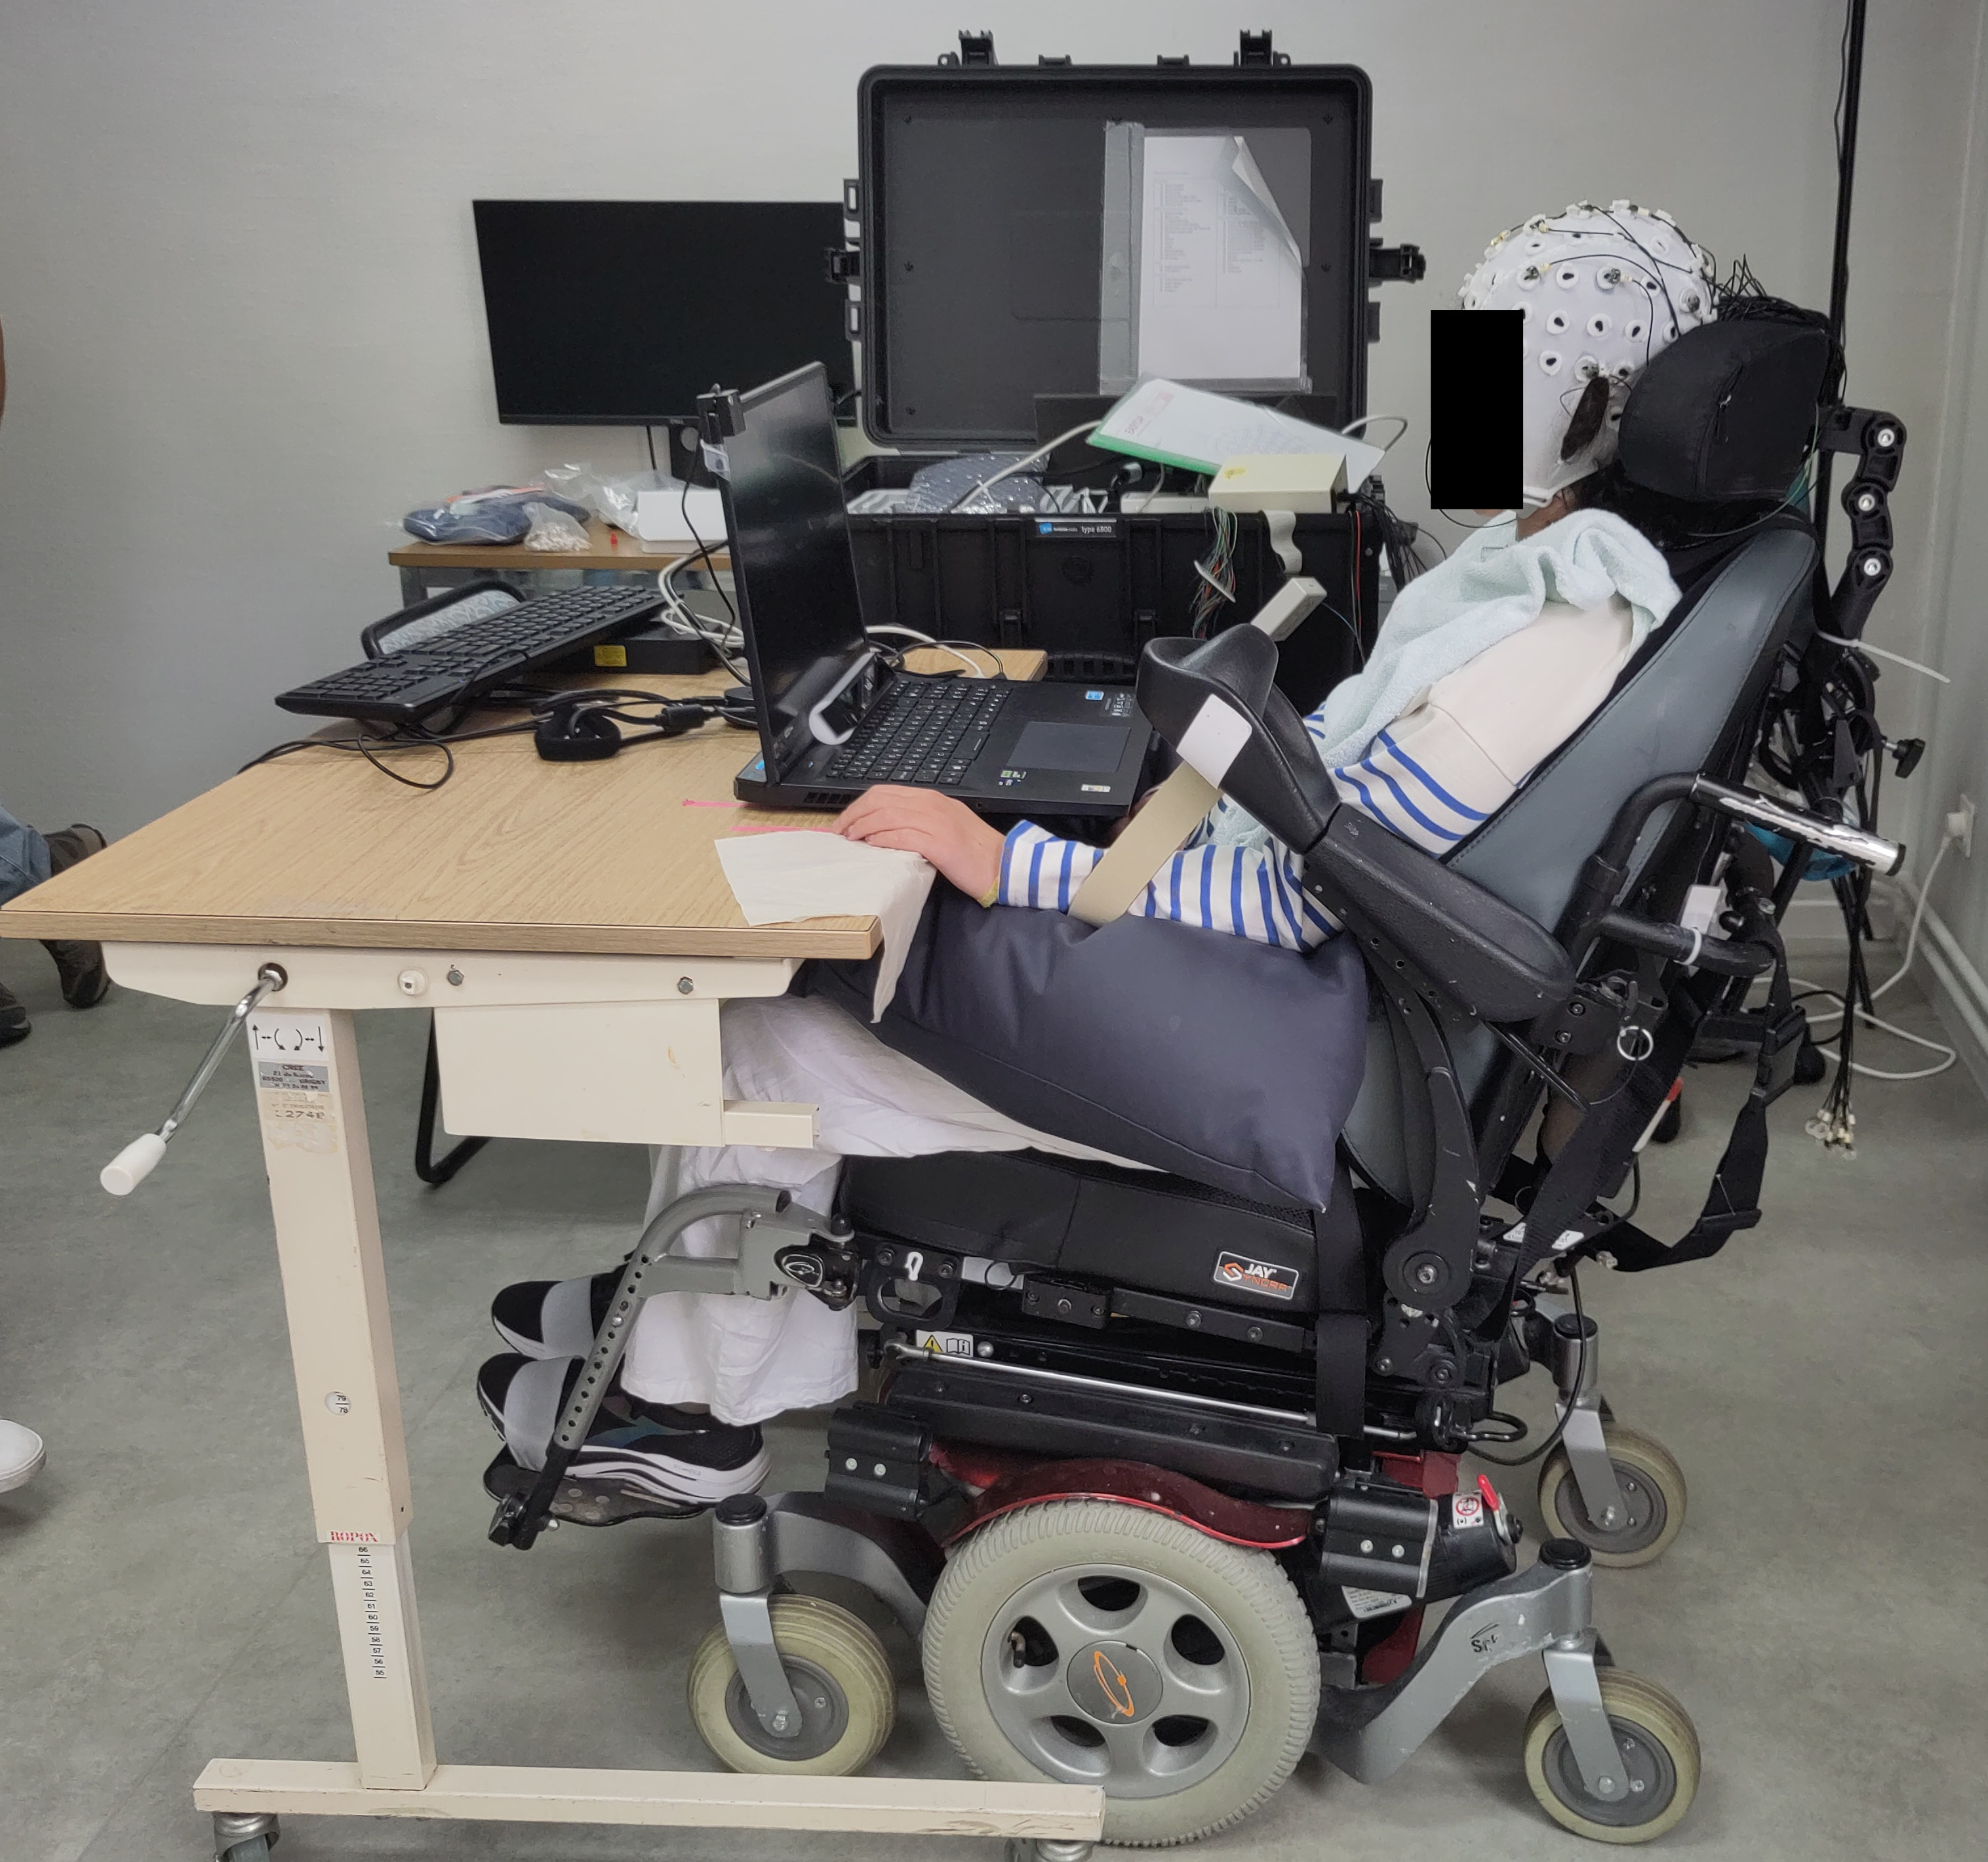
\includegraphics[width=\textwidth]{figures/patients/PD01a-obfuscated.jpg}}{A
  patient with the stimulation and recording setup.}{fig:patients/photos/side}
}{%
  \figpane{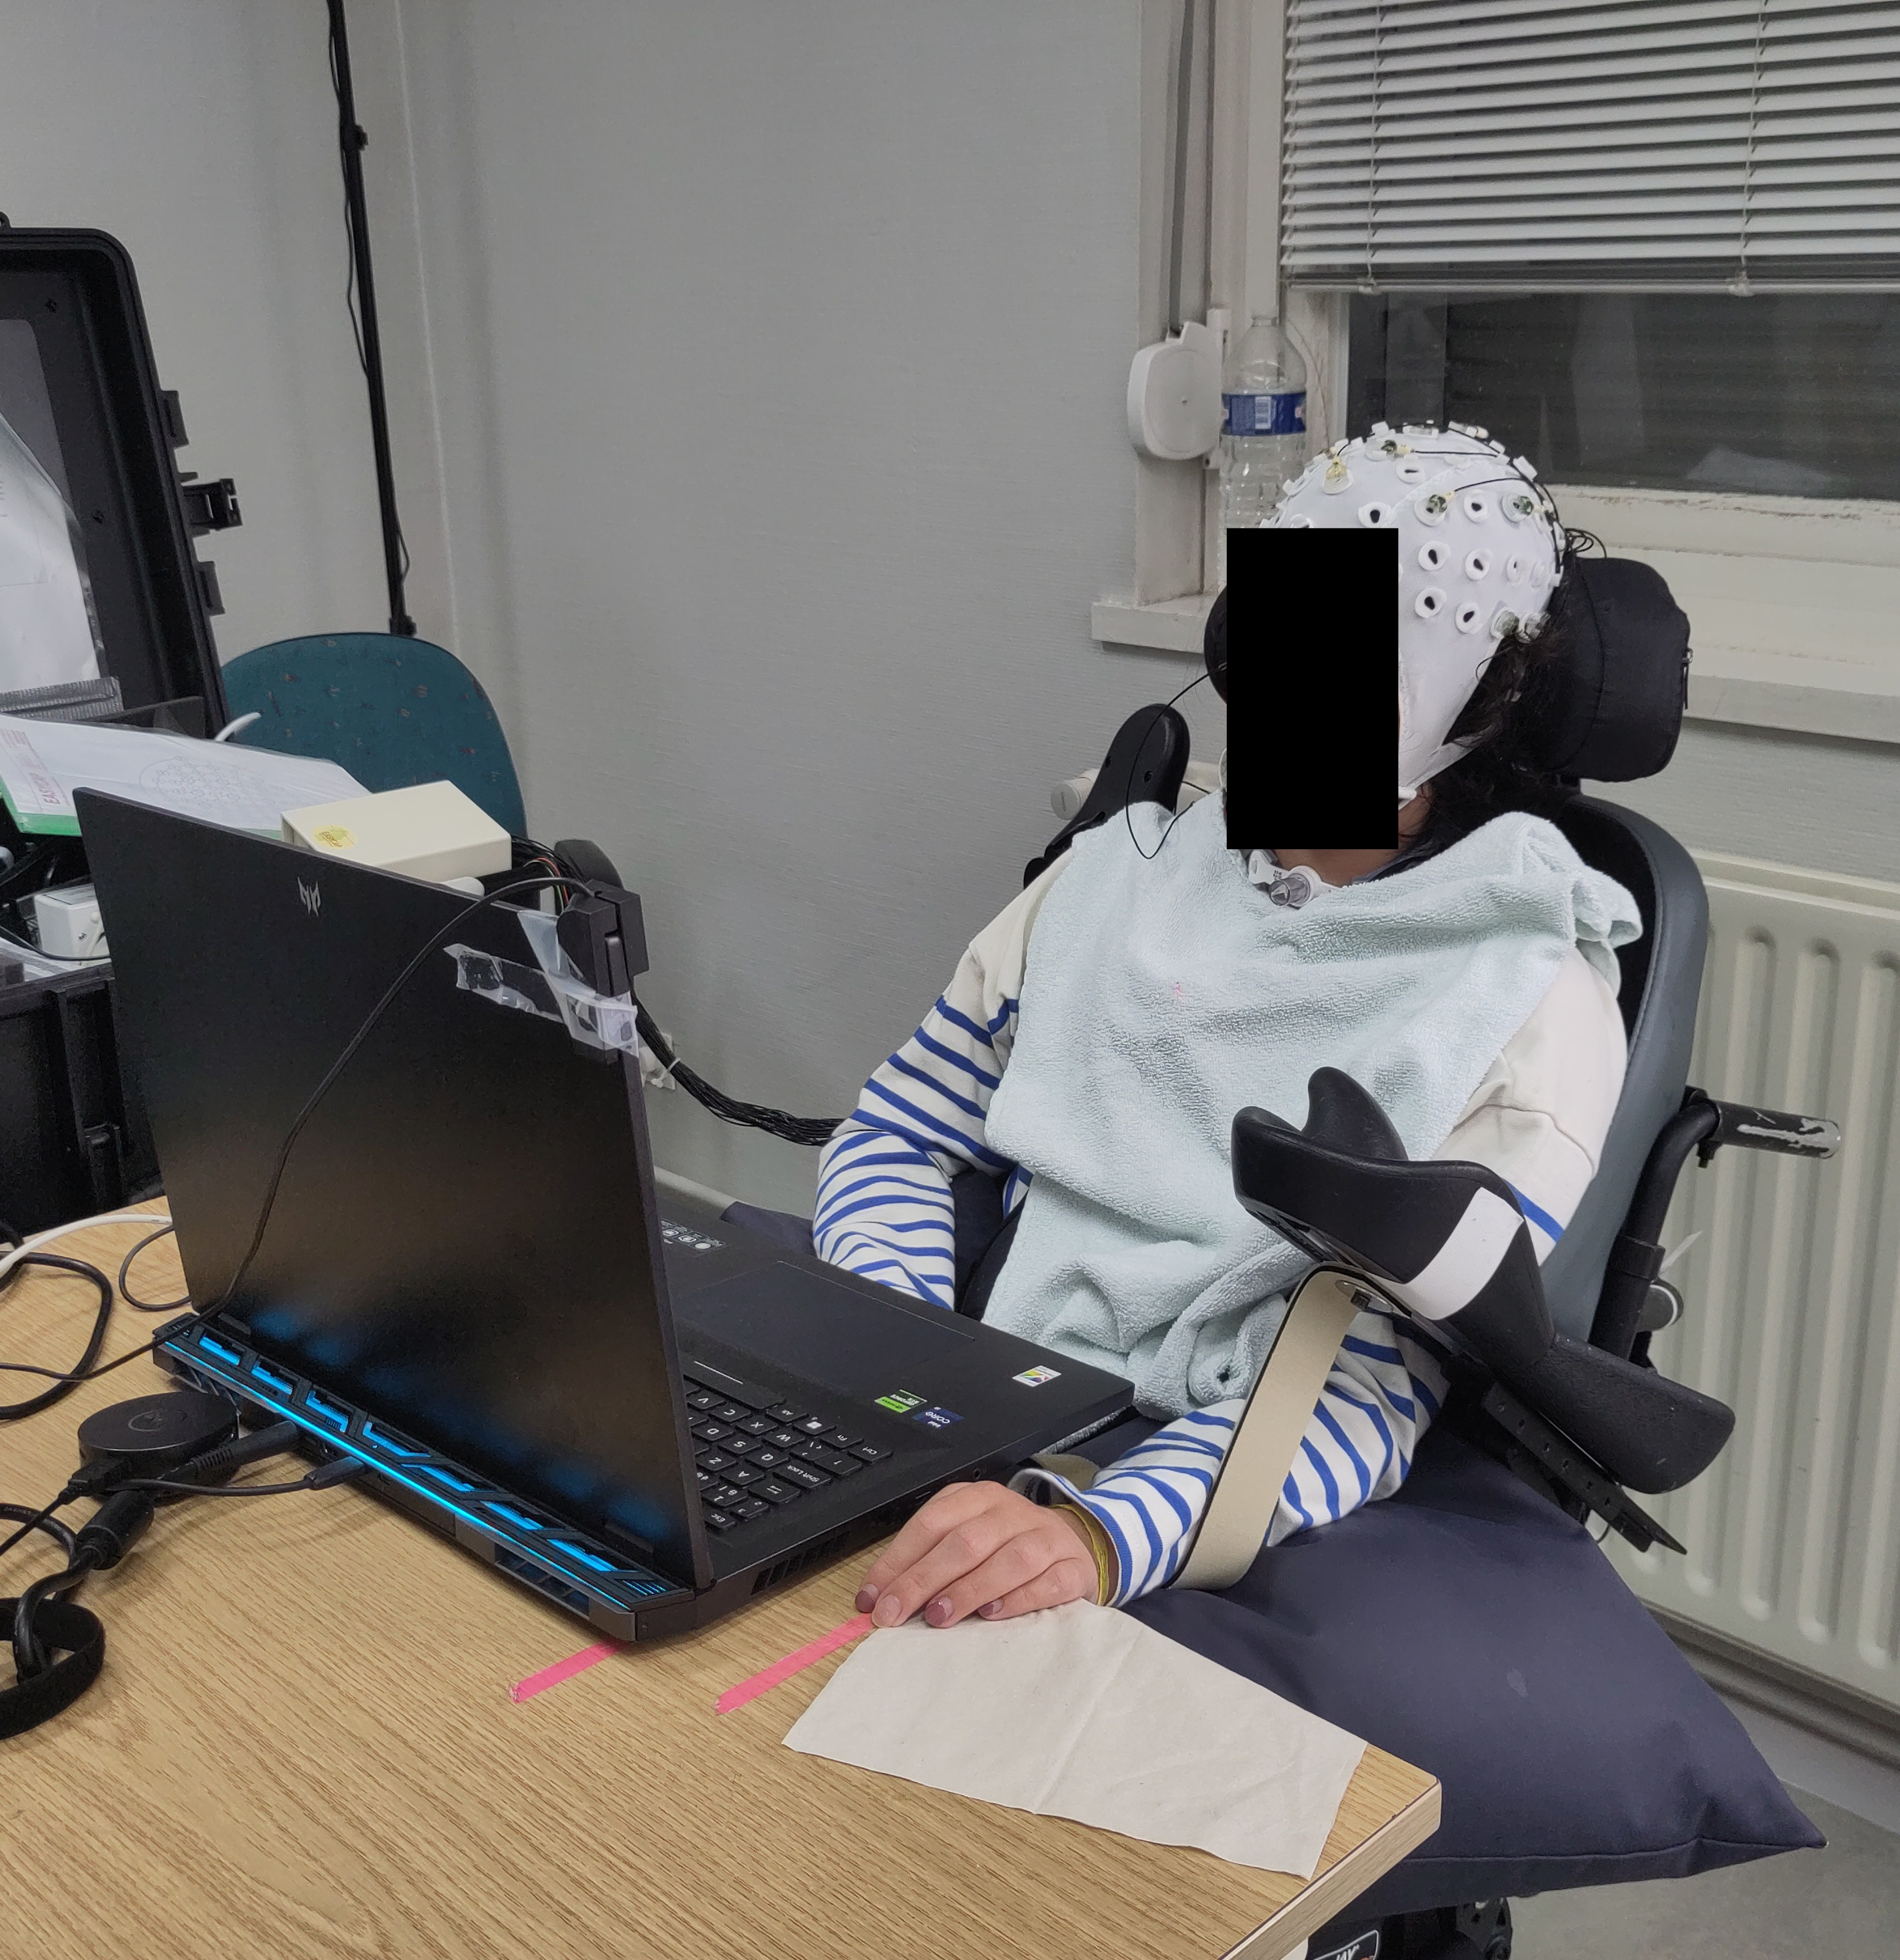
\includegraphics[width=\textwidth]{figures/patients/PD01b-obfuscated.jpg}}{subcaption}{fig:patients/photos/front}
}{%
  the interface
}{%
  4
}{%
  caption
}{fig:patients/photos}

\subsection{Data collection \& preprocessing}

During the recording session, patients were positioned in their wheelchair in front of a table.
Stimuli were presented on a laptop \todo{model, make} placed at \todo{distance}
A Cedrus StimTracker \todo{make} ensured synchronization of stimuli with the
recorded \ac{eeg}.
Eye tracking throughout was performed using the Tobii~\todo{model, make}
portable eye tracker placed at the bottom of the laptop screen.

\Ac{eeg} was recorded at 1000Hz using the Neuroscan Neuvo  portable amplifier (Compumedics Neuroscan,
Australia) connected to a second laptop for registration
The \ac{eeg} headset used 18 active AgCl electrodes (EASYCAP GmbH, Germany) placed on a cap
according to the international 10-20 layout.
Using electrolyte gel, electrode impedances were reduced below 10k$\Omega$
Additionally, the \ac{eog} was recorded.

The \ac{eeg} was band-pass filtered between 0.5 and 16Hz.
Bad channels were rejected using on the RANSAC algorithm~\cite{Fischler1981}
and visual inspection.
Next, the \ac{eeg} was rereferenced to the average of mastoid electrodes TP9
and TP10, and \ac{ica} was performed to reject artifactual components based on
correlation with the \ac{eog} or by visual inspection.
Epochs are cut from -0.1 to 0.9s relative to stimulus onse, no baseline
correction was performed.

Eye tracking data was cleaned by fusing left and right gaze into one channel
for the horizontal and vertical gaze position.
If both were present for a given sample, the fused channel was the mean of both
values.
If at a given sample either the left or the right eye was not detected for a
given channel, the value of the other one was adopted.
If both were missing, the gaze position remains unset at that time point and no
interpolation is performed.

\subsection{BCI decoding}


\todo{shortly describe WCBLE}
\todo{shortly describe tLDA}
\todo{shortly describe xdawncov+ts+LDA}

\section{Outcomes}

\subsection{Eye tracking analysis}
\label{sec:patients/outcomes/gaze}

First, we aimed to shed more light on the actual capabilities of gaze impaired
individuals with respect to performing overt \ac{vsa} and central gaze
fixation, as well as investigate how relevant these two settings are when the
gaze is not cued.
Figure~\ref{fig:patients/gaze} maps gaze position relative to the stimuli
across conditions.
These results should be interpreted with care, since the eye tracker to some
degree relies on functioning eye motility.
The participant's position
relative due the eye tracker might have shifted throughout the experimental
session despite our best efforts, e.g.\ because they needed aspiration of their
tracheostomy.


\fullpagefig{%
  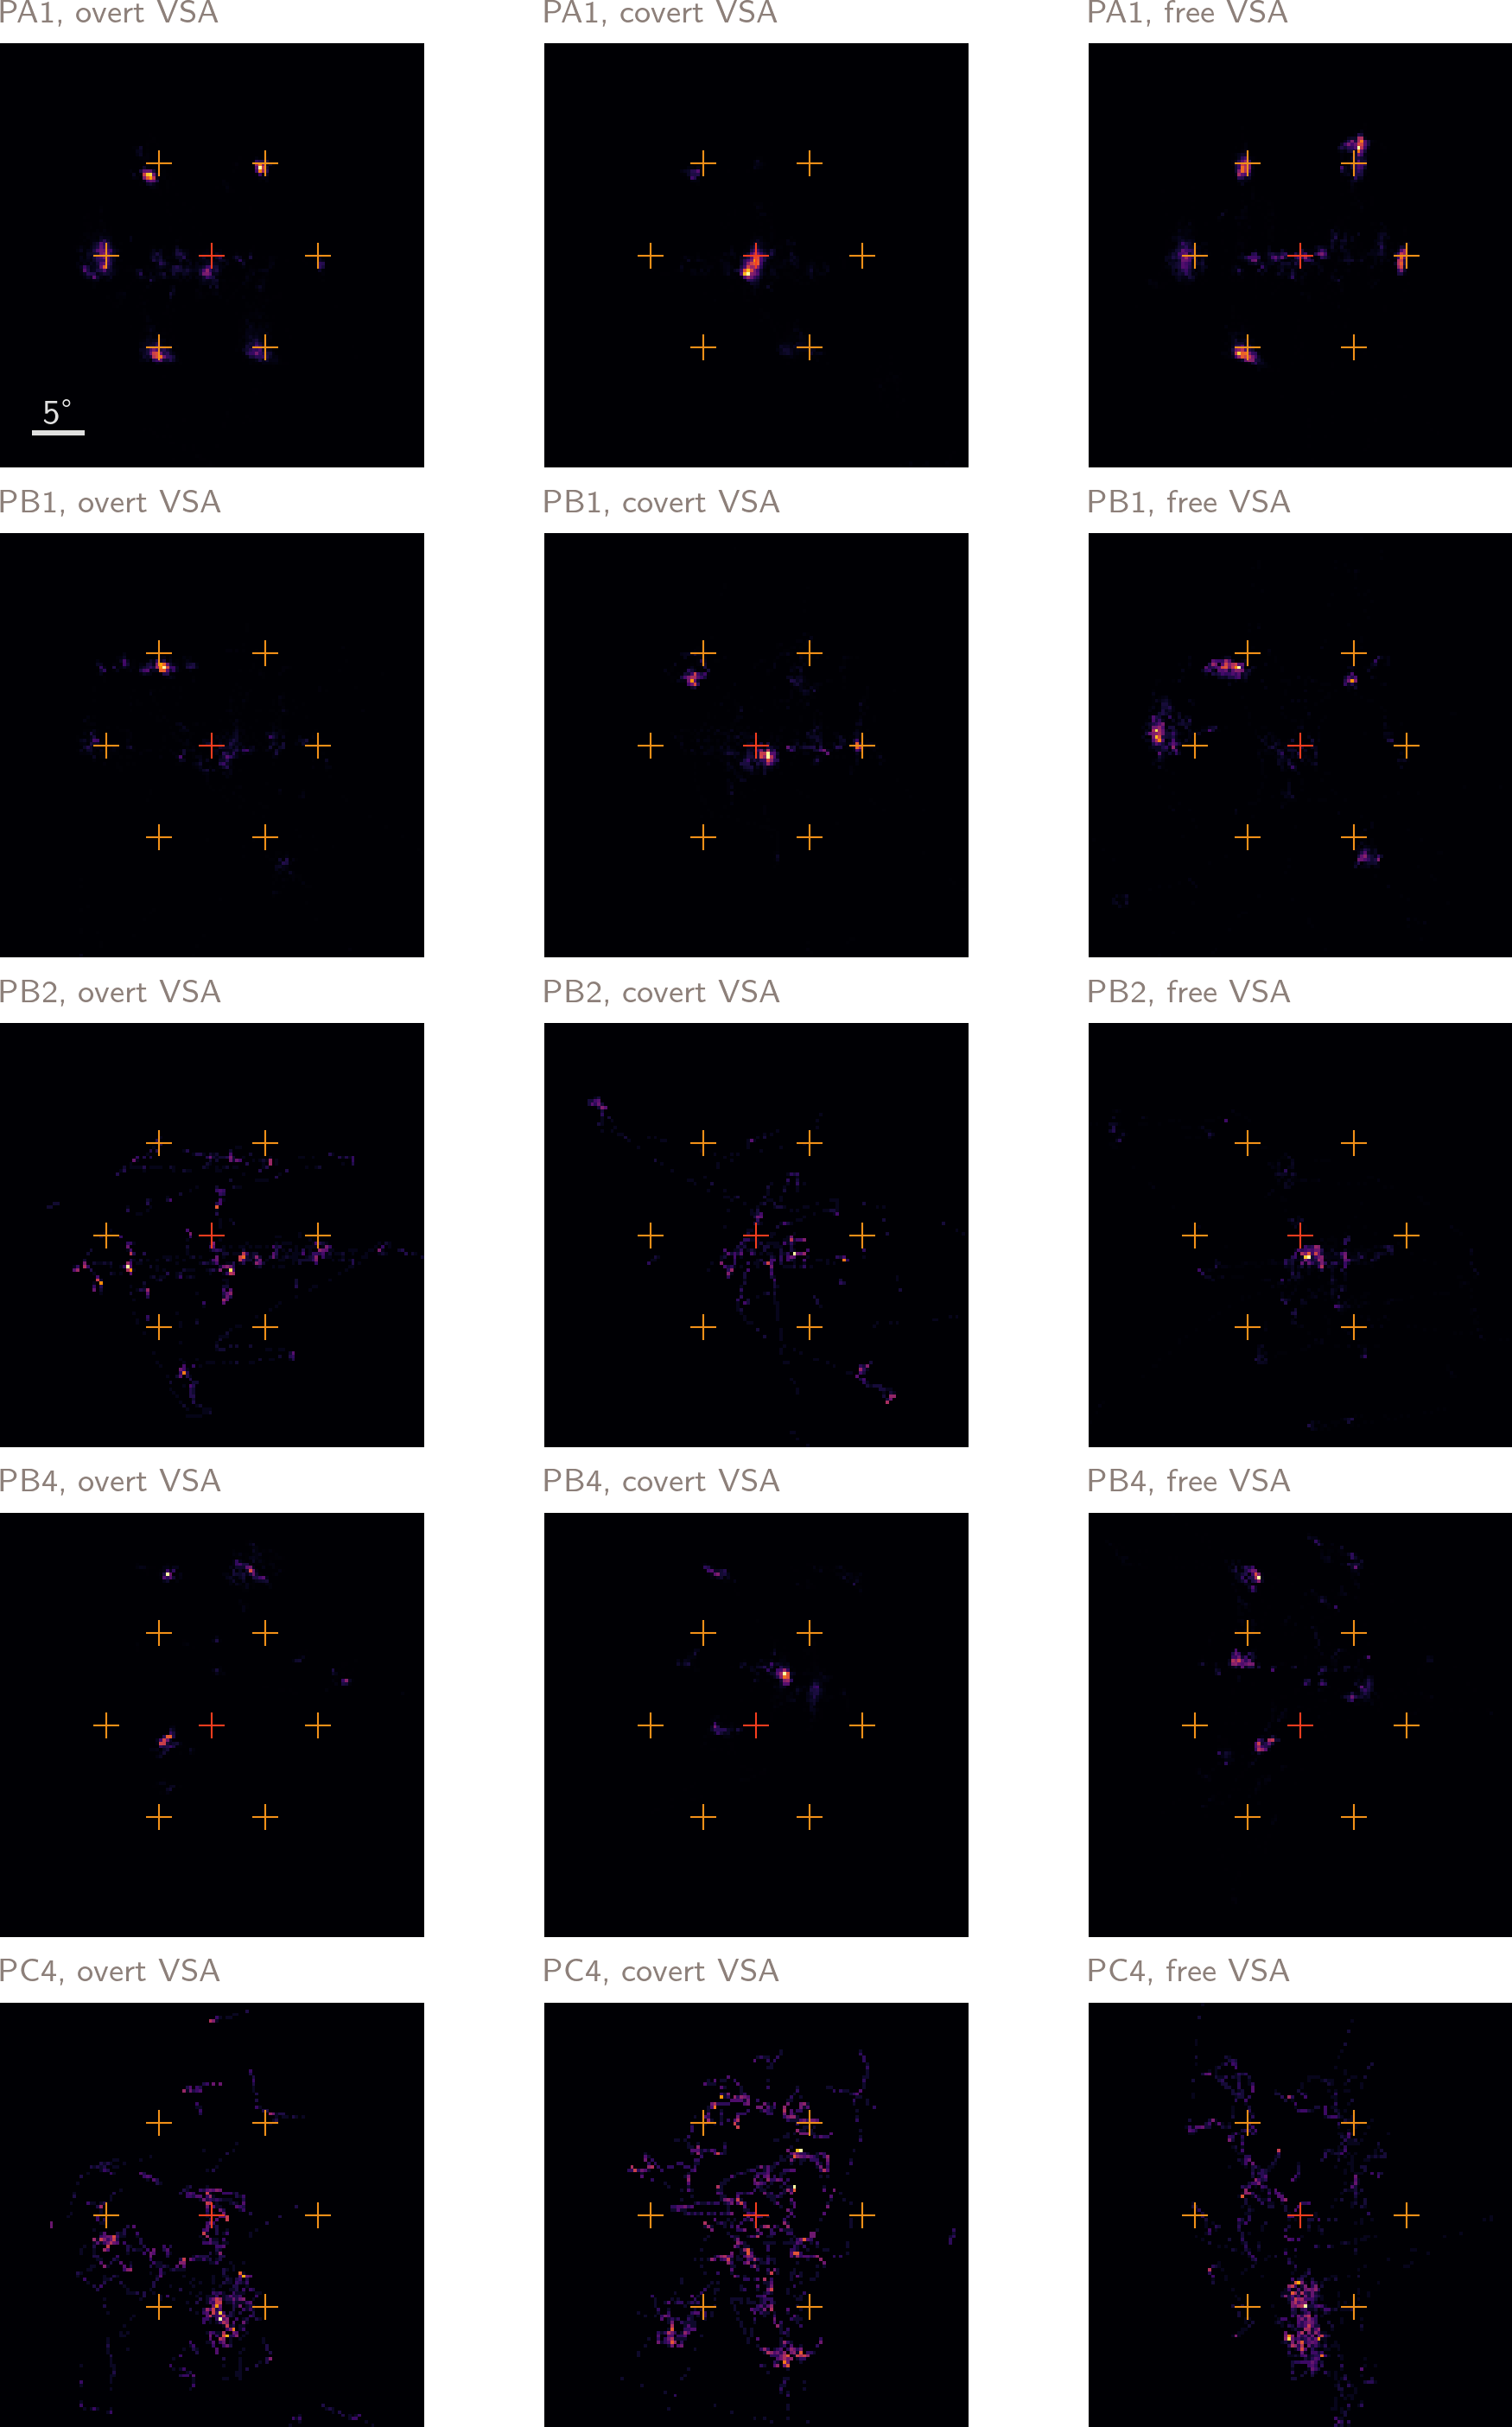
\includegraphics[width=\textwidth]{figures/patients/fig_gaze.png}
}{%
  Distribution of the recorded gaze position during the experimental session in the three \ac{vsa}
  conditions.
  Subjects PB2 and PC4 preferred covert \ac{bci} operation, with PB2 resting gaze
  near the middle of the screen, and PC4 near the bottom.
}{%
  fig:patients/gaze
}
\todo{explaine crosses}

PA1 had relatively intact gaze control and was able to correctly perform the
cued overt and covert settings.
When gaze was uncued he fixated the cued target.
This was also mostly the case for PB1, although eye tracking revealed that he
chose not to perform central gaze fixation when cued in at least one of the
stimulation blocks. We were unable to record his gaze near the bottom left
stimulus position, either due to eye tracker failure or because the participant
was not comfortable fixating this position.
Eye tracker calibration did not succeed for subject PB4, but given
transformations of gaze positions to the stimulus space, thy

PB2 was able to perform overt \ac{vsa} and central fixation to some extent,
yet eye tracking, but gaze position distributions shows a larger spread than
for PA1 and PB1.
The distribution in free \ac{vsa}, however, showed that she prefered to attend
stimuli covertly when the gaze was uncued.
This was confirmed by the participant.

The overt and central gaze fixation settings were also not properly adapted to
particpant PC4.
In free \ac{vsa} eye tracker results show that his gaze was usually near the
bottom two targets, indicating some degree of covert or split \ac{vsa}.

It was technically impossible to register gaze position with the Tobii
\todo{model} for participants PC2 and PC3 since they both had one eye that was
occluded respectively by the prism glass and the eyelid.
Both participants reported they could not fixate some of the
stimuli.

\subsection{\Ac{bci} decoding performance}

Figure~\ref{fig:patients/decode} shows single-trial
\ac{rocauc} in the evaluated \ac{vsa} settings fort the different decoders.
Scores were obtained using 6-fold cross-validation where folds corresponded to
stimulation blocks.

\begin{figure}[t]
  \hspace{-0.16816613518892673in}
%% Creator: Matplotlib, PGF backend
%%
%% To include the figure in your LaTeX document, write
%%   \input{<filename>.pgf}
%%
%% Make sure the required packages are loaded in your preamble
%%   \usepackage{pgf}
%%
%% Also ensure that all the required font packages are loaded; for instance,
%% the lmodern package is sometimes necessary when using math font.
%%   \usepackage{lmodern}
%%
%% Figures using additional raster images can only be included by \input if
%% they are in the same directory as the main LaTeX file. For loading figures
%% from other directories you can use the `import` package
%%   \usepackage{import}
%%
%% and then include the figures with
%%   \import{<path to file>}{<filename>.pgf}
%%
%% Matplotlib used the following preamble
%%
\begingroup%
\makeatletter%
\begin{pgfpicture}%
\pgfpathrectangle{\pgfpointorigin}{\pgfqpoint{4.941931in}{2.000000in}}%
\pgfusepath{use as bounding box, clip}%
\begin{pgfscope}%
\pgfsetbuttcap%
\pgfsetmiterjoin%
\definecolor{currentfill}{rgb}{1.000000,1.000000,1.000000}%
\pgfsetfillcolor{currentfill}%
\pgfsetlinewidth{0.000000pt}%
\definecolor{currentstroke}{rgb}{1.000000,1.000000,1.000000}%
\pgfsetstrokecolor{currentstroke}%
\pgfsetdash{}{0pt}%
\pgfpathmoveto{\pgfqpoint{0.000000in}{0.000000in}}%
\pgfpathlineto{\pgfqpoint{4.941931in}{0.000000in}}%
\pgfpathlineto{\pgfqpoint{4.941931in}{2.000000in}}%
\pgfpathlineto{\pgfqpoint{0.000000in}{2.000000in}}%
\pgfpathlineto{\pgfqpoint{0.000000in}{0.000000in}}%
\pgfpathclose%
\pgfusepath{fill}%
\end{pgfscope}%
\begin{pgfscope}%
\pgfsetbuttcap%
\pgfsetmiterjoin%
\definecolor{currentfill}{rgb}{1.000000,1.000000,1.000000}%
\pgfsetfillcolor{currentfill}%
\pgfsetlinewidth{0.000000pt}%
\definecolor{currentstroke}{rgb}{0.000000,0.000000,0.000000}%
\pgfsetstrokecolor{currentstroke}%
\pgfsetstrokeopacity{0.000000}%
\pgfsetdash{}{0pt}%
\pgfpathmoveto{\pgfqpoint{0.174090in}{0.190223in}}%
\pgfpathlineto{\pgfqpoint{1.713951in}{0.190223in}}%
\pgfpathlineto{\pgfqpoint{1.713951in}{1.872074in}}%
\pgfpathlineto{\pgfqpoint{0.174090in}{1.872074in}}%
\pgfpathlineto{\pgfqpoint{0.174090in}{0.190223in}}%
\pgfpathclose%
\pgfusepath{fill}%
\end{pgfscope}%
\begin{pgfscope}%
\pgfpathrectangle{\pgfqpoint{0.174090in}{0.190223in}}{\pgfqpoint{1.539861in}{1.681851in}}%
\pgfusepath{clip}%
\pgfsetbuttcap%
\pgfsetmiterjoin%
\definecolor{currentfill}{rgb}{0.842157,0.553922,0.200980}%
\pgfsetfillcolor{currentfill}%
\pgfsetlinewidth{0.000000pt}%
\definecolor{currentstroke}{rgb}{0.000000,0.000000,0.000000}%
\pgfsetstrokecolor{currentstroke}%
\pgfsetstrokeopacity{0.000000}%
\pgfsetdash{}{0pt}%
\pgfpathmoveto{\pgfqpoint{0.193338in}{0.190223in}}%
\pgfpathlineto{\pgfqpoint{0.244667in}{0.190223in}}%
\pgfpathlineto{\pgfqpoint{0.244667in}{1.317977in}}%
\pgfpathlineto{\pgfqpoint{0.193338in}{1.317977in}}%
\pgfpathlineto{\pgfqpoint{0.193338in}{0.190223in}}%
\pgfpathclose%
\pgfusepath{fill}%
\end{pgfscope}%
\begin{pgfscope}%
\pgfpathrectangle{\pgfqpoint{0.174090in}{0.190223in}}{\pgfqpoint{1.539861in}{1.681851in}}%
\pgfusepath{clip}%
\pgfsetbuttcap%
\pgfsetmiterjoin%
\definecolor{currentfill}{rgb}{0.842157,0.553922,0.200980}%
\pgfsetfillcolor{currentfill}%
\pgfsetlinewidth{0.000000pt}%
\definecolor{currentstroke}{rgb}{0.000000,0.000000,0.000000}%
\pgfsetstrokecolor{currentstroke}%
\pgfsetstrokeopacity{0.000000}%
\pgfsetdash{}{0pt}%
\pgfpathmoveto{\pgfqpoint{0.385821in}{0.190223in}}%
\pgfpathlineto{\pgfqpoint{0.437150in}{0.190223in}}%
\pgfpathlineto{\pgfqpoint{0.437150in}{1.717496in}}%
\pgfpathlineto{\pgfqpoint{0.385821in}{1.717496in}}%
\pgfpathlineto{\pgfqpoint{0.385821in}{0.190223in}}%
\pgfpathclose%
\pgfusepath{fill}%
\end{pgfscope}%
\begin{pgfscope}%
\pgfpathrectangle{\pgfqpoint{0.174090in}{0.190223in}}{\pgfqpoint{1.539861in}{1.681851in}}%
\pgfusepath{clip}%
\pgfsetbuttcap%
\pgfsetmiterjoin%
\definecolor{currentfill}{rgb}{0.842157,0.553922,0.200980}%
\pgfsetfillcolor{currentfill}%
\pgfsetlinewidth{0.000000pt}%
\definecolor{currentstroke}{rgb}{0.000000,0.000000,0.000000}%
\pgfsetstrokecolor{currentstroke}%
\pgfsetstrokeopacity{0.000000}%
\pgfsetdash{}{0pt}%
\pgfpathmoveto{\pgfqpoint{0.578304in}{0.190223in}}%
\pgfpathlineto{\pgfqpoint{0.629632in}{0.190223in}}%
\pgfpathlineto{\pgfqpoint{0.629632in}{1.589719in}}%
\pgfpathlineto{\pgfqpoint{0.578304in}{1.589719in}}%
\pgfpathlineto{\pgfqpoint{0.578304in}{0.190223in}}%
\pgfpathclose%
\pgfusepath{fill}%
\end{pgfscope}%
\begin{pgfscope}%
\pgfpathrectangle{\pgfqpoint{0.174090in}{0.190223in}}{\pgfqpoint{1.539861in}{1.681851in}}%
\pgfusepath{clip}%
\pgfsetbuttcap%
\pgfsetmiterjoin%
\definecolor{currentfill}{rgb}{0.842157,0.553922,0.200980}%
\pgfsetfillcolor{currentfill}%
\pgfsetlinewidth{0.000000pt}%
\definecolor{currentstroke}{rgb}{0.000000,0.000000,0.000000}%
\pgfsetstrokecolor{currentstroke}%
\pgfsetstrokeopacity{0.000000}%
\pgfsetdash{}{0pt}%
\pgfpathmoveto{\pgfqpoint{0.770786in}{0.190223in}}%
\pgfpathlineto{\pgfqpoint{0.822115in}{0.190223in}}%
\pgfpathlineto{\pgfqpoint{0.822115in}{1.589345in}}%
\pgfpathlineto{\pgfqpoint{0.770786in}{1.589345in}}%
\pgfpathlineto{\pgfqpoint{0.770786in}{0.190223in}}%
\pgfpathclose%
\pgfusepath{fill}%
\end{pgfscope}%
\begin{pgfscope}%
\pgfpathrectangle{\pgfqpoint{0.174090in}{0.190223in}}{\pgfqpoint{1.539861in}{1.681851in}}%
\pgfusepath{clip}%
\pgfsetbuttcap%
\pgfsetmiterjoin%
\definecolor{currentfill}{rgb}{0.842157,0.553922,0.200980}%
\pgfsetfillcolor{currentfill}%
\pgfsetlinewidth{0.000000pt}%
\definecolor{currentstroke}{rgb}{0.000000,0.000000,0.000000}%
\pgfsetstrokecolor{currentstroke}%
\pgfsetstrokeopacity{0.000000}%
\pgfsetdash{}{0pt}%
\pgfpathmoveto{\pgfqpoint{0.963269in}{0.190223in}}%
\pgfpathlineto{\pgfqpoint{1.014598in}{0.190223in}}%
\pgfpathlineto{\pgfqpoint{1.014598in}{1.384946in}}%
\pgfpathlineto{\pgfqpoint{0.963269in}{1.384946in}}%
\pgfpathlineto{\pgfqpoint{0.963269in}{0.190223in}}%
\pgfpathclose%
\pgfusepath{fill}%
\end{pgfscope}%
\begin{pgfscope}%
\pgfpathrectangle{\pgfqpoint{0.174090in}{0.190223in}}{\pgfqpoint{1.539861in}{1.681851in}}%
\pgfusepath{clip}%
\pgfsetbuttcap%
\pgfsetmiterjoin%
\definecolor{currentfill}{rgb}{0.842157,0.553922,0.200980}%
\pgfsetfillcolor{currentfill}%
\pgfsetlinewidth{0.000000pt}%
\definecolor{currentstroke}{rgb}{0.000000,0.000000,0.000000}%
\pgfsetstrokecolor{currentstroke}%
\pgfsetstrokeopacity{0.000000}%
\pgfsetdash{}{0pt}%
\pgfpathmoveto{\pgfqpoint{1.155752in}{0.190223in}}%
\pgfpathlineto{\pgfqpoint{1.207080in}{0.190223in}}%
\pgfpathlineto{\pgfqpoint{1.207080in}{1.375840in}}%
\pgfpathlineto{\pgfqpoint{1.155752in}{1.375840in}}%
\pgfpathlineto{\pgfqpoint{1.155752in}{0.190223in}}%
\pgfpathclose%
\pgfusepath{fill}%
\end{pgfscope}%
\begin{pgfscope}%
\pgfpathrectangle{\pgfqpoint{0.174090in}{0.190223in}}{\pgfqpoint{1.539861in}{1.681851in}}%
\pgfusepath{clip}%
\pgfsetbuttcap%
\pgfsetmiterjoin%
\definecolor{currentfill}{rgb}{0.842157,0.553922,0.200980}%
\pgfsetfillcolor{currentfill}%
\pgfsetlinewidth{0.000000pt}%
\definecolor{currentstroke}{rgb}{0.000000,0.000000,0.000000}%
\pgfsetstrokecolor{currentstroke}%
\pgfsetstrokeopacity{0.000000}%
\pgfsetdash{}{0pt}%
\pgfpathmoveto{\pgfqpoint{1.348234in}{0.190223in}}%
\pgfpathlineto{\pgfqpoint{1.399563in}{0.190223in}}%
\pgfpathlineto{\pgfqpoint{1.399563in}{1.302232in}}%
\pgfpathlineto{\pgfqpoint{1.348234in}{1.302232in}}%
\pgfpathlineto{\pgfqpoint{1.348234in}{0.190223in}}%
\pgfpathclose%
\pgfusepath{fill}%
\end{pgfscope}%
\begin{pgfscope}%
\pgfpathrectangle{\pgfqpoint{0.174090in}{0.190223in}}{\pgfqpoint{1.539861in}{1.681851in}}%
\pgfusepath{clip}%
\pgfsetbuttcap%
\pgfsetmiterjoin%
\definecolor{currentfill}{rgb}{0.842157,0.553922,0.200980}%
\pgfsetfillcolor{currentfill}%
\pgfsetlinewidth{0.000000pt}%
\definecolor{currentstroke}{rgb}{0.000000,0.000000,0.000000}%
\pgfsetstrokecolor{currentstroke}%
\pgfsetstrokeopacity{0.000000}%
\pgfsetdash{}{0pt}%
\pgfpathmoveto{\pgfqpoint{1.540717in}{0.190223in}}%
\pgfpathlineto{\pgfqpoint{1.592046in}{0.190223in}}%
\pgfpathlineto{\pgfqpoint{1.592046in}{1.468222in}}%
\pgfpathlineto{\pgfqpoint{1.540717in}{1.468222in}}%
\pgfpathlineto{\pgfqpoint{1.540717in}{0.190223in}}%
\pgfpathclose%
\pgfusepath{fill}%
\end{pgfscope}%
\begin{pgfscope}%
\pgfpathrectangle{\pgfqpoint{0.174090in}{0.190223in}}{\pgfqpoint{1.539861in}{1.681851in}}%
\pgfusepath{clip}%
\pgfsetbuttcap%
\pgfsetmiterjoin%
\definecolor{currentfill}{rgb}{0.858824,0.314706,0.223529}%
\pgfsetfillcolor{currentfill}%
\pgfsetlinewidth{0.000000pt}%
\definecolor{currentstroke}{rgb}{0.000000,0.000000,0.000000}%
\pgfsetstrokecolor{currentstroke}%
\pgfsetstrokeopacity{0.000000}%
\pgfsetdash{}{0pt}%
\pgfpathmoveto{\pgfqpoint{0.244667in}{0.190223in}}%
\pgfpathlineto{\pgfqpoint{0.295996in}{0.190223in}}%
\pgfpathlineto{\pgfqpoint{0.295996in}{1.393596in}}%
\pgfpathlineto{\pgfqpoint{0.244667in}{1.393596in}}%
\pgfpathlineto{\pgfqpoint{0.244667in}{0.190223in}}%
\pgfpathclose%
\pgfusepath{fill}%
\end{pgfscope}%
\begin{pgfscope}%
\pgfpathrectangle{\pgfqpoint{0.174090in}{0.190223in}}{\pgfqpoint{1.539861in}{1.681851in}}%
\pgfusepath{clip}%
\pgfsetbuttcap%
\pgfsetmiterjoin%
\definecolor{currentfill}{rgb}{0.858824,0.314706,0.223529}%
\pgfsetfillcolor{currentfill}%
\pgfsetlinewidth{0.000000pt}%
\definecolor{currentstroke}{rgb}{0.000000,0.000000,0.000000}%
\pgfsetstrokecolor{currentstroke}%
\pgfsetstrokeopacity{0.000000}%
\pgfsetdash{}{0pt}%
\pgfpathmoveto{\pgfqpoint{0.437150in}{0.190223in}}%
\pgfpathlineto{\pgfqpoint{0.488478in}{0.190223in}}%
\pgfpathlineto{\pgfqpoint{0.488478in}{1.695290in}}%
\pgfpathlineto{\pgfqpoint{0.437150in}{1.695290in}}%
\pgfpathlineto{\pgfqpoint{0.437150in}{0.190223in}}%
\pgfpathclose%
\pgfusepath{fill}%
\end{pgfscope}%
\begin{pgfscope}%
\pgfpathrectangle{\pgfqpoint{0.174090in}{0.190223in}}{\pgfqpoint{1.539861in}{1.681851in}}%
\pgfusepath{clip}%
\pgfsetbuttcap%
\pgfsetmiterjoin%
\definecolor{currentfill}{rgb}{0.858824,0.314706,0.223529}%
\pgfsetfillcolor{currentfill}%
\pgfsetlinewidth{0.000000pt}%
\definecolor{currentstroke}{rgb}{0.000000,0.000000,0.000000}%
\pgfsetstrokecolor{currentstroke}%
\pgfsetstrokeopacity{0.000000}%
\pgfsetdash{}{0pt}%
\pgfpathmoveto{\pgfqpoint{0.629632in}{0.190223in}}%
\pgfpathlineto{\pgfqpoint{0.680961in}{0.190223in}}%
\pgfpathlineto{\pgfqpoint{0.680961in}{1.582085in}}%
\pgfpathlineto{\pgfqpoint{0.629632in}{1.582085in}}%
\pgfpathlineto{\pgfqpoint{0.629632in}{0.190223in}}%
\pgfpathclose%
\pgfusepath{fill}%
\end{pgfscope}%
\begin{pgfscope}%
\pgfpathrectangle{\pgfqpoint{0.174090in}{0.190223in}}{\pgfqpoint{1.539861in}{1.681851in}}%
\pgfusepath{clip}%
\pgfsetbuttcap%
\pgfsetmiterjoin%
\definecolor{currentfill}{rgb}{0.858824,0.314706,0.223529}%
\pgfsetfillcolor{currentfill}%
\pgfsetlinewidth{0.000000pt}%
\definecolor{currentstroke}{rgb}{0.000000,0.000000,0.000000}%
\pgfsetstrokecolor{currentstroke}%
\pgfsetstrokeopacity{0.000000}%
\pgfsetdash{}{0pt}%
\pgfpathmoveto{\pgfqpoint{0.822115in}{0.190223in}}%
\pgfpathlineto{\pgfqpoint{0.873444in}{0.190223in}}%
\pgfpathlineto{\pgfqpoint{0.873444in}{1.544680in}}%
\pgfpathlineto{\pgfqpoint{0.822115in}{1.544680in}}%
\pgfpathlineto{\pgfqpoint{0.822115in}{0.190223in}}%
\pgfpathclose%
\pgfusepath{fill}%
\end{pgfscope}%
\begin{pgfscope}%
\pgfpathrectangle{\pgfqpoint{0.174090in}{0.190223in}}{\pgfqpoint{1.539861in}{1.681851in}}%
\pgfusepath{clip}%
\pgfsetbuttcap%
\pgfsetmiterjoin%
\definecolor{currentfill}{rgb}{0.858824,0.314706,0.223529}%
\pgfsetfillcolor{currentfill}%
\pgfsetlinewidth{0.000000pt}%
\definecolor{currentstroke}{rgb}{0.000000,0.000000,0.000000}%
\pgfsetstrokecolor{currentstroke}%
\pgfsetstrokeopacity{0.000000}%
\pgfsetdash{}{0pt}%
\pgfpathmoveto{\pgfqpoint{1.014598in}{0.190223in}}%
\pgfpathlineto{\pgfqpoint{1.065926in}{0.190223in}}%
\pgfpathlineto{\pgfqpoint{1.065926in}{1.346833in}}%
\pgfpathlineto{\pgfqpoint{1.014598in}{1.346833in}}%
\pgfpathlineto{\pgfqpoint{1.014598in}{0.190223in}}%
\pgfpathclose%
\pgfusepath{fill}%
\end{pgfscope}%
\begin{pgfscope}%
\pgfpathrectangle{\pgfqpoint{0.174090in}{0.190223in}}{\pgfqpoint{1.539861in}{1.681851in}}%
\pgfusepath{clip}%
\pgfsetbuttcap%
\pgfsetmiterjoin%
\definecolor{currentfill}{rgb}{0.858824,0.314706,0.223529}%
\pgfsetfillcolor{currentfill}%
\pgfsetlinewidth{0.000000pt}%
\definecolor{currentstroke}{rgb}{0.000000,0.000000,0.000000}%
\pgfsetstrokecolor{currentstroke}%
\pgfsetstrokeopacity{0.000000}%
\pgfsetdash{}{0pt}%
\pgfpathmoveto{\pgfqpoint{1.207080in}{0.190223in}}%
\pgfpathlineto{\pgfqpoint{1.258409in}{0.190223in}}%
\pgfpathlineto{\pgfqpoint{1.258409in}{1.372747in}}%
\pgfpathlineto{\pgfqpoint{1.207080in}{1.372747in}}%
\pgfpathlineto{\pgfqpoint{1.207080in}{0.190223in}}%
\pgfpathclose%
\pgfusepath{fill}%
\end{pgfscope}%
\begin{pgfscope}%
\pgfpathrectangle{\pgfqpoint{0.174090in}{0.190223in}}{\pgfqpoint{1.539861in}{1.681851in}}%
\pgfusepath{clip}%
\pgfsetbuttcap%
\pgfsetmiterjoin%
\definecolor{currentfill}{rgb}{0.858824,0.314706,0.223529}%
\pgfsetfillcolor{currentfill}%
\pgfsetlinewidth{0.000000pt}%
\definecolor{currentstroke}{rgb}{0.000000,0.000000,0.000000}%
\pgfsetstrokecolor{currentstroke}%
\pgfsetstrokeopacity{0.000000}%
\pgfsetdash{}{0pt}%
\pgfpathmoveto{\pgfqpoint{1.399563in}{0.190223in}}%
\pgfpathlineto{\pgfqpoint{1.450892in}{0.190223in}}%
\pgfpathlineto{\pgfqpoint{1.450892in}{1.294360in}}%
\pgfpathlineto{\pgfqpoint{1.399563in}{1.294360in}}%
\pgfpathlineto{\pgfqpoint{1.399563in}{0.190223in}}%
\pgfpathclose%
\pgfusepath{fill}%
\end{pgfscope}%
\begin{pgfscope}%
\pgfpathrectangle{\pgfqpoint{0.174090in}{0.190223in}}{\pgfqpoint{1.539861in}{1.681851in}}%
\pgfusepath{clip}%
\pgfsetbuttcap%
\pgfsetmiterjoin%
\definecolor{currentfill}{rgb}{0.858824,0.314706,0.223529}%
\pgfsetfillcolor{currentfill}%
\pgfsetlinewidth{0.000000pt}%
\definecolor{currentstroke}{rgb}{0.000000,0.000000,0.000000}%
\pgfsetstrokecolor{currentstroke}%
\pgfsetstrokeopacity{0.000000}%
\pgfsetdash{}{0pt}%
\pgfpathmoveto{\pgfqpoint{1.592046in}{0.190223in}}%
\pgfpathlineto{\pgfqpoint{1.643374in}{0.190223in}}%
\pgfpathlineto{\pgfqpoint{1.643374in}{1.461370in}}%
\pgfpathlineto{\pgfqpoint{1.592046in}{1.461370in}}%
\pgfpathlineto{\pgfqpoint{1.592046in}{0.190223in}}%
\pgfpathclose%
\pgfusepath{fill}%
\end{pgfscope}%
\begin{pgfscope}%
\pgfpathrectangle{\pgfqpoint{0.174090in}{0.190223in}}{\pgfqpoint{1.539861in}{1.681851in}}%
\pgfusepath{clip}%
\pgfsetbuttcap%
\pgfsetmiterjoin%
\definecolor{currentfill}{rgb}{0.464706,0.320588,0.573529}%
\pgfsetfillcolor{currentfill}%
\pgfsetlinewidth{0.000000pt}%
\definecolor{currentstroke}{rgb}{0.000000,0.000000,0.000000}%
\pgfsetstrokecolor{currentstroke}%
\pgfsetstrokeopacity{0.000000}%
\pgfsetdash{}{0pt}%
\pgfpathmoveto{\pgfqpoint{0.295996in}{0.190223in}}%
\pgfpathlineto{\pgfqpoint{0.347325in}{0.190223in}}%
\pgfpathlineto{\pgfqpoint{0.347325in}{1.332130in}}%
\pgfpathlineto{\pgfqpoint{0.295996in}{1.332130in}}%
\pgfpathlineto{\pgfqpoint{0.295996in}{0.190223in}}%
\pgfpathclose%
\pgfusepath{fill}%
\end{pgfscope}%
\begin{pgfscope}%
\pgfpathrectangle{\pgfqpoint{0.174090in}{0.190223in}}{\pgfqpoint{1.539861in}{1.681851in}}%
\pgfusepath{clip}%
\pgfsetbuttcap%
\pgfsetmiterjoin%
\definecolor{currentfill}{rgb}{0.464706,0.320588,0.573529}%
\pgfsetfillcolor{currentfill}%
\pgfsetlinewidth{0.000000pt}%
\definecolor{currentstroke}{rgb}{0.000000,0.000000,0.000000}%
\pgfsetstrokecolor{currentstroke}%
\pgfsetstrokeopacity{0.000000}%
\pgfsetdash{}{0pt}%
\pgfpathmoveto{\pgfqpoint{0.488478in}{0.190223in}}%
\pgfpathlineto{\pgfqpoint{0.539807in}{0.190223in}}%
\pgfpathlineto{\pgfqpoint{0.539807in}{1.696667in}}%
\pgfpathlineto{\pgfqpoint{0.488478in}{1.696667in}}%
\pgfpathlineto{\pgfqpoint{0.488478in}{0.190223in}}%
\pgfpathclose%
\pgfusepath{fill}%
\end{pgfscope}%
\begin{pgfscope}%
\pgfpathrectangle{\pgfqpoint{0.174090in}{0.190223in}}{\pgfqpoint{1.539861in}{1.681851in}}%
\pgfusepath{clip}%
\pgfsetbuttcap%
\pgfsetmiterjoin%
\definecolor{currentfill}{rgb}{0.464706,0.320588,0.573529}%
\pgfsetfillcolor{currentfill}%
\pgfsetlinewidth{0.000000pt}%
\definecolor{currentstroke}{rgb}{0.000000,0.000000,0.000000}%
\pgfsetstrokecolor{currentstroke}%
\pgfsetstrokeopacity{0.000000}%
\pgfsetdash{}{0pt}%
\pgfpathmoveto{\pgfqpoint{0.680961in}{0.190223in}}%
\pgfpathlineto{\pgfqpoint{0.732290in}{0.190223in}}%
\pgfpathlineto{\pgfqpoint{0.732290in}{1.548223in}}%
\pgfpathlineto{\pgfqpoint{0.680961in}{1.548223in}}%
\pgfpathlineto{\pgfqpoint{0.680961in}{0.190223in}}%
\pgfpathclose%
\pgfusepath{fill}%
\end{pgfscope}%
\begin{pgfscope}%
\pgfpathrectangle{\pgfqpoint{0.174090in}{0.190223in}}{\pgfqpoint{1.539861in}{1.681851in}}%
\pgfusepath{clip}%
\pgfsetbuttcap%
\pgfsetmiterjoin%
\definecolor{currentfill}{rgb}{0.464706,0.320588,0.573529}%
\pgfsetfillcolor{currentfill}%
\pgfsetlinewidth{0.000000pt}%
\definecolor{currentstroke}{rgb}{0.000000,0.000000,0.000000}%
\pgfsetstrokecolor{currentstroke}%
\pgfsetstrokeopacity{0.000000}%
\pgfsetdash{}{0pt}%
\pgfpathmoveto{\pgfqpoint{0.873444in}{0.190223in}}%
\pgfpathlineto{\pgfqpoint{0.924772in}{0.190223in}}%
\pgfpathlineto{\pgfqpoint{0.924772in}{1.582413in}}%
\pgfpathlineto{\pgfqpoint{0.873444in}{1.582413in}}%
\pgfpathlineto{\pgfqpoint{0.873444in}{0.190223in}}%
\pgfpathclose%
\pgfusepath{fill}%
\end{pgfscope}%
\begin{pgfscope}%
\pgfpathrectangle{\pgfqpoint{0.174090in}{0.190223in}}{\pgfqpoint{1.539861in}{1.681851in}}%
\pgfusepath{clip}%
\pgfsetbuttcap%
\pgfsetmiterjoin%
\definecolor{currentfill}{rgb}{0.464706,0.320588,0.573529}%
\pgfsetfillcolor{currentfill}%
\pgfsetlinewidth{0.000000pt}%
\definecolor{currentstroke}{rgb}{0.000000,0.000000,0.000000}%
\pgfsetstrokecolor{currentstroke}%
\pgfsetstrokeopacity{0.000000}%
\pgfsetdash{}{0pt}%
\pgfpathmoveto{\pgfqpoint{1.065926in}{0.190223in}}%
\pgfpathlineto{\pgfqpoint{1.117255in}{0.190223in}}%
\pgfpathlineto{\pgfqpoint{1.117255in}{1.389045in}}%
\pgfpathlineto{\pgfqpoint{1.065926in}{1.389045in}}%
\pgfpathlineto{\pgfqpoint{1.065926in}{0.190223in}}%
\pgfpathclose%
\pgfusepath{fill}%
\end{pgfscope}%
\begin{pgfscope}%
\pgfpathrectangle{\pgfqpoint{0.174090in}{0.190223in}}{\pgfqpoint{1.539861in}{1.681851in}}%
\pgfusepath{clip}%
\pgfsetbuttcap%
\pgfsetmiterjoin%
\definecolor{currentfill}{rgb}{0.464706,0.320588,0.573529}%
\pgfsetfillcolor{currentfill}%
\pgfsetlinewidth{0.000000pt}%
\definecolor{currentstroke}{rgb}{0.000000,0.000000,0.000000}%
\pgfsetstrokecolor{currentstroke}%
\pgfsetstrokeopacity{0.000000}%
\pgfsetdash{}{0pt}%
\pgfpathmoveto{\pgfqpoint{1.258409in}{0.190223in}}%
\pgfpathlineto{\pgfqpoint{1.309738in}{0.190223in}}%
\pgfpathlineto{\pgfqpoint{1.309738in}{1.289552in}}%
\pgfpathlineto{\pgfqpoint{1.258409in}{1.289552in}}%
\pgfpathlineto{\pgfqpoint{1.258409in}{0.190223in}}%
\pgfpathclose%
\pgfusepath{fill}%
\end{pgfscope}%
\begin{pgfscope}%
\pgfpathrectangle{\pgfqpoint{0.174090in}{0.190223in}}{\pgfqpoint{1.539861in}{1.681851in}}%
\pgfusepath{clip}%
\pgfsetbuttcap%
\pgfsetmiterjoin%
\definecolor{currentfill}{rgb}{0.464706,0.320588,0.573529}%
\pgfsetfillcolor{currentfill}%
\pgfsetlinewidth{0.000000pt}%
\definecolor{currentstroke}{rgb}{0.000000,0.000000,0.000000}%
\pgfsetstrokecolor{currentstroke}%
\pgfsetstrokeopacity{0.000000}%
\pgfsetdash{}{0pt}%
\pgfpathmoveto{\pgfqpoint{1.450892in}{0.190223in}}%
\pgfpathlineto{\pgfqpoint{1.502220in}{0.190223in}}%
\pgfpathlineto{\pgfqpoint{1.502220in}{1.233230in}}%
\pgfpathlineto{\pgfqpoint{1.450892in}{1.233230in}}%
\pgfpathlineto{\pgfqpoint{1.450892in}{0.190223in}}%
\pgfpathclose%
\pgfusepath{fill}%
\end{pgfscope}%
\begin{pgfscope}%
\pgfpathrectangle{\pgfqpoint{0.174090in}{0.190223in}}{\pgfqpoint{1.539861in}{1.681851in}}%
\pgfusepath{clip}%
\pgfsetbuttcap%
\pgfsetmiterjoin%
\definecolor{currentfill}{rgb}{0.464706,0.320588,0.573529}%
\pgfsetfillcolor{currentfill}%
\pgfsetlinewidth{0.000000pt}%
\definecolor{currentstroke}{rgb}{0.000000,0.000000,0.000000}%
\pgfsetstrokecolor{currentstroke}%
\pgfsetstrokeopacity{0.000000}%
\pgfsetdash{}{0pt}%
\pgfpathmoveto{\pgfqpoint{1.643374in}{0.190223in}}%
\pgfpathlineto{\pgfqpoint{1.694703in}{0.190223in}}%
\pgfpathlineto{\pgfqpoint{1.694703in}{1.438751in}}%
\pgfpathlineto{\pgfqpoint{1.643374in}{1.438751in}}%
\pgfpathlineto{\pgfqpoint{1.643374in}{0.190223in}}%
\pgfpathclose%
\pgfusepath{fill}%
\end{pgfscope}%
\begin{pgfscope}%
\pgfsetbuttcap%
\pgfsetroundjoin%
\definecolor{currentfill}{rgb}{0.552941,0.501961,0.478431}%
\pgfsetfillcolor{currentfill}%
\pgfsetlinewidth{0.803000pt}%
\definecolor{currentstroke}{rgb}{0.552941,0.501961,0.478431}%
\pgfsetstrokecolor{currentstroke}%
\pgfsetdash{}{0pt}%
\pgfsys@defobject{currentmarker}{\pgfqpoint{0.000000in}{0.000000in}}{\pgfqpoint{0.000000in}{0.041667in}}{%
\pgfpathmoveto{\pgfqpoint{0.000000in}{0.000000in}}%
\pgfpathlineto{\pgfqpoint{0.000000in}{0.041667in}}%
\pgfusepath{stroke,fill}%
}%
\begin{pgfscope}%
\pgfsys@transformshift{0.270331in}{0.190223in}%
\pgfsys@useobject{currentmarker}{}%
\end{pgfscope}%
\end{pgfscope}%
\begin{pgfscope}%
\definecolor{textcolor}{rgb}{0.552941,0.501961,0.478431}%
\pgfsetstrokecolor{textcolor}%
\pgfsetfillcolor{textcolor}%
\pgftext[x=0.301581in, y=-0.079933in, left, base,rotate=90.000000]{\color{textcolor}\sffamily\fontsize{9.000000}{10.800000}\selectfont PA1}%
\end{pgfscope}%
\begin{pgfscope}%
\pgfsetbuttcap%
\pgfsetroundjoin%
\definecolor{currentfill}{rgb}{0.552941,0.501961,0.478431}%
\pgfsetfillcolor{currentfill}%
\pgfsetlinewidth{0.803000pt}%
\definecolor{currentstroke}{rgb}{0.552941,0.501961,0.478431}%
\pgfsetstrokecolor{currentstroke}%
\pgfsetdash{}{0pt}%
\pgfsys@defobject{currentmarker}{\pgfqpoint{0.000000in}{0.000000in}}{\pgfqpoint{0.000000in}{0.041667in}}{%
\pgfpathmoveto{\pgfqpoint{0.000000in}{0.000000in}}%
\pgfpathlineto{\pgfqpoint{0.000000in}{0.041667in}}%
\pgfusepath{stroke,fill}%
}%
\begin{pgfscope}%
\pgfsys@transformshift{0.462814in}{0.190223in}%
\pgfsys@useobject{currentmarker}{}%
\end{pgfscope}%
\end{pgfscope}%
\begin{pgfscope}%
\definecolor{textcolor}{rgb}{0.552941,0.501961,0.478431}%
\pgfsetstrokecolor{textcolor}%
\pgfsetfillcolor{textcolor}%
\pgftext[x=0.494064in, y=-0.090543in, left, base,rotate=90.000000]{\color{textcolor}\sffamily\fontsize{9.000000}{10.800000}\selectfont PB1}%
\end{pgfscope}%
\begin{pgfscope}%
\pgfsetbuttcap%
\pgfsetroundjoin%
\definecolor{currentfill}{rgb}{0.552941,0.501961,0.478431}%
\pgfsetfillcolor{currentfill}%
\pgfsetlinewidth{0.803000pt}%
\definecolor{currentstroke}{rgb}{0.552941,0.501961,0.478431}%
\pgfsetstrokecolor{currentstroke}%
\pgfsetdash{}{0pt}%
\pgfsys@defobject{currentmarker}{\pgfqpoint{0.000000in}{0.000000in}}{\pgfqpoint{0.000000in}{0.041667in}}{%
\pgfpathmoveto{\pgfqpoint{0.000000in}{0.000000in}}%
\pgfpathlineto{\pgfqpoint{0.000000in}{0.041667in}}%
\pgfusepath{stroke,fill}%
}%
\begin{pgfscope}%
\pgfsys@transformshift{0.655297in}{0.190223in}%
\pgfsys@useobject{currentmarker}{}%
\end{pgfscope}%
\end{pgfscope}%
\begin{pgfscope}%
\definecolor{textcolor}{rgb}{0.552941,0.501961,0.478431}%
\pgfsetstrokecolor{textcolor}%
\pgfsetfillcolor{textcolor}%
\pgftext[x=0.686547in, y=-0.090543in, left, base,rotate=90.000000]{\color{textcolor}\sffamily\fontsize{9.000000}{10.800000}\selectfont PB2}%
\end{pgfscope}%
\begin{pgfscope}%
\pgfsetbuttcap%
\pgfsetroundjoin%
\definecolor{currentfill}{rgb}{0.552941,0.501961,0.478431}%
\pgfsetfillcolor{currentfill}%
\pgfsetlinewidth{0.803000pt}%
\definecolor{currentstroke}{rgb}{0.552941,0.501961,0.478431}%
\pgfsetstrokecolor{currentstroke}%
\pgfsetdash{}{0pt}%
\pgfsys@defobject{currentmarker}{\pgfqpoint{0.000000in}{0.000000in}}{\pgfqpoint{0.000000in}{0.041667in}}{%
\pgfpathmoveto{\pgfqpoint{0.000000in}{0.000000in}}%
\pgfpathlineto{\pgfqpoint{0.000000in}{0.041667in}}%
\pgfusepath{stroke,fill}%
}%
\begin{pgfscope}%
\pgfsys@transformshift{0.847779in}{0.190223in}%
\pgfsys@useobject{currentmarker}{}%
\end{pgfscope}%
\end{pgfscope}%
\begin{pgfscope}%
\definecolor{textcolor}{rgb}{0.552941,0.501961,0.478431}%
\pgfsetstrokecolor{textcolor}%
\pgfsetfillcolor{textcolor}%
\pgftext[x=0.879029in, y=-0.090543in, left, base,rotate=90.000000]{\color{textcolor}\sffamily\fontsize{9.000000}{10.800000}\selectfont PB4}%
\end{pgfscope}%
\begin{pgfscope}%
\pgfsetbuttcap%
\pgfsetroundjoin%
\definecolor{currentfill}{rgb}{0.552941,0.501961,0.478431}%
\pgfsetfillcolor{currentfill}%
\pgfsetlinewidth{0.803000pt}%
\definecolor{currentstroke}{rgb}{0.552941,0.501961,0.478431}%
\pgfsetstrokecolor{currentstroke}%
\pgfsetdash{}{0pt}%
\pgfsys@defobject{currentmarker}{\pgfqpoint{0.000000in}{0.000000in}}{\pgfqpoint{0.000000in}{0.041667in}}{%
\pgfpathmoveto{\pgfqpoint{0.000000in}{0.000000in}}%
\pgfpathlineto{\pgfqpoint{0.000000in}{0.041667in}}%
\pgfusepath{stroke,fill}%
}%
\begin{pgfscope}%
\pgfsys@transformshift{1.040262in}{0.190223in}%
\pgfsys@useobject{currentmarker}{}%
\end{pgfscope}%
\end{pgfscope}%
\begin{pgfscope}%
\definecolor{textcolor}{rgb}{0.552941,0.501961,0.478431}%
\pgfsetstrokecolor{textcolor}%
\pgfsetfillcolor{textcolor}%
\pgftext[x=1.071512in, y=-0.086878in, left, base,rotate=90.000000]{\color{textcolor}\sffamily\fontsize{9.000000}{10.800000}\selectfont PC2}%
\end{pgfscope}%
\begin{pgfscope}%
\pgfsetbuttcap%
\pgfsetroundjoin%
\definecolor{currentfill}{rgb}{0.552941,0.501961,0.478431}%
\pgfsetfillcolor{currentfill}%
\pgfsetlinewidth{0.803000pt}%
\definecolor{currentstroke}{rgb}{0.552941,0.501961,0.478431}%
\pgfsetstrokecolor{currentstroke}%
\pgfsetdash{}{0pt}%
\pgfsys@defobject{currentmarker}{\pgfqpoint{0.000000in}{0.000000in}}{\pgfqpoint{0.000000in}{0.041667in}}{%
\pgfpathmoveto{\pgfqpoint{0.000000in}{0.000000in}}%
\pgfpathlineto{\pgfqpoint{0.000000in}{0.041667in}}%
\pgfusepath{stroke,fill}%
}%
\begin{pgfscope}%
\pgfsys@transformshift{1.232745in}{0.190223in}%
\pgfsys@useobject{currentmarker}{}%
\end{pgfscope}%
\end{pgfscope}%
\begin{pgfscope}%
\definecolor{textcolor}{rgb}{0.552941,0.501961,0.478431}%
\pgfsetstrokecolor{textcolor}%
\pgfsetfillcolor{textcolor}%
\pgftext[x=1.263995in, y=-0.086878in, left, base,rotate=90.000000]{\color{textcolor}\sffamily\fontsize{9.000000}{10.800000}\selectfont PC3}%
\end{pgfscope}%
\begin{pgfscope}%
\pgfsetbuttcap%
\pgfsetroundjoin%
\definecolor{currentfill}{rgb}{0.552941,0.501961,0.478431}%
\pgfsetfillcolor{currentfill}%
\pgfsetlinewidth{0.803000pt}%
\definecolor{currentstroke}{rgb}{0.552941,0.501961,0.478431}%
\pgfsetstrokecolor{currentstroke}%
\pgfsetdash{}{0pt}%
\pgfsys@defobject{currentmarker}{\pgfqpoint{0.000000in}{0.000000in}}{\pgfqpoint{0.000000in}{0.041667in}}{%
\pgfpathmoveto{\pgfqpoint{0.000000in}{0.000000in}}%
\pgfpathlineto{\pgfqpoint{0.000000in}{0.041667in}}%
\pgfusepath{stroke,fill}%
}%
\begin{pgfscope}%
\pgfsys@transformshift{1.425227in}{0.190223in}%
\pgfsys@useobject{currentmarker}{}%
\end{pgfscope}%
\end{pgfscope}%
\begin{pgfscope}%
\definecolor{textcolor}{rgb}{0.552941,0.501961,0.478431}%
\pgfsetstrokecolor{textcolor}%
\pgfsetfillcolor{textcolor}%
\pgftext[x=1.456477in, y=-0.086878in, left, base,rotate=90.000000]{\color{textcolor}\sffamily\fontsize{9.000000}{10.800000}\selectfont PC4}%
\end{pgfscope}%
\begin{pgfscope}%
\pgfsetbuttcap%
\pgfsetroundjoin%
\definecolor{currentfill}{rgb}{0.552941,0.501961,0.478431}%
\pgfsetfillcolor{currentfill}%
\pgfsetlinewidth{0.803000pt}%
\definecolor{currentstroke}{rgb}{0.552941,0.501961,0.478431}%
\pgfsetstrokecolor{currentstroke}%
\pgfsetdash{}{0pt}%
\pgfsys@defobject{currentmarker}{\pgfqpoint{0.000000in}{0.000000in}}{\pgfqpoint{0.000000in}{0.041667in}}{%
\pgfpathmoveto{\pgfqpoint{0.000000in}{0.000000in}}%
\pgfpathlineto{\pgfqpoint{0.000000in}{0.041667in}}%
\pgfusepath{stroke,fill}%
}%
\begin{pgfscope}%
\pgfsys@transformshift{1.617710in}{0.190223in}%
\pgfsys@useobject{currentmarker}{}%
\end{pgfscope}%
\end{pgfscope}%
\begin{pgfscope}%
\definecolor{textcolor}{rgb}{0.552941,0.501961,0.478431}%
\pgfsetstrokecolor{textcolor}%
\pgfsetfillcolor{textcolor}%
\pgftext[x=1.648960in, y=-0.079258in, left, base,rotate=90.000000]{\color{textcolor}\sffamily\fontsize{9.000000}{10.800000}\selectfont avg.}%
\end{pgfscope}%
\begin{pgfscope}%
\definecolor{textcolor}{rgb}{0.552941,0.501961,0.478431}%
\pgfsetstrokecolor{textcolor}%
\pgfsetfillcolor{textcolor}%
\pgftext[x=0.944021in,y=-0.146098in,,top]{\color{textcolor}\sffamily\fontsize{9.000000}{10.800000}\selectfont patient}%
\end{pgfscope}%
\begin{pgfscope}%
\pgfsetbuttcap%
\pgfsetroundjoin%
\definecolor{currentfill}{rgb}{0.552941,0.501961,0.478431}%
\pgfsetfillcolor{currentfill}%
\pgfsetlinewidth{0.803000pt}%
\definecolor{currentstroke}{rgb}{0.552941,0.501961,0.478431}%
\pgfsetstrokecolor{currentstroke}%
\pgfsetdash{}{0pt}%
\pgfsys@defobject{currentmarker}{\pgfqpoint{0.000000in}{0.000000in}}{\pgfqpoint{0.041667in}{0.000000in}}{%
\pgfpathmoveto{\pgfqpoint{0.000000in}{0.000000in}}%
\pgfpathlineto{\pgfqpoint{0.041667in}{0.000000in}}%
\pgfusepath{stroke,fill}%
}%
\begin{pgfscope}%
\pgfsys@transformshift{0.174090in}{0.190223in}%
\pgfsys@useobject{currentmarker}{}%
\end{pgfscope}%
\end{pgfscope}%
\begin{pgfscope}%
\definecolor{textcolor}{rgb}{0.552941,0.501961,0.478431}%
\pgfsetstrokecolor{textcolor}%
\pgfsetfillcolor{textcolor}%
\pgftext[x=-0.038679in, y=0.146821in, left, base]{\color{textcolor}\sffamily\fontsize{9.000000}{10.800000}\selectfont \(\displaystyle {0.0}\)}%
\end{pgfscope}%
\begin{pgfscope}%
\pgfsetbuttcap%
\pgfsetroundjoin%
\definecolor{currentfill}{rgb}{0.552941,0.501961,0.478431}%
\pgfsetfillcolor{currentfill}%
\pgfsetlinewidth{0.803000pt}%
\definecolor{currentstroke}{rgb}{0.552941,0.501961,0.478431}%
\pgfsetstrokecolor{currentstroke}%
\pgfsetdash{}{0pt}%
\pgfsys@defobject{currentmarker}{\pgfqpoint{0.000000in}{0.000000in}}{\pgfqpoint{0.041667in}{0.000000in}}{%
\pgfpathmoveto{\pgfqpoint{0.000000in}{0.000000in}}%
\pgfpathlineto{\pgfqpoint{0.041667in}{0.000000in}}%
\pgfusepath{stroke,fill}%
}%
\begin{pgfscope}%
\pgfsys@transformshift{0.174090in}{0.526594in}%
\pgfsys@useobject{currentmarker}{}%
\end{pgfscope}%
\end{pgfscope}%
\begin{pgfscope}%
\definecolor{textcolor}{rgb}{0.552941,0.501961,0.478431}%
\pgfsetstrokecolor{textcolor}%
\pgfsetfillcolor{textcolor}%
\pgftext[x=-0.038679in, y=0.483191in, left, base]{\color{textcolor}\sffamily\fontsize{9.000000}{10.800000}\selectfont \(\displaystyle {0.2}\)}%
\end{pgfscope}%
\begin{pgfscope}%
\pgfsetbuttcap%
\pgfsetroundjoin%
\definecolor{currentfill}{rgb}{0.552941,0.501961,0.478431}%
\pgfsetfillcolor{currentfill}%
\pgfsetlinewidth{0.803000pt}%
\definecolor{currentstroke}{rgb}{0.552941,0.501961,0.478431}%
\pgfsetstrokecolor{currentstroke}%
\pgfsetdash{}{0pt}%
\pgfsys@defobject{currentmarker}{\pgfqpoint{0.000000in}{0.000000in}}{\pgfqpoint{0.041667in}{0.000000in}}{%
\pgfpathmoveto{\pgfqpoint{0.000000in}{0.000000in}}%
\pgfpathlineto{\pgfqpoint{0.041667in}{0.000000in}}%
\pgfusepath{stroke,fill}%
}%
\begin{pgfscope}%
\pgfsys@transformshift{0.174090in}{0.862964in}%
\pgfsys@useobject{currentmarker}{}%
\end{pgfscope}%
\end{pgfscope}%
\begin{pgfscope}%
\definecolor{textcolor}{rgb}{0.552941,0.501961,0.478431}%
\pgfsetstrokecolor{textcolor}%
\pgfsetfillcolor{textcolor}%
\pgftext[x=-0.038679in, y=0.819561in, left, base]{\color{textcolor}\sffamily\fontsize{9.000000}{10.800000}\selectfont \(\displaystyle {0.4}\)}%
\end{pgfscope}%
\begin{pgfscope}%
\pgfsetbuttcap%
\pgfsetroundjoin%
\definecolor{currentfill}{rgb}{0.552941,0.501961,0.478431}%
\pgfsetfillcolor{currentfill}%
\pgfsetlinewidth{0.803000pt}%
\definecolor{currentstroke}{rgb}{0.552941,0.501961,0.478431}%
\pgfsetstrokecolor{currentstroke}%
\pgfsetdash{}{0pt}%
\pgfsys@defobject{currentmarker}{\pgfqpoint{0.000000in}{0.000000in}}{\pgfqpoint{0.041667in}{0.000000in}}{%
\pgfpathmoveto{\pgfqpoint{0.000000in}{0.000000in}}%
\pgfpathlineto{\pgfqpoint{0.041667in}{0.000000in}}%
\pgfusepath{stroke,fill}%
}%
\begin{pgfscope}%
\pgfsys@transformshift{0.174090in}{1.199334in}%
\pgfsys@useobject{currentmarker}{}%
\end{pgfscope}%
\end{pgfscope}%
\begin{pgfscope}%
\definecolor{textcolor}{rgb}{0.552941,0.501961,0.478431}%
\pgfsetstrokecolor{textcolor}%
\pgfsetfillcolor{textcolor}%
\pgftext[x=-0.038679in, y=1.155931in, left, base]{\color{textcolor}\sffamily\fontsize{9.000000}{10.800000}\selectfont \(\displaystyle {0.6}\)}%
\end{pgfscope}%
\begin{pgfscope}%
\pgfsetbuttcap%
\pgfsetroundjoin%
\definecolor{currentfill}{rgb}{0.552941,0.501961,0.478431}%
\pgfsetfillcolor{currentfill}%
\pgfsetlinewidth{0.803000pt}%
\definecolor{currentstroke}{rgb}{0.552941,0.501961,0.478431}%
\pgfsetstrokecolor{currentstroke}%
\pgfsetdash{}{0pt}%
\pgfsys@defobject{currentmarker}{\pgfqpoint{0.000000in}{0.000000in}}{\pgfqpoint{0.041667in}{0.000000in}}{%
\pgfpathmoveto{\pgfqpoint{0.000000in}{0.000000in}}%
\pgfpathlineto{\pgfqpoint{0.041667in}{0.000000in}}%
\pgfusepath{stroke,fill}%
}%
\begin{pgfscope}%
\pgfsys@transformshift{0.174090in}{1.535704in}%
\pgfsys@useobject{currentmarker}{}%
\end{pgfscope}%
\end{pgfscope}%
\begin{pgfscope}%
\definecolor{textcolor}{rgb}{0.552941,0.501961,0.478431}%
\pgfsetstrokecolor{textcolor}%
\pgfsetfillcolor{textcolor}%
\pgftext[x=-0.038679in, y=1.492301in, left, base]{\color{textcolor}\sffamily\fontsize{9.000000}{10.800000}\selectfont \(\displaystyle {0.8}\)}%
\end{pgfscope}%
\begin{pgfscope}%
\pgfsetbuttcap%
\pgfsetroundjoin%
\definecolor{currentfill}{rgb}{0.552941,0.501961,0.478431}%
\pgfsetfillcolor{currentfill}%
\pgfsetlinewidth{0.803000pt}%
\definecolor{currentstroke}{rgb}{0.552941,0.501961,0.478431}%
\pgfsetstrokecolor{currentstroke}%
\pgfsetdash{}{0pt}%
\pgfsys@defobject{currentmarker}{\pgfqpoint{0.000000in}{0.000000in}}{\pgfqpoint{0.041667in}{0.000000in}}{%
\pgfpathmoveto{\pgfqpoint{0.000000in}{0.000000in}}%
\pgfpathlineto{\pgfqpoint{0.041667in}{0.000000in}}%
\pgfusepath{stroke,fill}%
}%
\begin{pgfscope}%
\pgfsys@transformshift{0.174090in}{1.872074in}%
\pgfsys@useobject{currentmarker}{}%
\end{pgfscope}%
\end{pgfscope}%
\begin{pgfscope}%
\definecolor{textcolor}{rgb}{0.552941,0.501961,0.478431}%
\pgfsetstrokecolor{textcolor}%
\pgfsetfillcolor{textcolor}%
\pgftext[x=-0.038679in, y=1.828671in, left, base]{\color{textcolor}\sffamily\fontsize{9.000000}{10.800000}\selectfont \(\displaystyle {1.0}\)}%
\end{pgfscope}%
\begin{pgfscope}%
\definecolor{textcolor}{rgb}{0.552941,0.501961,0.478431}%
\pgfsetstrokecolor{textcolor}%
\pgfsetfillcolor{textcolor}%
\pgftext[x=-0.094234in,y=1.031149in,,bottom,rotate=90.000000]{\color{textcolor}\sffamily\fontsize{9.000000}{10.800000}\selectfont ROC-AUC}%
\end{pgfscope}%
\begin{pgfscope}%
\pgfpathrectangle{\pgfqpoint{0.174090in}{0.190223in}}{\pgfqpoint{1.539861in}{1.681851in}}%
\pgfusepath{clip}%
\pgfsetrectcap%
\pgfsetroundjoin%
\pgfsetlinewidth{2.258437pt}%
\definecolor{currentstroke}{rgb}{0.260000,0.260000,0.260000}%
\pgfsetstrokecolor{currentstroke}%
\pgfsetdash{}{0pt}%
\pgfpathmoveto{\pgfqpoint{0.219003in}{1.205531in}}%
\pgfpathlineto{\pgfqpoint{0.219003in}{1.447961in}}%
\pgfusepath{stroke}%
\end{pgfscope}%
\begin{pgfscope}%
\pgfpathrectangle{\pgfqpoint{0.174090in}{0.190223in}}{\pgfqpoint{1.539861in}{1.681851in}}%
\pgfusepath{clip}%
\pgfsetrectcap%
\pgfsetroundjoin%
\pgfsetlinewidth{2.258437pt}%
\definecolor{currentstroke}{rgb}{0.260000,0.260000,0.260000}%
\pgfsetstrokecolor{currentstroke}%
\pgfsetdash{}{0pt}%
\pgfpathmoveto{\pgfqpoint{0.411485in}{1.643846in}}%
\pgfpathlineto{\pgfqpoint{0.411485in}{1.785970in}}%
\pgfusepath{stroke}%
\end{pgfscope}%
\begin{pgfscope}%
\pgfpathrectangle{\pgfqpoint{0.174090in}{0.190223in}}{\pgfqpoint{1.539861in}{1.681851in}}%
\pgfusepath{clip}%
\pgfsetrectcap%
\pgfsetroundjoin%
\pgfsetlinewidth{2.258437pt}%
\definecolor{currentstroke}{rgb}{0.260000,0.260000,0.260000}%
\pgfsetstrokecolor{currentstroke}%
\pgfsetdash{}{0pt}%
\pgfpathmoveto{\pgfqpoint{0.603968in}{1.496744in}}%
\pgfpathlineto{\pgfqpoint{0.603968in}{1.677855in}}%
\pgfusepath{stroke}%
\end{pgfscope}%
\begin{pgfscope}%
\pgfpathrectangle{\pgfqpoint{0.174090in}{0.190223in}}{\pgfqpoint{1.539861in}{1.681851in}}%
\pgfusepath{clip}%
\pgfsetrectcap%
\pgfsetroundjoin%
\pgfsetlinewidth{2.258437pt}%
\definecolor{currentstroke}{rgb}{0.260000,0.260000,0.260000}%
\pgfsetstrokecolor{currentstroke}%
\pgfsetdash{}{0pt}%
\pgfpathmoveto{\pgfqpoint{0.796451in}{1.547550in}}%
\pgfpathlineto{\pgfqpoint{0.796451in}{1.628529in}}%
\pgfusepath{stroke}%
\end{pgfscope}%
\begin{pgfscope}%
\pgfpathrectangle{\pgfqpoint{0.174090in}{0.190223in}}{\pgfqpoint{1.539861in}{1.681851in}}%
\pgfusepath{clip}%
\pgfsetrectcap%
\pgfsetroundjoin%
\pgfsetlinewidth{2.258437pt}%
\definecolor{currentstroke}{rgb}{0.260000,0.260000,0.260000}%
\pgfsetstrokecolor{currentstroke}%
\pgfsetdash{}{0pt}%
\pgfpathmoveto{\pgfqpoint{0.988933in}{1.255106in}}%
\pgfpathlineto{\pgfqpoint{0.988933in}{1.491482in}}%
\pgfusepath{stroke}%
\end{pgfscope}%
\begin{pgfscope}%
\pgfpathrectangle{\pgfqpoint{0.174090in}{0.190223in}}{\pgfqpoint{1.539861in}{1.681851in}}%
\pgfusepath{clip}%
\pgfsetrectcap%
\pgfsetroundjoin%
\pgfsetlinewidth{2.258437pt}%
\definecolor{currentstroke}{rgb}{0.260000,0.260000,0.260000}%
\pgfsetstrokecolor{currentstroke}%
\pgfsetdash{}{0pt}%
\pgfpathmoveto{\pgfqpoint{1.181416in}{1.307258in}}%
\pgfpathlineto{\pgfqpoint{1.181416in}{1.465435in}}%
\pgfusepath{stroke}%
\end{pgfscope}%
\begin{pgfscope}%
\pgfpathrectangle{\pgfqpoint{0.174090in}{0.190223in}}{\pgfqpoint{1.539861in}{1.681851in}}%
\pgfusepath{clip}%
\pgfsetrectcap%
\pgfsetroundjoin%
\pgfsetlinewidth{2.258437pt}%
\definecolor{currentstroke}{rgb}{0.260000,0.260000,0.260000}%
\pgfsetstrokecolor{currentstroke}%
\pgfsetdash{}{0pt}%
\pgfpathmoveto{\pgfqpoint{1.373899in}{1.202050in}}%
\pgfpathlineto{\pgfqpoint{1.373899in}{1.406443in}}%
\pgfusepath{stroke}%
\end{pgfscope}%
\begin{pgfscope}%
\pgfpathrectangle{\pgfqpoint{0.174090in}{0.190223in}}{\pgfqpoint{1.539861in}{1.681851in}}%
\pgfusepath{clip}%
\pgfsetrectcap%
\pgfsetroundjoin%
\pgfsetlinewidth{2.258437pt}%
\definecolor{currentstroke}{rgb}{0.260000,0.260000,0.260000}%
\pgfsetstrokecolor{currentstroke}%
\pgfsetdash{}{0pt}%
\pgfpathmoveto{\pgfqpoint{1.566381in}{1.419069in}}%
\pgfpathlineto{\pgfqpoint{1.566381in}{1.519186in}}%
\pgfusepath{stroke}%
\end{pgfscope}%
\begin{pgfscope}%
\pgfpathrectangle{\pgfqpoint{0.174090in}{0.190223in}}{\pgfqpoint{1.539861in}{1.681851in}}%
\pgfusepath{clip}%
\pgfsetrectcap%
\pgfsetroundjoin%
\pgfsetlinewidth{2.258437pt}%
\definecolor{currentstroke}{rgb}{0.260000,0.260000,0.260000}%
\pgfsetstrokecolor{currentstroke}%
\pgfsetdash{}{0pt}%
\pgfpathmoveto{\pgfqpoint{0.270331in}{1.265130in}}%
\pgfpathlineto{\pgfqpoint{0.270331in}{1.527436in}}%
\pgfusepath{stroke}%
\end{pgfscope}%
\begin{pgfscope}%
\pgfpathrectangle{\pgfqpoint{0.174090in}{0.190223in}}{\pgfqpoint{1.539861in}{1.681851in}}%
\pgfusepath{clip}%
\pgfsetrectcap%
\pgfsetroundjoin%
\pgfsetlinewidth{2.258437pt}%
\definecolor{currentstroke}{rgb}{0.260000,0.260000,0.260000}%
\pgfsetstrokecolor{currentstroke}%
\pgfsetdash{}{0pt}%
\pgfpathmoveto{\pgfqpoint{0.462814in}{1.622801in}}%
\pgfpathlineto{\pgfqpoint{0.462814in}{1.761646in}}%
\pgfusepath{stroke}%
\end{pgfscope}%
\begin{pgfscope}%
\pgfpathrectangle{\pgfqpoint{0.174090in}{0.190223in}}{\pgfqpoint{1.539861in}{1.681851in}}%
\pgfusepath{clip}%
\pgfsetrectcap%
\pgfsetroundjoin%
\pgfsetlinewidth{2.258437pt}%
\definecolor{currentstroke}{rgb}{0.260000,0.260000,0.260000}%
\pgfsetstrokecolor{currentstroke}%
\pgfsetdash{}{0pt}%
\pgfpathmoveto{\pgfqpoint{0.655297in}{1.475311in}}%
\pgfpathlineto{\pgfqpoint{0.655297in}{1.673255in}}%
\pgfusepath{stroke}%
\end{pgfscope}%
\begin{pgfscope}%
\pgfpathrectangle{\pgfqpoint{0.174090in}{0.190223in}}{\pgfqpoint{1.539861in}{1.681851in}}%
\pgfusepath{clip}%
\pgfsetrectcap%
\pgfsetroundjoin%
\pgfsetlinewidth{2.258437pt}%
\definecolor{currentstroke}{rgb}{0.260000,0.260000,0.260000}%
\pgfsetstrokecolor{currentstroke}%
\pgfsetdash{}{0pt}%
\pgfpathmoveto{\pgfqpoint{0.847779in}{1.476490in}}%
\pgfpathlineto{\pgfqpoint{0.847779in}{1.605011in}}%
\pgfusepath{stroke}%
\end{pgfscope}%
\begin{pgfscope}%
\pgfpathrectangle{\pgfqpoint{0.174090in}{0.190223in}}{\pgfqpoint{1.539861in}{1.681851in}}%
\pgfusepath{clip}%
\pgfsetrectcap%
\pgfsetroundjoin%
\pgfsetlinewidth{2.258437pt}%
\definecolor{currentstroke}{rgb}{0.260000,0.260000,0.260000}%
\pgfsetstrokecolor{currentstroke}%
\pgfsetdash{}{0pt}%
\pgfpathmoveto{\pgfqpoint{1.040262in}{1.188112in}}%
\pgfpathlineto{\pgfqpoint{1.040262in}{1.469768in}}%
\pgfusepath{stroke}%
\end{pgfscope}%
\begin{pgfscope}%
\pgfpathrectangle{\pgfqpoint{0.174090in}{0.190223in}}{\pgfqpoint{1.539861in}{1.681851in}}%
\pgfusepath{clip}%
\pgfsetrectcap%
\pgfsetroundjoin%
\pgfsetlinewidth{2.258437pt}%
\definecolor{currentstroke}{rgb}{0.260000,0.260000,0.260000}%
\pgfsetstrokecolor{currentstroke}%
\pgfsetdash{}{0pt}%
\pgfpathmoveto{\pgfqpoint{1.232745in}{1.291143in}}%
\pgfpathlineto{\pgfqpoint{1.232745in}{1.469965in}}%
\pgfusepath{stroke}%
\end{pgfscope}%
\begin{pgfscope}%
\pgfpathrectangle{\pgfqpoint{0.174090in}{0.190223in}}{\pgfqpoint{1.539861in}{1.681851in}}%
\pgfusepath{clip}%
\pgfsetrectcap%
\pgfsetroundjoin%
\pgfsetlinewidth{2.258437pt}%
\definecolor{currentstroke}{rgb}{0.260000,0.260000,0.260000}%
\pgfsetstrokecolor{currentstroke}%
\pgfsetdash{}{0pt}%
\pgfpathmoveto{\pgfqpoint{1.425227in}{1.193245in}}%
\pgfpathlineto{\pgfqpoint{1.425227in}{1.393681in}}%
\pgfusepath{stroke}%
\end{pgfscope}%
\begin{pgfscope}%
\pgfpathrectangle{\pgfqpoint{0.174090in}{0.190223in}}{\pgfqpoint{1.539861in}{1.681851in}}%
\pgfusepath{clip}%
\pgfsetrectcap%
\pgfsetroundjoin%
\pgfsetlinewidth{2.258437pt}%
\definecolor{currentstroke}{rgb}{0.260000,0.260000,0.260000}%
\pgfsetstrokecolor{currentstroke}%
\pgfsetdash{}{0pt}%
\pgfpathmoveto{\pgfqpoint{1.617710in}{1.412224in}}%
\pgfpathlineto{\pgfqpoint{1.617710in}{1.515859in}}%
\pgfusepath{stroke}%
\end{pgfscope}%
\begin{pgfscope}%
\pgfpathrectangle{\pgfqpoint{0.174090in}{0.190223in}}{\pgfqpoint{1.539861in}{1.681851in}}%
\pgfusepath{clip}%
\pgfsetrectcap%
\pgfsetroundjoin%
\pgfsetlinewidth{2.258437pt}%
\definecolor{currentstroke}{rgb}{0.260000,0.260000,0.260000}%
\pgfsetstrokecolor{currentstroke}%
\pgfsetdash{}{0pt}%
\pgfpathmoveto{\pgfqpoint{0.321660in}{1.256817in}}%
\pgfpathlineto{\pgfqpoint{0.321660in}{1.398046in}}%
\pgfusepath{stroke}%
\end{pgfscope}%
\begin{pgfscope}%
\pgfpathrectangle{\pgfqpoint{0.174090in}{0.190223in}}{\pgfqpoint{1.539861in}{1.681851in}}%
\pgfusepath{clip}%
\pgfsetrectcap%
\pgfsetroundjoin%
\pgfsetlinewidth{2.258437pt}%
\definecolor{currentstroke}{rgb}{0.260000,0.260000,0.260000}%
\pgfsetstrokecolor{currentstroke}%
\pgfsetdash{}{0pt}%
\pgfpathmoveto{\pgfqpoint{0.514143in}{1.627278in}}%
\pgfpathlineto{\pgfqpoint{0.514143in}{1.760551in}}%
\pgfusepath{stroke}%
\end{pgfscope}%
\begin{pgfscope}%
\pgfpathrectangle{\pgfqpoint{0.174090in}{0.190223in}}{\pgfqpoint{1.539861in}{1.681851in}}%
\pgfusepath{clip}%
\pgfsetrectcap%
\pgfsetroundjoin%
\pgfsetlinewidth{2.258437pt}%
\definecolor{currentstroke}{rgb}{0.260000,0.260000,0.260000}%
\pgfsetstrokecolor{currentstroke}%
\pgfsetdash{}{0pt}%
\pgfpathmoveto{\pgfqpoint{0.706625in}{1.441349in}}%
\pgfpathlineto{\pgfqpoint{0.706625in}{1.639032in}}%
\pgfusepath{stroke}%
\end{pgfscope}%
\begin{pgfscope}%
\pgfpathrectangle{\pgfqpoint{0.174090in}{0.190223in}}{\pgfqpoint{1.539861in}{1.681851in}}%
\pgfusepath{clip}%
\pgfsetrectcap%
\pgfsetroundjoin%
\pgfsetlinewidth{2.258437pt}%
\definecolor{currentstroke}{rgb}{0.260000,0.260000,0.260000}%
\pgfsetstrokecolor{currentstroke}%
\pgfsetdash{}{0pt}%
\pgfpathmoveto{\pgfqpoint{0.899108in}{1.495346in}}%
\pgfpathlineto{\pgfqpoint{0.899108in}{1.639700in}}%
\pgfusepath{stroke}%
\end{pgfscope}%
\begin{pgfscope}%
\pgfpathrectangle{\pgfqpoint{0.174090in}{0.190223in}}{\pgfqpoint{1.539861in}{1.681851in}}%
\pgfusepath{clip}%
\pgfsetrectcap%
\pgfsetroundjoin%
\pgfsetlinewidth{2.258437pt}%
\definecolor{currentstroke}{rgb}{0.260000,0.260000,0.260000}%
\pgfsetstrokecolor{currentstroke}%
\pgfsetdash{}{0pt}%
\pgfpathmoveto{\pgfqpoint{1.091591in}{1.255161in}}%
\pgfpathlineto{\pgfqpoint{1.091591in}{1.523753in}}%
\pgfusepath{stroke}%
\end{pgfscope}%
\begin{pgfscope}%
\pgfpathrectangle{\pgfqpoint{0.174090in}{0.190223in}}{\pgfqpoint{1.539861in}{1.681851in}}%
\pgfusepath{clip}%
\pgfsetrectcap%
\pgfsetroundjoin%
\pgfsetlinewidth{2.258437pt}%
\definecolor{currentstroke}{rgb}{0.260000,0.260000,0.260000}%
\pgfsetstrokecolor{currentstroke}%
\pgfsetdash{}{0pt}%
\pgfpathmoveto{\pgfqpoint{1.284073in}{1.153173in}}%
\pgfpathlineto{\pgfqpoint{1.284073in}{1.404272in}}%
\pgfusepath{stroke}%
\end{pgfscope}%
\begin{pgfscope}%
\pgfpathrectangle{\pgfqpoint{0.174090in}{0.190223in}}{\pgfqpoint{1.539861in}{1.681851in}}%
\pgfusepath{clip}%
\pgfsetrectcap%
\pgfsetroundjoin%
\pgfsetlinewidth{2.258437pt}%
\definecolor{currentstroke}{rgb}{0.260000,0.260000,0.260000}%
\pgfsetstrokecolor{currentstroke}%
\pgfsetdash{}{0pt}%
\pgfpathmoveto{\pgfqpoint{1.476556in}{1.119661in}}%
\pgfpathlineto{\pgfqpoint{1.476556in}{1.331451in}}%
\pgfusepath{stroke}%
\end{pgfscope}%
\begin{pgfscope}%
\pgfpathrectangle{\pgfqpoint{0.174090in}{0.190223in}}{\pgfqpoint{1.539861in}{1.681851in}}%
\pgfusepath{clip}%
\pgfsetrectcap%
\pgfsetroundjoin%
\pgfsetlinewidth{2.258437pt}%
\definecolor{currentstroke}{rgb}{0.260000,0.260000,0.260000}%
\pgfsetstrokecolor{currentstroke}%
\pgfsetdash{}{0pt}%
\pgfpathmoveto{\pgfqpoint{1.669039in}{1.387061in}}%
\pgfpathlineto{\pgfqpoint{1.669039in}{1.489844in}}%
\pgfusepath{stroke}%
\end{pgfscope}%
\begin{pgfscope}%
\pgfpathrectangle{\pgfqpoint{0.174090in}{0.190223in}}{\pgfqpoint{1.539861in}{1.681851in}}%
\pgfusepath{clip}%
\pgfsetbuttcap%
\pgfsetroundjoin%
\pgfsetlinewidth{1.003750pt}%
\definecolor{currentstroke}{rgb}{0.552941,0.501961,0.478431}%
\pgfsetstrokecolor{currentstroke}%
\pgfsetdash{{3.700000pt}{1.600000pt}}{0.000000pt}%
\pgfpathmoveto{\pgfqpoint{0.174090in}{1.031149in}}%
\pgfpathlineto{\pgfqpoint{1.713951in}{1.031149in}}%
\pgfusepath{stroke}%
\end{pgfscope}%
\begin{pgfscope}%
\pgfsetrectcap%
\pgfsetmiterjoin%
\pgfsetlinewidth{0.803000pt}%
\definecolor{currentstroke}{rgb}{0.552941,0.501961,0.478431}%
\pgfsetstrokecolor{currentstroke}%
\pgfsetdash{}{0pt}%
\pgfpathmoveto{\pgfqpoint{0.174090in}{0.190223in}}%
\pgfpathlineto{\pgfqpoint{0.174090in}{1.872074in}}%
\pgfusepath{stroke}%
\end{pgfscope}%
\begin{pgfscope}%
\pgfsetrectcap%
\pgfsetmiterjoin%
\pgfsetlinewidth{0.803000pt}%
\definecolor{currentstroke}{rgb}{0.552941,0.501961,0.478431}%
\pgfsetstrokecolor{currentstroke}%
\pgfsetdash{}{0pt}%
\pgfpathmoveto{\pgfqpoint{0.174090in}{0.190223in}}%
\pgfpathlineto{\pgfqpoint{1.713951in}{0.190223in}}%
\pgfusepath{stroke}%
\end{pgfscope}%
\begin{pgfscope}%
\definecolor{textcolor}{rgb}{0.552941,0.501961,0.478431}%
\pgfsetstrokecolor{textcolor}%
\pgfsetfillcolor{textcolor}%
\pgftext[x=0.174090in,y=1.955407in,left,base]{\color{textcolor}\sffamily\fontsize{9.000000}{10.800000}\selectfont overt VSA}%
\end{pgfscope}%
\begin{pgfscope}%
\pgfsetbuttcap%
\pgfsetmiterjoin%
\definecolor{currentfill}{rgb}{1.000000,1.000000,1.000000}%
\pgfsetfillcolor{currentfill}%
\pgfsetlinewidth{0.000000pt}%
\definecolor{currentstroke}{rgb}{0.000000,0.000000,0.000000}%
\pgfsetstrokecolor{currentstroke}%
\pgfsetstrokeopacity{0.000000}%
\pgfsetdash{}{0pt}%
\pgfpathmoveto{\pgfqpoint{1.763370in}{0.190223in}}%
\pgfpathlineto{\pgfqpoint{3.303232in}{0.190223in}}%
\pgfpathlineto{\pgfqpoint{3.303232in}{1.872074in}}%
\pgfpathlineto{\pgfqpoint{1.763370in}{1.872074in}}%
\pgfpathlineto{\pgfqpoint{1.763370in}{0.190223in}}%
\pgfpathclose%
\pgfusepath{fill}%
\end{pgfscope}%
\begin{pgfscope}%
\pgfpathrectangle{\pgfqpoint{1.763370in}{0.190223in}}{\pgfqpoint{1.539861in}{1.681851in}}%
\pgfusepath{clip}%
\pgfsetbuttcap%
\pgfsetmiterjoin%
\definecolor{currentfill}{rgb}{0.842157,0.553922,0.200980}%
\pgfsetfillcolor{currentfill}%
\pgfsetlinewidth{0.000000pt}%
\definecolor{currentstroke}{rgb}{0.000000,0.000000,0.000000}%
\pgfsetstrokecolor{currentstroke}%
\pgfsetstrokeopacity{0.000000}%
\pgfsetdash{}{0pt}%
\pgfpathmoveto{\pgfqpoint{1.782619in}{0.190223in}}%
\pgfpathlineto{\pgfqpoint{1.833947in}{0.190223in}}%
\pgfpathlineto{\pgfqpoint{1.833947in}{1.201136in}}%
\pgfpathlineto{\pgfqpoint{1.782619in}{1.201136in}}%
\pgfpathlineto{\pgfqpoint{1.782619in}{0.190223in}}%
\pgfpathclose%
\pgfusepath{fill}%
\end{pgfscope}%
\begin{pgfscope}%
\pgfpathrectangle{\pgfqpoint{1.763370in}{0.190223in}}{\pgfqpoint{1.539861in}{1.681851in}}%
\pgfusepath{clip}%
\pgfsetbuttcap%
\pgfsetmiterjoin%
\definecolor{currentfill}{rgb}{0.842157,0.553922,0.200980}%
\pgfsetfillcolor{currentfill}%
\pgfsetlinewidth{0.000000pt}%
\definecolor{currentstroke}{rgb}{0.000000,0.000000,0.000000}%
\pgfsetstrokecolor{currentstroke}%
\pgfsetstrokeopacity{0.000000}%
\pgfsetdash{}{0pt}%
\pgfpathmoveto{\pgfqpoint{1.975101in}{0.190223in}}%
\pgfpathlineto{\pgfqpoint{2.026430in}{0.190223in}}%
\pgfpathlineto{\pgfqpoint{2.026430in}{1.367309in}}%
\pgfpathlineto{\pgfqpoint{1.975101in}{1.367309in}}%
\pgfpathlineto{\pgfqpoint{1.975101in}{0.190223in}}%
\pgfpathclose%
\pgfusepath{fill}%
\end{pgfscope}%
\begin{pgfscope}%
\pgfpathrectangle{\pgfqpoint{1.763370in}{0.190223in}}{\pgfqpoint{1.539861in}{1.681851in}}%
\pgfusepath{clip}%
\pgfsetbuttcap%
\pgfsetmiterjoin%
\definecolor{currentfill}{rgb}{0.842157,0.553922,0.200980}%
\pgfsetfillcolor{currentfill}%
\pgfsetlinewidth{0.000000pt}%
\definecolor{currentstroke}{rgb}{0.000000,0.000000,0.000000}%
\pgfsetstrokecolor{currentstroke}%
\pgfsetstrokeopacity{0.000000}%
\pgfsetdash{}{0pt}%
\pgfpathmoveto{\pgfqpoint{2.167584in}{0.190223in}}%
\pgfpathlineto{\pgfqpoint{2.218913in}{0.190223in}}%
\pgfpathlineto{\pgfqpoint{2.218913in}{1.230314in}}%
\pgfpathlineto{\pgfqpoint{2.167584in}{1.230314in}}%
\pgfpathlineto{\pgfqpoint{2.167584in}{0.190223in}}%
\pgfpathclose%
\pgfusepath{fill}%
\end{pgfscope}%
\begin{pgfscope}%
\pgfpathrectangle{\pgfqpoint{1.763370in}{0.190223in}}{\pgfqpoint{1.539861in}{1.681851in}}%
\pgfusepath{clip}%
\pgfsetbuttcap%
\pgfsetmiterjoin%
\definecolor{currentfill}{rgb}{0.842157,0.553922,0.200980}%
\pgfsetfillcolor{currentfill}%
\pgfsetlinewidth{0.000000pt}%
\definecolor{currentstroke}{rgb}{0.000000,0.000000,0.000000}%
\pgfsetstrokecolor{currentstroke}%
\pgfsetstrokeopacity{0.000000}%
\pgfsetdash{}{0pt}%
\pgfpathmoveto{\pgfqpoint{2.360067in}{0.190223in}}%
\pgfpathlineto{\pgfqpoint{2.411395in}{0.190223in}}%
\pgfpathlineto{\pgfqpoint{2.411395in}{1.062139in}}%
\pgfpathlineto{\pgfqpoint{2.360067in}{1.062139in}}%
\pgfpathlineto{\pgfqpoint{2.360067in}{0.190223in}}%
\pgfpathclose%
\pgfusepath{fill}%
\end{pgfscope}%
\begin{pgfscope}%
\pgfpathrectangle{\pgfqpoint{1.763370in}{0.190223in}}{\pgfqpoint{1.539861in}{1.681851in}}%
\pgfusepath{clip}%
\pgfsetbuttcap%
\pgfsetmiterjoin%
\definecolor{currentfill}{rgb}{0.842157,0.553922,0.200980}%
\pgfsetfillcolor{currentfill}%
\pgfsetlinewidth{0.000000pt}%
\definecolor{currentstroke}{rgb}{0.000000,0.000000,0.000000}%
\pgfsetstrokecolor{currentstroke}%
\pgfsetstrokeopacity{0.000000}%
\pgfsetdash{}{0pt}%
\pgfpathmoveto{\pgfqpoint{2.552549in}{0.190223in}}%
\pgfpathlineto{\pgfqpoint{2.603878in}{0.190223in}}%
\pgfpathlineto{\pgfqpoint{2.603878in}{1.164554in}}%
\pgfpathlineto{\pgfqpoint{2.552549in}{1.164554in}}%
\pgfpathlineto{\pgfqpoint{2.552549in}{0.190223in}}%
\pgfpathclose%
\pgfusepath{fill}%
\end{pgfscope}%
\begin{pgfscope}%
\pgfpathrectangle{\pgfqpoint{1.763370in}{0.190223in}}{\pgfqpoint{1.539861in}{1.681851in}}%
\pgfusepath{clip}%
\pgfsetbuttcap%
\pgfsetmiterjoin%
\definecolor{currentfill}{rgb}{0.842157,0.553922,0.200980}%
\pgfsetfillcolor{currentfill}%
\pgfsetlinewidth{0.000000pt}%
\definecolor{currentstroke}{rgb}{0.000000,0.000000,0.000000}%
\pgfsetstrokecolor{currentstroke}%
\pgfsetstrokeopacity{0.000000}%
\pgfsetdash{}{0pt}%
\pgfpathmoveto{\pgfqpoint{2.745032in}{0.190223in}}%
\pgfpathlineto{\pgfqpoint{2.796361in}{0.190223in}}%
\pgfpathlineto{\pgfqpoint{2.796361in}{1.025449in}}%
\pgfpathlineto{\pgfqpoint{2.745032in}{1.025449in}}%
\pgfpathlineto{\pgfqpoint{2.745032in}{0.190223in}}%
\pgfpathclose%
\pgfusepath{fill}%
\end{pgfscope}%
\begin{pgfscope}%
\pgfpathrectangle{\pgfqpoint{1.763370in}{0.190223in}}{\pgfqpoint{1.539861in}{1.681851in}}%
\pgfusepath{clip}%
\pgfsetbuttcap%
\pgfsetmiterjoin%
\definecolor{currentfill}{rgb}{0.842157,0.553922,0.200980}%
\pgfsetfillcolor{currentfill}%
\pgfsetlinewidth{0.000000pt}%
\definecolor{currentstroke}{rgb}{0.000000,0.000000,0.000000}%
\pgfsetstrokecolor{currentstroke}%
\pgfsetstrokeopacity{0.000000}%
\pgfsetdash{}{0pt}%
\pgfpathmoveto{\pgfqpoint{2.937515in}{0.190223in}}%
\pgfpathlineto{\pgfqpoint{2.988843in}{0.190223in}}%
\pgfpathlineto{\pgfqpoint{2.988843in}{1.232323in}}%
\pgfpathlineto{\pgfqpoint{2.937515in}{1.232323in}}%
\pgfpathlineto{\pgfqpoint{2.937515in}{0.190223in}}%
\pgfpathclose%
\pgfusepath{fill}%
\end{pgfscope}%
\begin{pgfscope}%
\pgfpathrectangle{\pgfqpoint{1.763370in}{0.190223in}}{\pgfqpoint{1.539861in}{1.681851in}}%
\pgfusepath{clip}%
\pgfsetbuttcap%
\pgfsetmiterjoin%
\definecolor{currentfill}{rgb}{0.842157,0.553922,0.200980}%
\pgfsetfillcolor{currentfill}%
\pgfsetlinewidth{0.000000pt}%
\definecolor{currentstroke}{rgb}{0.000000,0.000000,0.000000}%
\pgfsetstrokecolor{currentstroke}%
\pgfsetstrokeopacity{0.000000}%
\pgfsetdash{}{0pt}%
\pgfpathmoveto{\pgfqpoint{3.129997in}{0.190223in}}%
\pgfpathlineto{\pgfqpoint{3.181326in}{0.190223in}}%
\pgfpathlineto{\pgfqpoint{3.181326in}{1.183318in}}%
\pgfpathlineto{\pgfqpoint{3.129997in}{1.183318in}}%
\pgfpathlineto{\pgfqpoint{3.129997in}{0.190223in}}%
\pgfpathclose%
\pgfusepath{fill}%
\end{pgfscope}%
\begin{pgfscope}%
\pgfpathrectangle{\pgfqpoint{1.763370in}{0.190223in}}{\pgfqpoint{1.539861in}{1.681851in}}%
\pgfusepath{clip}%
\pgfsetbuttcap%
\pgfsetmiterjoin%
\definecolor{currentfill}{rgb}{0.858824,0.314706,0.223529}%
\pgfsetfillcolor{currentfill}%
\pgfsetlinewidth{0.000000pt}%
\definecolor{currentstroke}{rgb}{0.000000,0.000000,0.000000}%
\pgfsetstrokecolor{currentstroke}%
\pgfsetstrokeopacity{0.000000}%
\pgfsetdash{}{0pt}%
\pgfpathmoveto{\pgfqpoint{1.833947in}{0.190223in}}%
\pgfpathlineto{\pgfqpoint{1.885276in}{0.190223in}}%
\pgfpathlineto{\pgfqpoint{1.885276in}{1.225875in}}%
\pgfpathlineto{\pgfqpoint{1.833947in}{1.225875in}}%
\pgfpathlineto{\pgfqpoint{1.833947in}{0.190223in}}%
\pgfpathclose%
\pgfusepath{fill}%
\end{pgfscope}%
\begin{pgfscope}%
\pgfpathrectangle{\pgfqpoint{1.763370in}{0.190223in}}{\pgfqpoint{1.539861in}{1.681851in}}%
\pgfusepath{clip}%
\pgfsetbuttcap%
\pgfsetmiterjoin%
\definecolor{currentfill}{rgb}{0.858824,0.314706,0.223529}%
\pgfsetfillcolor{currentfill}%
\pgfsetlinewidth{0.000000pt}%
\definecolor{currentstroke}{rgb}{0.000000,0.000000,0.000000}%
\pgfsetstrokecolor{currentstroke}%
\pgfsetstrokeopacity{0.000000}%
\pgfsetdash{}{0pt}%
\pgfpathmoveto{\pgfqpoint{2.026430in}{0.190223in}}%
\pgfpathlineto{\pgfqpoint{2.077759in}{0.190223in}}%
\pgfpathlineto{\pgfqpoint{2.077759in}{1.448061in}}%
\pgfpathlineto{\pgfqpoint{2.026430in}{1.448061in}}%
\pgfpathlineto{\pgfqpoint{2.026430in}{0.190223in}}%
\pgfpathclose%
\pgfusepath{fill}%
\end{pgfscope}%
\begin{pgfscope}%
\pgfpathrectangle{\pgfqpoint{1.763370in}{0.190223in}}{\pgfqpoint{1.539861in}{1.681851in}}%
\pgfusepath{clip}%
\pgfsetbuttcap%
\pgfsetmiterjoin%
\definecolor{currentfill}{rgb}{0.858824,0.314706,0.223529}%
\pgfsetfillcolor{currentfill}%
\pgfsetlinewidth{0.000000pt}%
\definecolor{currentstroke}{rgb}{0.000000,0.000000,0.000000}%
\pgfsetstrokecolor{currentstroke}%
\pgfsetstrokeopacity{0.000000}%
\pgfsetdash{}{0pt}%
\pgfpathmoveto{\pgfqpoint{2.218913in}{0.190223in}}%
\pgfpathlineto{\pgfqpoint{2.270241in}{0.190223in}}%
\pgfpathlineto{\pgfqpoint{2.270241in}{1.372480in}}%
\pgfpathlineto{\pgfqpoint{2.218913in}{1.372480in}}%
\pgfpathlineto{\pgfqpoint{2.218913in}{0.190223in}}%
\pgfpathclose%
\pgfusepath{fill}%
\end{pgfscope}%
\begin{pgfscope}%
\pgfpathrectangle{\pgfqpoint{1.763370in}{0.190223in}}{\pgfqpoint{1.539861in}{1.681851in}}%
\pgfusepath{clip}%
\pgfsetbuttcap%
\pgfsetmiterjoin%
\definecolor{currentfill}{rgb}{0.858824,0.314706,0.223529}%
\pgfsetfillcolor{currentfill}%
\pgfsetlinewidth{0.000000pt}%
\definecolor{currentstroke}{rgb}{0.000000,0.000000,0.000000}%
\pgfsetstrokecolor{currentstroke}%
\pgfsetstrokeopacity{0.000000}%
\pgfsetdash{}{0pt}%
\pgfpathmoveto{\pgfqpoint{2.411395in}{0.190223in}}%
\pgfpathlineto{\pgfqpoint{2.462724in}{0.190223in}}%
\pgfpathlineto{\pgfqpoint{2.462724in}{1.003399in}}%
\pgfpathlineto{\pgfqpoint{2.411395in}{1.003399in}}%
\pgfpathlineto{\pgfqpoint{2.411395in}{0.190223in}}%
\pgfpathclose%
\pgfusepath{fill}%
\end{pgfscope}%
\begin{pgfscope}%
\pgfpathrectangle{\pgfqpoint{1.763370in}{0.190223in}}{\pgfqpoint{1.539861in}{1.681851in}}%
\pgfusepath{clip}%
\pgfsetbuttcap%
\pgfsetmiterjoin%
\definecolor{currentfill}{rgb}{0.858824,0.314706,0.223529}%
\pgfsetfillcolor{currentfill}%
\pgfsetlinewidth{0.000000pt}%
\definecolor{currentstroke}{rgb}{0.000000,0.000000,0.000000}%
\pgfsetstrokecolor{currentstroke}%
\pgfsetstrokeopacity{0.000000}%
\pgfsetdash{}{0pt}%
\pgfpathmoveto{\pgfqpoint{2.603878in}{0.190223in}}%
\pgfpathlineto{\pgfqpoint{2.655207in}{0.190223in}}%
\pgfpathlineto{\pgfqpoint{2.655207in}{1.244324in}}%
\pgfpathlineto{\pgfqpoint{2.603878in}{1.244324in}}%
\pgfpathlineto{\pgfqpoint{2.603878in}{0.190223in}}%
\pgfpathclose%
\pgfusepath{fill}%
\end{pgfscope}%
\begin{pgfscope}%
\pgfpathrectangle{\pgfqpoint{1.763370in}{0.190223in}}{\pgfqpoint{1.539861in}{1.681851in}}%
\pgfusepath{clip}%
\pgfsetbuttcap%
\pgfsetmiterjoin%
\definecolor{currentfill}{rgb}{0.858824,0.314706,0.223529}%
\pgfsetfillcolor{currentfill}%
\pgfsetlinewidth{0.000000pt}%
\definecolor{currentstroke}{rgb}{0.000000,0.000000,0.000000}%
\pgfsetstrokecolor{currentstroke}%
\pgfsetstrokeopacity{0.000000}%
\pgfsetdash{}{0pt}%
\pgfpathmoveto{\pgfqpoint{2.796361in}{0.190223in}}%
\pgfpathlineto{\pgfqpoint{2.847689in}{0.190223in}}%
\pgfpathlineto{\pgfqpoint{2.847689in}{1.089985in}}%
\pgfpathlineto{\pgfqpoint{2.796361in}{1.089985in}}%
\pgfpathlineto{\pgfqpoint{2.796361in}{0.190223in}}%
\pgfpathclose%
\pgfusepath{fill}%
\end{pgfscope}%
\begin{pgfscope}%
\pgfpathrectangle{\pgfqpoint{1.763370in}{0.190223in}}{\pgfqpoint{1.539861in}{1.681851in}}%
\pgfusepath{clip}%
\pgfsetbuttcap%
\pgfsetmiterjoin%
\definecolor{currentfill}{rgb}{0.858824,0.314706,0.223529}%
\pgfsetfillcolor{currentfill}%
\pgfsetlinewidth{0.000000pt}%
\definecolor{currentstroke}{rgb}{0.000000,0.000000,0.000000}%
\pgfsetstrokecolor{currentstroke}%
\pgfsetstrokeopacity{0.000000}%
\pgfsetdash{}{0pt}%
\pgfpathmoveto{\pgfqpoint{2.988843in}{0.190223in}}%
\pgfpathlineto{\pgfqpoint{3.040172in}{0.190223in}}%
\pgfpathlineto{\pgfqpoint{3.040172in}{1.304484in}}%
\pgfpathlineto{\pgfqpoint{2.988843in}{1.304484in}}%
\pgfpathlineto{\pgfqpoint{2.988843in}{0.190223in}}%
\pgfpathclose%
\pgfusepath{fill}%
\end{pgfscope}%
\begin{pgfscope}%
\pgfpathrectangle{\pgfqpoint{1.763370in}{0.190223in}}{\pgfqpoint{1.539861in}{1.681851in}}%
\pgfusepath{clip}%
\pgfsetbuttcap%
\pgfsetmiterjoin%
\definecolor{currentfill}{rgb}{0.858824,0.314706,0.223529}%
\pgfsetfillcolor{currentfill}%
\pgfsetlinewidth{0.000000pt}%
\definecolor{currentstroke}{rgb}{0.000000,0.000000,0.000000}%
\pgfsetstrokecolor{currentstroke}%
\pgfsetstrokeopacity{0.000000}%
\pgfsetdash{}{0pt}%
\pgfpathmoveto{\pgfqpoint{3.181326in}{0.190223in}}%
\pgfpathlineto{\pgfqpoint{3.232655in}{0.190223in}}%
\pgfpathlineto{\pgfqpoint{3.232655in}{1.241230in}}%
\pgfpathlineto{\pgfqpoint{3.181326in}{1.241230in}}%
\pgfpathlineto{\pgfqpoint{3.181326in}{0.190223in}}%
\pgfpathclose%
\pgfusepath{fill}%
\end{pgfscope}%
\begin{pgfscope}%
\pgfpathrectangle{\pgfqpoint{1.763370in}{0.190223in}}{\pgfqpoint{1.539861in}{1.681851in}}%
\pgfusepath{clip}%
\pgfsetbuttcap%
\pgfsetmiterjoin%
\definecolor{currentfill}{rgb}{0.464706,0.320588,0.573529}%
\pgfsetfillcolor{currentfill}%
\pgfsetlinewidth{0.000000pt}%
\definecolor{currentstroke}{rgb}{0.000000,0.000000,0.000000}%
\pgfsetstrokecolor{currentstroke}%
\pgfsetstrokeopacity{0.000000}%
\pgfsetdash{}{0pt}%
\pgfpathmoveto{\pgfqpoint{1.885276in}{0.190223in}}%
\pgfpathlineto{\pgfqpoint{1.936605in}{0.190223in}}%
\pgfpathlineto{\pgfqpoint{1.936605in}{1.239290in}}%
\pgfpathlineto{\pgfqpoint{1.885276in}{1.239290in}}%
\pgfpathlineto{\pgfqpoint{1.885276in}{0.190223in}}%
\pgfpathclose%
\pgfusepath{fill}%
\end{pgfscope}%
\begin{pgfscope}%
\pgfpathrectangle{\pgfqpoint{1.763370in}{0.190223in}}{\pgfqpoint{1.539861in}{1.681851in}}%
\pgfusepath{clip}%
\pgfsetbuttcap%
\pgfsetmiterjoin%
\definecolor{currentfill}{rgb}{0.464706,0.320588,0.573529}%
\pgfsetfillcolor{currentfill}%
\pgfsetlinewidth{0.000000pt}%
\definecolor{currentstroke}{rgb}{0.000000,0.000000,0.000000}%
\pgfsetstrokecolor{currentstroke}%
\pgfsetstrokeopacity{0.000000}%
\pgfsetdash{}{0pt}%
\pgfpathmoveto{\pgfqpoint{2.077759in}{0.190223in}}%
\pgfpathlineto{\pgfqpoint{2.129087in}{0.190223in}}%
\pgfpathlineto{\pgfqpoint{2.129087in}{1.384037in}}%
\pgfpathlineto{\pgfqpoint{2.077759in}{1.384037in}}%
\pgfpathlineto{\pgfqpoint{2.077759in}{0.190223in}}%
\pgfpathclose%
\pgfusepath{fill}%
\end{pgfscope}%
\begin{pgfscope}%
\pgfpathrectangle{\pgfqpoint{1.763370in}{0.190223in}}{\pgfqpoint{1.539861in}{1.681851in}}%
\pgfusepath{clip}%
\pgfsetbuttcap%
\pgfsetmiterjoin%
\definecolor{currentfill}{rgb}{0.464706,0.320588,0.573529}%
\pgfsetfillcolor{currentfill}%
\pgfsetlinewidth{0.000000pt}%
\definecolor{currentstroke}{rgb}{0.000000,0.000000,0.000000}%
\pgfsetstrokecolor{currentstroke}%
\pgfsetstrokeopacity{0.000000}%
\pgfsetdash{}{0pt}%
\pgfpathmoveto{\pgfqpoint{2.270241in}{0.190223in}}%
\pgfpathlineto{\pgfqpoint{2.321570in}{0.190223in}}%
\pgfpathlineto{\pgfqpoint{2.321570in}{1.302709in}}%
\pgfpathlineto{\pgfqpoint{2.270241in}{1.302709in}}%
\pgfpathlineto{\pgfqpoint{2.270241in}{0.190223in}}%
\pgfpathclose%
\pgfusepath{fill}%
\end{pgfscope}%
\begin{pgfscope}%
\pgfpathrectangle{\pgfqpoint{1.763370in}{0.190223in}}{\pgfqpoint{1.539861in}{1.681851in}}%
\pgfusepath{clip}%
\pgfsetbuttcap%
\pgfsetmiterjoin%
\definecolor{currentfill}{rgb}{0.464706,0.320588,0.573529}%
\pgfsetfillcolor{currentfill}%
\pgfsetlinewidth{0.000000pt}%
\definecolor{currentstroke}{rgb}{0.000000,0.000000,0.000000}%
\pgfsetstrokecolor{currentstroke}%
\pgfsetstrokeopacity{0.000000}%
\pgfsetdash{}{0pt}%
\pgfpathmoveto{\pgfqpoint{2.462724in}{0.190223in}}%
\pgfpathlineto{\pgfqpoint{2.514053in}{0.190223in}}%
\pgfpathlineto{\pgfqpoint{2.514053in}{0.981721in}}%
\pgfpathlineto{\pgfqpoint{2.462724in}{0.981721in}}%
\pgfpathlineto{\pgfqpoint{2.462724in}{0.190223in}}%
\pgfpathclose%
\pgfusepath{fill}%
\end{pgfscope}%
\begin{pgfscope}%
\pgfpathrectangle{\pgfqpoint{1.763370in}{0.190223in}}{\pgfqpoint{1.539861in}{1.681851in}}%
\pgfusepath{clip}%
\pgfsetbuttcap%
\pgfsetmiterjoin%
\definecolor{currentfill}{rgb}{0.464706,0.320588,0.573529}%
\pgfsetfillcolor{currentfill}%
\pgfsetlinewidth{0.000000pt}%
\definecolor{currentstroke}{rgb}{0.000000,0.000000,0.000000}%
\pgfsetstrokecolor{currentstroke}%
\pgfsetstrokeopacity{0.000000}%
\pgfsetdash{}{0pt}%
\pgfpathmoveto{\pgfqpoint{2.655207in}{0.190223in}}%
\pgfpathlineto{\pgfqpoint{2.706535in}{0.190223in}}%
\pgfpathlineto{\pgfqpoint{2.706535in}{1.182186in}}%
\pgfpathlineto{\pgfqpoint{2.655207in}{1.182186in}}%
\pgfpathlineto{\pgfqpoint{2.655207in}{0.190223in}}%
\pgfpathclose%
\pgfusepath{fill}%
\end{pgfscope}%
\begin{pgfscope}%
\pgfpathrectangle{\pgfqpoint{1.763370in}{0.190223in}}{\pgfqpoint{1.539861in}{1.681851in}}%
\pgfusepath{clip}%
\pgfsetbuttcap%
\pgfsetmiterjoin%
\definecolor{currentfill}{rgb}{0.464706,0.320588,0.573529}%
\pgfsetfillcolor{currentfill}%
\pgfsetlinewidth{0.000000pt}%
\definecolor{currentstroke}{rgb}{0.000000,0.000000,0.000000}%
\pgfsetstrokecolor{currentstroke}%
\pgfsetstrokeopacity{0.000000}%
\pgfsetdash{}{0pt}%
\pgfpathmoveto{\pgfqpoint{2.847689in}{0.190223in}}%
\pgfpathlineto{\pgfqpoint{2.899018in}{0.190223in}}%
\pgfpathlineto{\pgfqpoint{2.899018in}{1.092463in}}%
\pgfpathlineto{\pgfqpoint{2.847689in}{1.092463in}}%
\pgfpathlineto{\pgfqpoint{2.847689in}{0.190223in}}%
\pgfpathclose%
\pgfusepath{fill}%
\end{pgfscope}%
\begin{pgfscope}%
\pgfpathrectangle{\pgfqpoint{1.763370in}{0.190223in}}{\pgfqpoint{1.539861in}{1.681851in}}%
\pgfusepath{clip}%
\pgfsetbuttcap%
\pgfsetmiterjoin%
\definecolor{currentfill}{rgb}{0.464706,0.320588,0.573529}%
\pgfsetfillcolor{currentfill}%
\pgfsetlinewidth{0.000000pt}%
\definecolor{currentstroke}{rgb}{0.000000,0.000000,0.000000}%
\pgfsetstrokecolor{currentstroke}%
\pgfsetstrokeopacity{0.000000}%
\pgfsetdash{}{0pt}%
\pgfpathmoveto{\pgfqpoint{3.040172in}{0.190223in}}%
\pgfpathlineto{\pgfqpoint{3.091501in}{0.190223in}}%
\pgfpathlineto{\pgfqpoint{3.091501in}{1.145119in}}%
\pgfpathlineto{\pgfqpoint{3.040172in}{1.145119in}}%
\pgfpathlineto{\pgfqpoint{3.040172in}{0.190223in}}%
\pgfpathclose%
\pgfusepath{fill}%
\end{pgfscope}%
\begin{pgfscope}%
\pgfpathrectangle{\pgfqpoint{1.763370in}{0.190223in}}{\pgfqpoint{1.539861in}{1.681851in}}%
\pgfusepath{clip}%
\pgfsetbuttcap%
\pgfsetmiterjoin%
\definecolor{currentfill}{rgb}{0.464706,0.320588,0.573529}%
\pgfsetfillcolor{currentfill}%
\pgfsetlinewidth{0.000000pt}%
\definecolor{currentstroke}{rgb}{0.000000,0.000000,0.000000}%
\pgfsetstrokecolor{currentstroke}%
\pgfsetstrokeopacity{0.000000}%
\pgfsetdash{}{0pt}%
\pgfpathmoveto{\pgfqpoint{3.232655in}{0.190223in}}%
\pgfpathlineto{\pgfqpoint{3.283983in}{0.190223in}}%
\pgfpathlineto{\pgfqpoint{3.283983in}{1.189646in}}%
\pgfpathlineto{\pgfqpoint{3.232655in}{1.189646in}}%
\pgfpathlineto{\pgfqpoint{3.232655in}{0.190223in}}%
\pgfpathclose%
\pgfusepath{fill}%
\end{pgfscope}%
\begin{pgfscope}%
\pgfsetbuttcap%
\pgfsetroundjoin%
\definecolor{currentfill}{rgb}{0.552941,0.501961,0.478431}%
\pgfsetfillcolor{currentfill}%
\pgfsetlinewidth{0.803000pt}%
\definecolor{currentstroke}{rgb}{0.552941,0.501961,0.478431}%
\pgfsetstrokecolor{currentstroke}%
\pgfsetdash{}{0pt}%
\pgfsys@defobject{currentmarker}{\pgfqpoint{0.000000in}{0.000000in}}{\pgfqpoint{0.000000in}{0.041667in}}{%
\pgfpathmoveto{\pgfqpoint{0.000000in}{0.000000in}}%
\pgfpathlineto{\pgfqpoint{0.000000in}{0.041667in}}%
\pgfusepath{stroke,fill}%
}%
\begin{pgfscope}%
\pgfsys@transformshift{1.859612in}{0.190223in}%
\pgfsys@useobject{currentmarker}{}%
\end{pgfscope}%
\end{pgfscope}%
\begin{pgfscope}%
\definecolor{textcolor}{rgb}{0.552941,0.501961,0.478431}%
\pgfsetstrokecolor{textcolor}%
\pgfsetfillcolor{textcolor}%
\pgftext[x=1.890862in, y=-0.079933in, left, base,rotate=90.000000]{\color{textcolor}\sffamily\fontsize{9.000000}{10.800000}\selectfont PA1}%
\end{pgfscope}%
\begin{pgfscope}%
\pgfsetbuttcap%
\pgfsetroundjoin%
\definecolor{currentfill}{rgb}{0.552941,0.501961,0.478431}%
\pgfsetfillcolor{currentfill}%
\pgfsetlinewidth{0.803000pt}%
\definecolor{currentstroke}{rgb}{0.552941,0.501961,0.478431}%
\pgfsetstrokecolor{currentstroke}%
\pgfsetdash{}{0pt}%
\pgfsys@defobject{currentmarker}{\pgfqpoint{0.000000in}{0.000000in}}{\pgfqpoint{0.000000in}{0.041667in}}{%
\pgfpathmoveto{\pgfqpoint{0.000000in}{0.000000in}}%
\pgfpathlineto{\pgfqpoint{0.000000in}{0.041667in}}%
\pgfusepath{stroke,fill}%
}%
\begin{pgfscope}%
\pgfsys@transformshift{2.052094in}{0.190223in}%
\pgfsys@useobject{currentmarker}{}%
\end{pgfscope}%
\end{pgfscope}%
\begin{pgfscope}%
\definecolor{textcolor}{rgb}{0.552941,0.501961,0.478431}%
\pgfsetstrokecolor{textcolor}%
\pgfsetfillcolor{textcolor}%
\pgftext[x=2.083344in, y=-0.090543in, left, base,rotate=90.000000]{\color{textcolor}\sffamily\fontsize{9.000000}{10.800000}\selectfont PB1}%
\end{pgfscope}%
\begin{pgfscope}%
\pgfsetbuttcap%
\pgfsetroundjoin%
\definecolor{currentfill}{rgb}{0.552941,0.501961,0.478431}%
\pgfsetfillcolor{currentfill}%
\pgfsetlinewidth{0.803000pt}%
\definecolor{currentstroke}{rgb}{0.552941,0.501961,0.478431}%
\pgfsetstrokecolor{currentstroke}%
\pgfsetdash{}{0pt}%
\pgfsys@defobject{currentmarker}{\pgfqpoint{0.000000in}{0.000000in}}{\pgfqpoint{0.000000in}{0.041667in}}{%
\pgfpathmoveto{\pgfqpoint{0.000000in}{0.000000in}}%
\pgfpathlineto{\pgfqpoint{0.000000in}{0.041667in}}%
\pgfusepath{stroke,fill}%
}%
\begin{pgfscope}%
\pgfsys@transformshift{2.244577in}{0.190223in}%
\pgfsys@useobject{currentmarker}{}%
\end{pgfscope}%
\end{pgfscope}%
\begin{pgfscope}%
\definecolor{textcolor}{rgb}{0.552941,0.501961,0.478431}%
\pgfsetstrokecolor{textcolor}%
\pgfsetfillcolor{textcolor}%
\pgftext[x=2.275827in, y=-0.090543in, left, base,rotate=90.000000]{\color{textcolor}\sffamily\fontsize{9.000000}{10.800000}\selectfont PB2}%
\end{pgfscope}%
\begin{pgfscope}%
\pgfsetbuttcap%
\pgfsetroundjoin%
\definecolor{currentfill}{rgb}{0.552941,0.501961,0.478431}%
\pgfsetfillcolor{currentfill}%
\pgfsetlinewidth{0.803000pt}%
\definecolor{currentstroke}{rgb}{0.552941,0.501961,0.478431}%
\pgfsetstrokecolor{currentstroke}%
\pgfsetdash{}{0pt}%
\pgfsys@defobject{currentmarker}{\pgfqpoint{0.000000in}{0.000000in}}{\pgfqpoint{0.000000in}{0.041667in}}{%
\pgfpathmoveto{\pgfqpoint{0.000000in}{0.000000in}}%
\pgfpathlineto{\pgfqpoint{0.000000in}{0.041667in}}%
\pgfusepath{stroke,fill}%
}%
\begin{pgfscope}%
\pgfsys@transformshift{2.437060in}{0.190223in}%
\pgfsys@useobject{currentmarker}{}%
\end{pgfscope}%
\end{pgfscope}%
\begin{pgfscope}%
\definecolor{textcolor}{rgb}{0.552941,0.501961,0.478431}%
\pgfsetstrokecolor{textcolor}%
\pgfsetfillcolor{textcolor}%
\pgftext[x=2.468310in, y=-0.090543in, left, base,rotate=90.000000]{\color{textcolor}\sffamily\fontsize{9.000000}{10.800000}\selectfont PB4}%
\end{pgfscope}%
\begin{pgfscope}%
\pgfsetbuttcap%
\pgfsetroundjoin%
\definecolor{currentfill}{rgb}{0.552941,0.501961,0.478431}%
\pgfsetfillcolor{currentfill}%
\pgfsetlinewidth{0.803000pt}%
\definecolor{currentstroke}{rgb}{0.552941,0.501961,0.478431}%
\pgfsetstrokecolor{currentstroke}%
\pgfsetdash{}{0pt}%
\pgfsys@defobject{currentmarker}{\pgfqpoint{0.000000in}{0.000000in}}{\pgfqpoint{0.000000in}{0.041667in}}{%
\pgfpathmoveto{\pgfqpoint{0.000000in}{0.000000in}}%
\pgfpathlineto{\pgfqpoint{0.000000in}{0.041667in}}%
\pgfusepath{stroke,fill}%
}%
\begin{pgfscope}%
\pgfsys@transformshift{2.629542in}{0.190223in}%
\pgfsys@useobject{currentmarker}{}%
\end{pgfscope}%
\end{pgfscope}%
\begin{pgfscope}%
\definecolor{textcolor}{rgb}{0.552941,0.501961,0.478431}%
\pgfsetstrokecolor{textcolor}%
\pgfsetfillcolor{textcolor}%
\pgftext[x=2.660792in, y=-0.086878in, left, base,rotate=90.000000]{\color{textcolor}\sffamily\fontsize{9.000000}{10.800000}\selectfont PC2}%
\end{pgfscope}%
\begin{pgfscope}%
\pgfsetbuttcap%
\pgfsetroundjoin%
\definecolor{currentfill}{rgb}{0.552941,0.501961,0.478431}%
\pgfsetfillcolor{currentfill}%
\pgfsetlinewidth{0.803000pt}%
\definecolor{currentstroke}{rgb}{0.552941,0.501961,0.478431}%
\pgfsetstrokecolor{currentstroke}%
\pgfsetdash{}{0pt}%
\pgfsys@defobject{currentmarker}{\pgfqpoint{0.000000in}{0.000000in}}{\pgfqpoint{0.000000in}{0.041667in}}{%
\pgfpathmoveto{\pgfqpoint{0.000000in}{0.000000in}}%
\pgfpathlineto{\pgfqpoint{0.000000in}{0.041667in}}%
\pgfusepath{stroke,fill}%
}%
\begin{pgfscope}%
\pgfsys@transformshift{2.822025in}{0.190223in}%
\pgfsys@useobject{currentmarker}{}%
\end{pgfscope}%
\end{pgfscope}%
\begin{pgfscope}%
\definecolor{textcolor}{rgb}{0.552941,0.501961,0.478431}%
\pgfsetstrokecolor{textcolor}%
\pgfsetfillcolor{textcolor}%
\pgftext[x=2.853275in, y=-0.086878in, left, base,rotate=90.000000]{\color{textcolor}\sffamily\fontsize{9.000000}{10.800000}\selectfont PC3}%
\end{pgfscope}%
\begin{pgfscope}%
\pgfsetbuttcap%
\pgfsetroundjoin%
\definecolor{currentfill}{rgb}{0.552941,0.501961,0.478431}%
\pgfsetfillcolor{currentfill}%
\pgfsetlinewidth{0.803000pt}%
\definecolor{currentstroke}{rgb}{0.552941,0.501961,0.478431}%
\pgfsetstrokecolor{currentstroke}%
\pgfsetdash{}{0pt}%
\pgfsys@defobject{currentmarker}{\pgfqpoint{0.000000in}{0.000000in}}{\pgfqpoint{0.000000in}{0.041667in}}{%
\pgfpathmoveto{\pgfqpoint{0.000000in}{0.000000in}}%
\pgfpathlineto{\pgfqpoint{0.000000in}{0.041667in}}%
\pgfusepath{stroke,fill}%
}%
\begin{pgfscope}%
\pgfsys@transformshift{3.014508in}{0.190223in}%
\pgfsys@useobject{currentmarker}{}%
\end{pgfscope}%
\end{pgfscope}%
\begin{pgfscope}%
\definecolor{textcolor}{rgb}{0.552941,0.501961,0.478431}%
\pgfsetstrokecolor{textcolor}%
\pgfsetfillcolor{textcolor}%
\pgftext[x=3.045758in, y=-0.086878in, left, base,rotate=90.000000]{\color{textcolor}\sffamily\fontsize{9.000000}{10.800000}\selectfont PC4}%
\end{pgfscope}%
\begin{pgfscope}%
\pgfsetbuttcap%
\pgfsetroundjoin%
\definecolor{currentfill}{rgb}{0.552941,0.501961,0.478431}%
\pgfsetfillcolor{currentfill}%
\pgfsetlinewidth{0.803000pt}%
\definecolor{currentstroke}{rgb}{0.552941,0.501961,0.478431}%
\pgfsetstrokecolor{currentstroke}%
\pgfsetdash{}{0pt}%
\pgfsys@defobject{currentmarker}{\pgfqpoint{0.000000in}{0.000000in}}{\pgfqpoint{0.000000in}{0.041667in}}{%
\pgfpathmoveto{\pgfqpoint{0.000000in}{0.000000in}}%
\pgfpathlineto{\pgfqpoint{0.000000in}{0.041667in}}%
\pgfusepath{stroke,fill}%
}%
\begin{pgfscope}%
\pgfsys@transformshift{3.206990in}{0.190223in}%
\pgfsys@useobject{currentmarker}{}%
\end{pgfscope}%
\end{pgfscope}%
\begin{pgfscope}%
\definecolor{textcolor}{rgb}{0.552941,0.501961,0.478431}%
\pgfsetstrokecolor{textcolor}%
\pgfsetfillcolor{textcolor}%
\pgftext[x=3.238240in, y=-0.079258in, left, base,rotate=90.000000]{\color{textcolor}\sffamily\fontsize{9.000000}{10.800000}\selectfont avg.}%
\end{pgfscope}%
\begin{pgfscope}%
\definecolor{textcolor}{rgb}{0.552941,0.501961,0.478431}%
\pgfsetstrokecolor{textcolor}%
\pgfsetfillcolor{textcolor}%
\pgftext[x=2.533301in,y=-0.146098in,,top]{\color{textcolor}\sffamily\fontsize{9.000000}{10.800000}\selectfont patient}%
\end{pgfscope}%
\begin{pgfscope}%
\pgfsetbuttcap%
\pgfsetroundjoin%
\definecolor{currentfill}{rgb}{0.552941,0.501961,0.478431}%
\pgfsetfillcolor{currentfill}%
\pgfsetlinewidth{0.803000pt}%
\definecolor{currentstroke}{rgb}{0.552941,0.501961,0.478431}%
\pgfsetstrokecolor{currentstroke}%
\pgfsetdash{}{0pt}%
\pgfsys@defobject{currentmarker}{\pgfqpoint{0.000000in}{0.000000in}}{\pgfqpoint{0.041667in}{0.000000in}}{%
\pgfpathmoveto{\pgfqpoint{0.000000in}{0.000000in}}%
\pgfpathlineto{\pgfqpoint{0.041667in}{0.000000in}}%
\pgfusepath{stroke,fill}%
}%
\begin{pgfscope}%
\pgfsys@transformshift{1.763370in}{0.190223in}%
\pgfsys@useobject{currentmarker}{}%
\end{pgfscope}%
\end{pgfscope}%
\begin{pgfscope}%
\pgfsetbuttcap%
\pgfsetroundjoin%
\definecolor{currentfill}{rgb}{0.552941,0.501961,0.478431}%
\pgfsetfillcolor{currentfill}%
\pgfsetlinewidth{0.803000pt}%
\definecolor{currentstroke}{rgb}{0.552941,0.501961,0.478431}%
\pgfsetstrokecolor{currentstroke}%
\pgfsetdash{}{0pt}%
\pgfsys@defobject{currentmarker}{\pgfqpoint{0.000000in}{0.000000in}}{\pgfqpoint{0.041667in}{0.000000in}}{%
\pgfpathmoveto{\pgfqpoint{0.000000in}{0.000000in}}%
\pgfpathlineto{\pgfqpoint{0.041667in}{0.000000in}}%
\pgfusepath{stroke,fill}%
}%
\begin{pgfscope}%
\pgfsys@transformshift{1.763370in}{0.526594in}%
\pgfsys@useobject{currentmarker}{}%
\end{pgfscope}%
\end{pgfscope}%
\begin{pgfscope}%
\pgfsetbuttcap%
\pgfsetroundjoin%
\definecolor{currentfill}{rgb}{0.552941,0.501961,0.478431}%
\pgfsetfillcolor{currentfill}%
\pgfsetlinewidth{0.803000pt}%
\definecolor{currentstroke}{rgb}{0.552941,0.501961,0.478431}%
\pgfsetstrokecolor{currentstroke}%
\pgfsetdash{}{0pt}%
\pgfsys@defobject{currentmarker}{\pgfqpoint{0.000000in}{0.000000in}}{\pgfqpoint{0.041667in}{0.000000in}}{%
\pgfpathmoveto{\pgfqpoint{0.000000in}{0.000000in}}%
\pgfpathlineto{\pgfqpoint{0.041667in}{0.000000in}}%
\pgfusepath{stroke,fill}%
}%
\begin{pgfscope}%
\pgfsys@transformshift{1.763370in}{0.862964in}%
\pgfsys@useobject{currentmarker}{}%
\end{pgfscope}%
\end{pgfscope}%
\begin{pgfscope}%
\pgfsetbuttcap%
\pgfsetroundjoin%
\definecolor{currentfill}{rgb}{0.552941,0.501961,0.478431}%
\pgfsetfillcolor{currentfill}%
\pgfsetlinewidth{0.803000pt}%
\definecolor{currentstroke}{rgb}{0.552941,0.501961,0.478431}%
\pgfsetstrokecolor{currentstroke}%
\pgfsetdash{}{0pt}%
\pgfsys@defobject{currentmarker}{\pgfqpoint{0.000000in}{0.000000in}}{\pgfqpoint{0.041667in}{0.000000in}}{%
\pgfpathmoveto{\pgfqpoint{0.000000in}{0.000000in}}%
\pgfpathlineto{\pgfqpoint{0.041667in}{0.000000in}}%
\pgfusepath{stroke,fill}%
}%
\begin{pgfscope}%
\pgfsys@transformshift{1.763370in}{1.199334in}%
\pgfsys@useobject{currentmarker}{}%
\end{pgfscope}%
\end{pgfscope}%
\begin{pgfscope}%
\pgfsetbuttcap%
\pgfsetroundjoin%
\definecolor{currentfill}{rgb}{0.552941,0.501961,0.478431}%
\pgfsetfillcolor{currentfill}%
\pgfsetlinewidth{0.803000pt}%
\definecolor{currentstroke}{rgb}{0.552941,0.501961,0.478431}%
\pgfsetstrokecolor{currentstroke}%
\pgfsetdash{}{0pt}%
\pgfsys@defobject{currentmarker}{\pgfqpoint{0.000000in}{0.000000in}}{\pgfqpoint{0.041667in}{0.000000in}}{%
\pgfpathmoveto{\pgfqpoint{0.000000in}{0.000000in}}%
\pgfpathlineto{\pgfqpoint{0.041667in}{0.000000in}}%
\pgfusepath{stroke,fill}%
}%
\begin{pgfscope}%
\pgfsys@transformshift{1.763370in}{1.535704in}%
\pgfsys@useobject{currentmarker}{}%
\end{pgfscope}%
\end{pgfscope}%
\begin{pgfscope}%
\pgfsetbuttcap%
\pgfsetroundjoin%
\definecolor{currentfill}{rgb}{0.552941,0.501961,0.478431}%
\pgfsetfillcolor{currentfill}%
\pgfsetlinewidth{0.803000pt}%
\definecolor{currentstroke}{rgb}{0.552941,0.501961,0.478431}%
\pgfsetstrokecolor{currentstroke}%
\pgfsetdash{}{0pt}%
\pgfsys@defobject{currentmarker}{\pgfqpoint{0.000000in}{0.000000in}}{\pgfqpoint{0.041667in}{0.000000in}}{%
\pgfpathmoveto{\pgfqpoint{0.000000in}{0.000000in}}%
\pgfpathlineto{\pgfqpoint{0.041667in}{0.000000in}}%
\pgfusepath{stroke,fill}%
}%
\begin{pgfscope}%
\pgfsys@transformshift{1.763370in}{1.872074in}%
\pgfsys@useobject{currentmarker}{}%
\end{pgfscope}%
\end{pgfscope}%
\begin{pgfscope}%
\pgfpathrectangle{\pgfqpoint{1.763370in}{0.190223in}}{\pgfqpoint{1.539861in}{1.681851in}}%
\pgfusepath{clip}%
\pgfsetrectcap%
\pgfsetroundjoin%
\pgfsetlinewidth{2.258437pt}%
\definecolor{currentstroke}{rgb}{0.260000,0.260000,0.260000}%
\pgfsetstrokecolor{currentstroke}%
\pgfsetdash{}{0pt}%
\pgfpathmoveto{\pgfqpoint{1.808283in}{1.096193in}}%
\pgfpathlineto{\pgfqpoint{1.808283in}{1.306181in}}%
\pgfusepath{stroke}%
\end{pgfscope}%
\begin{pgfscope}%
\pgfpathrectangle{\pgfqpoint{1.763370in}{0.190223in}}{\pgfqpoint{1.539861in}{1.681851in}}%
\pgfusepath{clip}%
\pgfsetrectcap%
\pgfsetroundjoin%
\pgfsetlinewidth{2.258437pt}%
\definecolor{currentstroke}{rgb}{0.260000,0.260000,0.260000}%
\pgfsetstrokecolor{currentstroke}%
\pgfsetdash{}{0pt}%
\pgfpathmoveto{\pgfqpoint{2.000766in}{1.266351in}}%
\pgfpathlineto{\pgfqpoint{2.000766in}{1.446807in}}%
\pgfusepath{stroke}%
\end{pgfscope}%
\begin{pgfscope}%
\pgfpathrectangle{\pgfqpoint{1.763370in}{0.190223in}}{\pgfqpoint{1.539861in}{1.681851in}}%
\pgfusepath{clip}%
\pgfsetrectcap%
\pgfsetroundjoin%
\pgfsetlinewidth{2.258437pt}%
\definecolor{currentstroke}{rgb}{0.260000,0.260000,0.260000}%
\pgfsetstrokecolor{currentstroke}%
\pgfsetdash{}{0pt}%
\pgfpathmoveto{\pgfqpoint{2.193248in}{1.127163in}}%
\pgfpathlineto{\pgfqpoint{2.193248in}{1.324931in}}%
\pgfusepath{stroke}%
\end{pgfscope}%
\begin{pgfscope}%
\pgfpathrectangle{\pgfqpoint{1.763370in}{0.190223in}}{\pgfqpoint{1.539861in}{1.681851in}}%
\pgfusepath{clip}%
\pgfsetrectcap%
\pgfsetroundjoin%
\pgfsetlinewidth{2.258437pt}%
\definecolor{currentstroke}{rgb}{0.260000,0.260000,0.260000}%
\pgfsetstrokecolor{currentstroke}%
\pgfsetdash{}{0pt}%
\pgfpathmoveto{\pgfqpoint{2.385731in}{0.967503in}}%
\pgfpathlineto{\pgfqpoint{2.385731in}{1.157165in}}%
\pgfusepath{stroke}%
\end{pgfscope}%
\begin{pgfscope}%
\pgfpathrectangle{\pgfqpoint{1.763370in}{0.190223in}}{\pgfqpoint{1.539861in}{1.681851in}}%
\pgfusepath{clip}%
\pgfsetrectcap%
\pgfsetroundjoin%
\pgfsetlinewidth{2.258437pt}%
\definecolor{currentstroke}{rgb}{0.260000,0.260000,0.260000}%
\pgfsetstrokecolor{currentstroke}%
\pgfsetdash{}{0pt}%
\pgfpathmoveto{\pgfqpoint{2.578214in}{1.084782in}}%
\pgfpathlineto{\pgfqpoint{2.578214in}{1.256143in}}%
\pgfusepath{stroke}%
\end{pgfscope}%
\begin{pgfscope}%
\pgfpathrectangle{\pgfqpoint{1.763370in}{0.190223in}}{\pgfqpoint{1.539861in}{1.681851in}}%
\pgfusepath{clip}%
\pgfsetrectcap%
\pgfsetroundjoin%
\pgfsetlinewidth{2.258437pt}%
\definecolor{currentstroke}{rgb}{0.260000,0.260000,0.260000}%
\pgfsetstrokecolor{currentstroke}%
\pgfsetdash{}{0pt}%
\pgfpathmoveto{\pgfqpoint{2.770696in}{0.901989in}}%
\pgfpathlineto{\pgfqpoint{2.770696in}{1.133968in}}%
\pgfusepath{stroke}%
\end{pgfscope}%
\begin{pgfscope}%
\pgfpathrectangle{\pgfqpoint{1.763370in}{0.190223in}}{\pgfqpoint{1.539861in}{1.681851in}}%
\pgfusepath{clip}%
\pgfsetrectcap%
\pgfsetroundjoin%
\pgfsetlinewidth{2.258437pt}%
\definecolor{currentstroke}{rgb}{0.260000,0.260000,0.260000}%
\pgfsetstrokecolor{currentstroke}%
\pgfsetdash{}{0pt}%
\pgfpathmoveto{\pgfqpoint{2.963179in}{1.166056in}}%
\pgfpathlineto{\pgfqpoint{2.963179in}{1.301196in}}%
\pgfusepath{stroke}%
\end{pgfscope}%
\begin{pgfscope}%
\pgfpathrectangle{\pgfqpoint{1.763370in}{0.190223in}}{\pgfqpoint{1.539861in}{1.681851in}}%
\pgfusepath{clip}%
\pgfsetrectcap%
\pgfsetroundjoin%
\pgfsetlinewidth{2.258437pt}%
\definecolor{currentstroke}{rgb}{0.260000,0.260000,0.260000}%
\pgfsetstrokecolor{currentstroke}%
\pgfsetdash{}{0pt}%
\pgfpathmoveto{\pgfqpoint{3.155662in}{1.138406in}}%
\pgfpathlineto{\pgfqpoint{3.155662in}{1.228717in}}%
\pgfusepath{stroke}%
\end{pgfscope}%
\begin{pgfscope}%
\pgfpathrectangle{\pgfqpoint{1.763370in}{0.190223in}}{\pgfqpoint{1.539861in}{1.681851in}}%
\pgfusepath{clip}%
\pgfsetrectcap%
\pgfsetroundjoin%
\pgfsetlinewidth{2.258437pt}%
\definecolor{currentstroke}{rgb}{0.260000,0.260000,0.260000}%
\pgfsetstrokecolor{currentstroke}%
\pgfsetdash{}{0pt}%
\pgfpathmoveto{\pgfqpoint{1.859612in}{1.119522in}}%
\pgfpathlineto{\pgfqpoint{1.859612in}{1.337394in}}%
\pgfusepath{stroke}%
\end{pgfscope}%
\begin{pgfscope}%
\pgfpathrectangle{\pgfqpoint{1.763370in}{0.190223in}}{\pgfqpoint{1.539861in}{1.681851in}}%
\pgfusepath{clip}%
\pgfsetrectcap%
\pgfsetroundjoin%
\pgfsetlinewidth{2.258437pt}%
\definecolor{currentstroke}{rgb}{0.260000,0.260000,0.260000}%
\pgfsetstrokecolor{currentstroke}%
\pgfsetdash{}{0pt}%
\pgfpathmoveto{\pgfqpoint{2.052094in}{1.354174in}}%
\pgfpathlineto{\pgfqpoint{2.052094in}{1.532962in}}%
\pgfusepath{stroke}%
\end{pgfscope}%
\begin{pgfscope}%
\pgfpathrectangle{\pgfqpoint{1.763370in}{0.190223in}}{\pgfqpoint{1.539861in}{1.681851in}}%
\pgfusepath{clip}%
\pgfsetrectcap%
\pgfsetroundjoin%
\pgfsetlinewidth{2.258437pt}%
\definecolor{currentstroke}{rgb}{0.260000,0.260000,0.260000}%
\pgfsetstrokecolor{currentstroke}%
\pgfsetdash{}{0pt}%
\pgfpathmoveto{\pgfqpoint{2.244577in}{1.279890in}}%
\pgfpathlineto{\pgfqpoint{2.244577in}{1.491001in}}%
\pgfusepath{stroke}%
\end{pgfscope}%
\begin{pgfscope}%
\pgfpathrectangle{\pgfqpoint{1.763370in}{0.190223in}}{\pgfqpoint{1.539861in}{1.681851in}}%
\pgfusepath{clip}%
\pgfsetrectcap%
\pgfsetroundjoin%
\pgfsetlinewidth{2.258437pt}%
\definecolor{currentstroke}{rgb}{0.260000,0.260000,0.260000}%
\pgfsetstrokecolor{currentstroke}%
\pgfsetdash{}{0pt}%
\pgfpathmoveto{\pgfqpoint{2.437060in}{0.893562in}}%
\pgfpathlineto{\pgfqpoint{2.437060in}{1.120606in}}%
\pgfusepath{stroke}%
\end{pgfscope}%
\begin{pgfscope}%
\pgfpathrectangle{\pgfqpoint{1.763370in}{0.190223in}}{\pgfqpoint{1.539861in}{1.681851in}}%
\pgfusepath{clip}%
\pgfsetrectcap%
\pgfsetroundjoin%
\pgfsetlinewidth{2.258437pt}%
\definecolor{currentstroke}{rgb}{0.260000,0.260000,0.260000}%
\pgfsetstrokecolor{currentstroke}%
\pgfsetdash{}{0pt}%
\pgfpathmoveto{\pgfqpoint{2.629542in}{1.151165in}}%
\pgfpathlineto{\pgfqpoint{2.629542in}{1.331004in}}%
\pgfusepath{stroke}%
\end{pgfscope}%
\begin{pgfscope}%
\pgfpathrectangle{\pgfqpoint{1.763370in}{0.190223in}}{\pgfqpoint{1.539861in}{1.681851in}}%
\pgfusepath{clip}%
\pgfsetrectcap%
\pgfsetroundjoin%
\pgfsetlinewidth{2.258437pt}%
\definecolor{currentstroke}{rgb}{0.260000,0.260000,0.260000}%
\pgfsetstrokecolor{currentstroke}%
\pgfsetdash{}{0pt}%
\pgfpathmoveto{\pgfqpoint{2.822025in}{0.946388in}}%
\pgfpathlineto{\pgfqpoint{2.822025in}{1.213801in}}%
\pgfusepath{stroke}%
\end{pgfscope}%
\begin{pgfscope}%
\pgfpathrectangle{\pgfqpoint{1.763370in}{0.190223in}}{\pgfqpoint{1.539861in}{1.681851in}}%
\pgfusepath{clip}%
\pgfsetrectcap%
\pgfsetroundjoin%
\pgfsetlinewidth{2.258437pt}%
\definecolor{currentstroke}{rgb}{0.260000,0.260000,0.260000}%
\pgfsetstrokecolor{currentstroke}%
\pgfsetdash{}{0pt}%
\pgfpathmoveto{\pgfqpoint{3.014508in}{1.188415in}}%
\pgfpathlineto{\pgfqpoint{3.014508in}{1.411361in}}%
\pgfusepath{stroke}%
\end{pgfscope}%
\begin{pgfscope}%
\pgfpathrectangle{\pgfqpoint{1.763370in}{0.190223in}}{\pgfqpoint{1.539861in}{1.681851in}}%
\pgfusepath{clip}%
\pgfsetrectcap%
\pgfsetroundjoin%
\pgfsetlinewidth{2.258437pt}%
\definecolor{currentstroke}{rgb}{0.260000,0.260000,0.260000}%
\pgfsetstrokecolor{currentstroke}%
\pgfsetdash{}{0pt}%
\pgfpathmoveto{\pgfqpoint{3.206990in}{1.190284in}}%
\pgfpathlineto{\pgfqpoint{3.206990in}{1.293742in}}%
\pgfusepath{stroke}%
\end{pgfscope}%
\begin{pgfscope}%
\pgfpathrectangle{\pgfqpoint{1.763370in}{0.190223in}}{\pgfqpoint{1.539861in}{1.681851in}}%
\pgfusepath{clip}%
\pgfsetrectcap%
\pgfsetroundjoin%
\pgfsetlinewidth{2.258437pt}%
\definecolor{currentstroke}{rgb}{0.260000,0.260000,0.260000}%
\pgfsetstrokecolor{currentstroke}%
\pgfsetdash{}{0pt}%
\pgfpathmoveto{\pgfqpoint{1.910941in}{1.133574in}}%
\pgfpathlineto{\pgfqpoint{1.910941in}{1.349532in}}%
\pgfusepath{stroke}%
\end{pgfscope}%
\begin{pgfscope}%
\pgfpathrectangle{\pgfqpoint{1.763370in}{0.190223in}}{\pgfqpoint{1.539861in}{1.681851in}}%
\pgfusepath{clip}%
\pgfsetrectcap%
\pgfsetroundjoin%
\pgfsetlinewidth{2.258437pt}%
\definecolor{currentstroke}{rgb}{0.260000,0.260000,0.260000}%
\pgfsetstrokecolor{currentstroke}%
\pgfsetdash{}{0pt}%
\pgfpathmoveto{\pgfqpoint{2.103423in}{1.229628in}}%
\pgfpathlineto{\pgfqpoint{2.103423in}{1.482565in}}%
\pgfusepath{stroke}%
\end{pgfscope}%
\begin{pgfscope}%
\pgfpathrectangle{\pgfqpoint{1.763370in}{0.190223in}}{\pgfqpoint{1.539861in}{1.681851in}}%
\pgfusepath{clip}%
\pgfsetrectcap%
\pgfsetroundjoin%
\pgfsetlinewidth{2.258437pt}%
\definecolor{currentstroke}{rgb}{0.260000,0.260000,0.260000}%
\pgfsetstrokecolor{currentstroke}%
\pgfsetdash{}{0pt}%
\pgfpathmoveto{\pgfqpoint{2.295906in}{1.188328in}}%
\pgfpathlineto{\pgfqpoint{2.295906in}{1.419478in}}%
\pgfusepath{stroke}%
\end{pgfscope}%
\begin{pgfscope}%
\pgfpathrectangle{\pgfqpoint{1.763370in}{0.190223in}}{\pgfqpoint{1.539861in}{1.681851in}}%
\pgfusepath{clip}%
\pgfsetrectcap%
\pgfsetroundjoin%
\pgfsetlinewidth{2.258437pt}%
\definecolor{currentstroke}{rgb}{0.260000,0.260000,0.260000}%
\pgfsetstrokecolor{currentstroke}%
\pgfsetdash{}{0pt}%
\pgfpathmoveto{\pgfqpoint{2.488388in}{0.888173in}}%
\pgfpathlineto{\pgfqpoint{2.488388in}{1.075081in}}%
\pgfusepath{stroke}%
\end{pgfscope}%
\begin{pgfscope}%
\pgfpathrectangle{\pgfqpoint{1.763370in}{0.190223in}}{\pgfqpoint{1.539861in}{1.681851in}}%
\pgfusepath{clip}%
\pgfsetrectcap%
\pgfsetroundjoin%
\pgfsetlinewidth{2.258437pt}%
\definecolor{currentstroke}{rgb}{0.260000,0.260000,0.260000}%
\pgfsetstrokecolor{currentstroke}%
\pgfsetdash{}{0pt}%
\pgfpathmoveto{\pgfqpoint{2.680871in}{1.077542in}}%
\pgfpathlineto{\pgfqpoint{2.680871in}{1.281373in}}%
\pgfusepath{stroke}%
\end{pgfscope}%
\begin{pgfscope}%
\pgfpathrectangle{\pgfqpoint{1.763370in}{0.190223in}}{\pgfqpoint{1.539861in}{1.681851in}}%
\pgfusepath{clip}%
\pgfsetrectcap%
\pgfsetroundjoin%
\pgfsetlinewidth{2.258437pt}%
\definecolor{currentstroke}{rgb}{0.260000,0.260000,0.260000}%
\pgfsetstrokecolor{currentstroke}%
\pgfsetdash{}{0pt}%
\pgfpathmoveto{\pgfqpoint{2.873354in}{0.917790in}}%
\pgfpathlineto{\pgfqpoint{2.873354in}{1.242960in}}%
\pgfusepath{stroke}%
\end{pgfscope}%
\begin{pgfscope}%
\pgfpathrectangle{\pgfqpoint{1.763370in}{0.190223in}}{\pgfqpoint{1.539861in}{1.681851in}}%
\pgfusepath{clip}%
\pgfsetrectcap%
\pgfsetroundjoin%
\pgfsetlinewidth{2.258437pt}%
\definecolor{currentstroke}{rgb}{0.260000,0.260000,0.260000}%
\pgfsetstrokecolor{currentstroke}%
\pgfsetdash{}{0pt}%
\pgfpathmoveto{\pgfqpoint{3.065836in}{1.045094in}}%
\pgfpathlineto{\pgfqpoint{3.065836in}{1.221984in}}%
\pgfusepath{stroke}%
\end{pgfscope}%
\begin{pgfscope}%
\pgfpathrectangle{\pgfqpoint{1.763370in}{0.190223in}}{\pgfqpoint{1.539861in}{1.681851in}}%
\pgfusepath{clip}%
\pgfsetrectcap%
\pgfsetroundjoin%
\pgfsetlinewidth{2.258437pt}%
\definecolor{currentstroke}{rgb}{0.260000,0.260000,0.260000}%
\pgfsetstrokecolor{currentstroke}%
\pgfsetdash{}{0pt}%
\pgfpathmoveto{\pgfqpoint{3.258319in}{1.135002in}}%
\pgfpathlineto{\pgfqpoint{3.258319in}{1.245661in}}%
\pgfusepath{stroke}%
\end{pgfscope}%
\begin{pgfscope}%
\pgfpathrectangle{\pgfqpoint{1.763370in}{0.190223in}}{\pgfqpoint{1.539861in}{1.681851in}}%
\pgfusepath{clip}%
\pgfsetbuttcap%
\pgfsetroundjoin%
\pgfsetlinewidth{1.003750pt}%
\definecolor{currentstroke}{rgb}{0.552941,0.501961,0.478431}%
\pgfsetstrokecolor{currentstroke}%
\pgfsetdash{{3.700000pt}{1.600000pt}}{0.000000pt}%
\pgfpathmoveto{\pgfqpoint{1.763370in}{1.031149in}}%
\pgfpathlineto{\pgfqpoint{3.303232in}{1.031149in}}%
\pgfusepath{stroke}%
\end{pgfscope}%
\begin{pgfscope}%
\pgfsetrectcap%
\pgfsetmiterjoin%
\pgfsetlinewidth{0.803000pt}%
\definecolor{currentstroke}{rgb}{0.552941,0.501961,0.478431}%
\pgfsetstrokecolor{currentstroke}%
\pgfsetdash{}{0pt}%
\pgfpathmoveto{\pgfqpoint{1.763370in}{0.190223in}}%
\pgfpathlineto{\pgfqpoint{1.763370in}{1.872074in}}%
\pgfusepath{stroke}%
\end{pgfscope}%
\begin{pgfscope}%
\pgfsetrectcap%
\pgfsetmiterjoin%
\pgfsetlinewidth{0.803000pt}%
\definecolor{currentstroke}{rgb}{0.552941,0.501961,0.478431}%
\pgfsetstrokecolor{currentstroke}%
\pgfsetdash{}{0pt}%
\pgfpathmoveto{\pgfqpoint{1.763370in}{0.190223in}}%
\pgfpathlineto{\pgfqpoint{3.303232in}{0.190223in}}%
\pgfusepath{stroke}%
\end{pgfscope}%
\begin{pgfscope}%
\definecolor{textcolor}{rgb}{0.552941,0.501961,0.478431}%
\pgfsetstrokecolor{textcolor}%
\pgfsetfillcolor{textcolor}%
\pgftext[x=1.763370in,y=1.955407in,left,base]{\color{textcolor}\sffamily\fontsize{9.000000}{10.800000}\selectfont covert VSA}%
\end{pgfscope}%
\begin{pgfscope}%
\pgfsetbuttcap%
\pgfsetmiterjoin%
\definecolor{currentfill}{rgb}{1.000000,1.000000,1.000000}%
\pgfsetfillcolor{currentfill}%
\pgfsetlinewidth{0.000000pt}%
\definecolor{currentstroke}{rgb}{0.000000,0.000000,0.000000}%
\pgfsetstrokecolor{currentstroke}%
\pgfsetstrokeopacity{0.000000}%
\pgfsetdash{}{0pt}%
\pgfpathmoveto{\pgfqpoint{3.352651in}{0.190223in}}%
\pgfpathlineto{\pgfqpoint{4.892512in}{0.190223in}}%
\pgfpathlineto{\pgfqpoint{4.892512in}{1.872074in}}%
\pgfpathlineto{\pgfqpoint{3.352651in}{1.872074in}}%
\pgfpathlineto{\pgfqpoint{3.352651in}{0.190223in}}%
\pgfpathclose%
\pgfusepath{fill}%
\end{pgfscope}%
\begin{pgfscope}%
\pgfpathrectangle{\pgfqpoint{3.352651in}{0.190223in}}{\pgfqpoint{1.539861in}{1.681851in}}%
\pgfusepath{clip}%
\pgfsetbuttcap%
\pgfsetmiterjoin%
\definecolor{currentfill}{rgb}{0.842157,0.553922,0.200980}%
\pgfsetfillcolor{currentfill}%
\pgfsetlinewidth{0.000000pt}%
\definecolor{currentstroke}{rgb}{0.000000,0.000000,0.000000}%
\pgfsetstrokecolor{currentstroke}%
\pgfsetstrokeopacity{0.000000}%
\pgfsetdash{}{0pt}%
\pgfpathmoveto{\pgfqpoint{3.371899in}{0.190223in}}%
\pgfpathlineto{\pgfqpoint{3.423228in}{0.190223in}}%
\pgfpathlineto{\pgfqpoint{3.423228in}{1.363136in}}%
\pgfpathlineto{\pgfqpoint{3.371899in}{1.363136in}}%
\pgfpathlineto{\pgfqpoint{3.371899in}{0.190223in}}%
\pgfpathclose%
\pgfusepath{fill}%
\end{pgfscope}%
\begin{pgfscope}%
\pgfpathrectangle{\pgfqpoint{3.352651in}{0.190223in}}{\pgfqpoint{1.539861in}{1.681851in}}%
\pgfusepath{clip}%
\pgfsetbuttcap%
\pgfsetmiterjoin%
\definecolor{currentfill}{rgb}{0.842157,0.553922,0.200980}%
\pgfsetfillcolor{currentfill}%
\pgfsetlinewidth{0.000000pt}%
\definecolor{currentstroke}{rgb}{0.000000,0.000000,0.000000}%
\pgfsetstrokecolor{currentstroke}%
\pgfsetstrokeopacity{0.000000}%
\pgfsetdash{}{0pt}%
\pgfpathmoveto{\pgfqpoint{3.564382in}{0.190223in}}%
\pgfpathlineto{\pgfqpoint{3.615710in}{0.190223in}}%
\pgfpathlineto{\pgfqpoint{3.615710in}{1.739565in}}%
\pgfpathlineto{\pgfqpoint{3.564382in}{1.739565in}}%
\pgfpathlineto{\pgfqpoint{3.564382in}{0.190223in}}%
\pgfpathclose%
\pgfusepath{fill}%
\end{pgfscope}%
\begin{pgfscope}%
\pgfpathrectangle{\pgfqpoint{3.352651in}{0.190223in}}{\pgfqpoint{1.539861in}{1.681851in}}%
\pgfusepath{clip}%
\pgfsetbuttcap%
\pgfsetmiterjoin%
\definecolor{currentfill}{rgb}{0.842157,0.553922,0.200980}%
\pgfsetfillcolor{currentfill}%
\pgfsetlinewidth{0.000000pt}%
\definecolor{currentstroke}{rgb}{0.000000,0.000000,0.000000}%
\pgfsetstrokecolor{currentstroke}%
\pgfsetstrokeopacity{0.000000}%
\pgfsetdash{}{0pt}%
\pgfpathmoveto{\pgfqpoint{3.756864in}{0.190223in}}%
\pgfpathlineto{\pgfqpoint{3.808193in}{0.190223in}}%
\pgfpathlineto{\pgfqpoint{3.808193in}{1.516241in}}%
\pgfpathlineto{\pgfqpoint{3.756864in}{1.516241in}}%
\pgfpathlineto{\pgfqpoint{3.756864in}{0.190223in}}%
\pgfpathclose%
\pgfusepath{fill}%
\end{pgfscope}%
\begin{pgfscope}%
\pgfpathrectangle{\pgfqpoint{3.352651in}{0.190223in}}{\pgfqpoint{1.539861in}{1.681851in}}%
\pgfusepath{clip}%
\pgfsetbuttcap%
\pgfsetmiterjoin%
\definecolor{currentfill}{rgb}{0.842157,0.553922,0.200980}%
\pgfsetfillcolor{currentfill}%
\pgfsetlinewidth{0.000000pt}%
\definecolor{currentstroke}{rgb}{0.000000,0.000000,0.000000}%
\pgfsetstrokecolor{currentstroke}%
\pgfsetstrokeopacity{0.000000}%
\pgfsetdash{}{0pt}%
\pgfpathmoveto{\pgfqpoint{3.949347in}{0.190223in}}%
\pgfpathlineto{\pgfqpoint{4.000676in}{0.190223in}}%
\pgfpathlineto{\pgfqpoint{4.000676in}{1.635326in}}%
\pgfpathlineto{\pgfqpoint{3.949347in}{1.635326in}}%
\pgfpathlineto{\pgfqpoint{3.949347in}{0.190223in}}%
\pgfpathclose%
\pgfusepath{fill}%
\end{pgfscope}%
\begin{pgfscope}%
\pgfpathrectangle{\pgfqpoint{3.352651in}{0.190223in}}{\pgfqpoint{1.539861in}{1.681851in}}%
\pgfusepath{clip}%
\pgfsetbuttcap%
\pgfsetmiterjoin%
\definecolor{currentfill}{rgb}{0.842157,0.553922,0.200980}%
\pgfsetfillcolor{currentfill}%
\pgfsetlinewidth{0.000000pt}%
\definecolor{currentstroke}{rgb}{0.000000,0.000000,0.000000}%
\pgfsetstrokecolor{currentstroke}%
\pgfsetstrokeopacity{0.000000}%
\pgfsetdash{}{0pt}%
\pgfpathmoveto{\pgfqpoint{4.141830in}{0.190223in}}%
\pgfpathlineto{\pgfqpoint{4.193158in}{0.190223in}}%
\pgfpathlineto{\pgfqpoint{4.193158in}{1.408404in}}%
\pgfpathlineto{\pgfqpoint{4.141830in}{1.408404in}}%
\pgfpathlineto{\pgfqpoint{4.141830in}{0.190223in}}%
\pgfpathclose%
\pgfusepath{fill}%
\end{pgfscope}%
\begin{pgfscope}%
\pgfpathrectangle{\pgfqpoint{3.352651in}{0.190223in}}{\pgfqpoint{1.539861in}{1.681851in}}%
\pgfusepath{clip}%
\pgfsetbuttcap%
\pgfsetmiterjoin%
\definecolor{currentfill}{rgb}{0.842157,0.553922,0.200980}%
\pgfsetfillcolor{currentfill}%
\pgfsetlinewidth{0.000000pt}%
\definecolor{currentstroke}{rgb}{0.000000,0.000000,0.000000}%
\pgfsetstrokecolor{currentstroke}%
\pgfsetstrokeopacity{0.000000}%
\pgfsetdash{}{0pt}%
\pgfpathmoveto{\pgfqpoint{4.334312in}{0.190223in}}%
\pgfpathlineto{\pgfqpoint{4.385641in}{0.190223in}}%
\pgfpathlineto{\pgfqpoint{4.385641in}{1.262548in}}%
\pgfpathlineto{\pgfqpoint{4.334312in}{1.262548in}}%
\pgfpathlineto{\pgfqpoint{4.334312in}{0.190223in}}%
\pgfpathclose%
\pgfusepath{fill}%
\end{pgfscope}%
\begin{pgfscope}%
\pgfpathrectangle{\pgfqpoint{3.352651in}{0.190223in}}{\pgfqpoint{1.539861in}{1.681851in}}%
\pgfusepath{clip}%
\pgfsetbuttcap%
\pgfsetmiterjoin%
\definecolor{currentfill}{rgb}{0.842157,0.553922,0.200980}%
\pgfsetfillcolor{currentfill}%
\pgfsetlinewidth{0.000000pt}%
\definecolor{currentstroke}{rgb}{0.000000,0.000000,0.000000}%
\pgfsetstrokecolor{currentstroke}%
\pgfsetstrokeopacity{0.000000}%
\pgfsetdash{}{0pt}%
\pgfpathmoveto{\pgfqpoint{4.526795in}{0.190223in}}%
\pgfpathlineto{\pgfqpoint{4.578124in}{0.190223in}}%
\pgfpathlineto{\pgfqpoint{4.578124in}{1.150280in}}%
\pgfpathlineto{\pgfqpoint{4.526795in}{1.150280in}}%
\pgfpathlineto{\pgfqpoint{4.526795in}{0.190223in}}%
\pgfpathclose%
\pgfusepath{fill}%
\end{pgfscope}%
\begin{pgfscope}%
\pgfpathrectangle{\pgfqpoint{3.352651in}{0.190223in}}{\pgfqpoint{1.539861in}{1.681851in}}%
\pgfusepath{clip}%
\pgfsetbuttcap%
\pgfsetmiterjoin%
\definecolor{currentfill}{rgb}{0.842157,0.553922,0.200980}%
\pgfsetfillcolor{currentfill}%
\pgfsetlinewidth{0.000000pt}%
\definecolor{currentstroke}{rgb}{0.000000,0.000000,0.000000}%
\pgfsetstrokecolor{currentstroke}%
\pgfsetstrokeopacity{0.000000}%
\pgfsetdash{}{0pt}%
\pgfpathmoveto{\pgfqpoint{4.719278in}{0.190223in}}%
\pgfpathlineto{\pgfqpoint{4.770606in}{0.190223in}}%
\pgfpathlineto{\pgfqpoint{4.770606in}{1.439357in}}%
\pgfpathlineto{\pgfqpoint{4.719278in}{1.439357in}}%
\pgfpathlineto{\pgfqpoint{4.719278in}{0.190223in}}%
\pgfpathclose%
\pgfusepath{fill}%
\end{pgfscope}%
\begin{pgfscope}%
\pgfpathrectangle{\pgfqpoint{3.352651in}{0.190223in}}{\pgfqpoint{1.539861in}{1.681851in}}%
\pgfusepath{clip}%
\pgfsetbuttcap%
\pgfsetmiterjoin%
\definecolor{currentfill}{rgb}{0.858824,0.314706,0.223529}%
\pgfsetfillcolor{currentfill}%
\pgfsetlinewidth{0.000000pt}%
\definecolor{currentstroke}{rgb}{0.000000,0.000000,0.000000}%
\pgfsetstrokecolor{currentstroke}%
\pgfsetstrokeopacity{0.000000}%
\pgfsetdash{}{0pt}%
\pgfpathmoveto{\pgfqpoint{3.423228in}{0.190223in}}%
\pgfpathlineto{\pgfqpoint{3.474557in}{0.190223in}}%
\pgfpathlineto{\pgfqpoint{3.474557in}{1.399187in}}%
\pgfpathlineto{\pgfqpoint{3.423228in}{1.399187in}}%
\pgfpathlineto{\pgfqpoint{3.423228in}{0.190223in}}%
\pgfpathclose%
\pgfusepath{fill}%
\end{pgfscope}%
\begin{pgfscope}%
\pgfpathrectangle{\pgfqpoint{3.352651in}{0.190223in}}{\pgfqpoint{1.539861in}{1.681851in}}%
\pgfusepath{clip}%
\pgfsetbuttcap%
\pgfsetmiterjoin%
\definecolor{currentfill}{rgb}{0.858824,0.314706,0.223529}%
\pgfsetfillcolor{currentfill}%
\pgfsetlinewidth{0.000000pt}%
\definecolor{currentstroke}{rgb}{0.000000,0.000000,0.000000}%
\pgfsetstrokecolor{currentstroke}%
\pgfsetstrokeopacity{0.000000}%
\pgfsetdash{}{0pt}%
\pgfpathmoveto{\pgfqpoint{3.615710in}{0.190223in}}%
\pgfpathlineto{\pgfqpoint{3.667039in}{0.190223in}}%
\pgfpathlineto{\pgfqpoint{3.667039in}{1.713445in}}%
\pgfpathlineto{\pgfqpoint{3.615710in}{1.713445in}}%
\pgfpathlineto{\pgfqpoint{3.615710in}{0.190223in}}%
\pgfpathclose%
\pgfusepath{fill}%
\end{pgfscope}%
\begin{pgfscope}%
\pgfpathrectangle{\pgfqpoint{3.352651in}{0.190223in}}{\pgfqpoint{1.539861in}{1.681851in}}%
\pgfusepath{clip}%
\pgfsetbuttcap%
\pgfsetmiterjoin%
\definecolor{currentfill}{rgb}{0.858824,0.314706,0.223529}%
\pgfsetfillcolor{currentfill}%
\pgfsetlinewidth{0.000000pt}%
\definecolor{currentstroke}{rgb}{0.000000,0.000000,0.000000}%
\pgfsetstrokecolor{currentstroke}%
\pgfsetstrokeopacity{0.000000}%
\pgfsetdash{}{0pt}%
\pgfpathmoveto{\pgfqpoint{3.808193in}{0.190223in}}%
\pgfpathlineto{\pgfqpoint{3.859522in}{0.190223in}}%
\pgfpathlineto{\pgfqpoint{3.859522in}{1.516923in}}%
\pgfpathlineto{\pgfqpoint{3.808193in}{1.516923in}}%
\pgfpathlineto{\pgfqpoint{3.808193in}{0.190223in}}%
\pgfpathclose%
\pgfusepath{fill}%
\end{pgfscope}%
\begin{pgfscope}%
\pgfpathrectangle{\pgfqpoint{3.352651in}{0.190223in}}{\pgfqpoint{1.539861in}{1.681851in}}%
\pgfusepath{clip}%
\pgfsetbuttcap%
\pgfsetmiterjoin%
\definecolor{currentfill}{rgb}{0.858824,0.314706,0.223529}%
\pgfsetfillcolor{currentfill}%
\pgfsetlinewidth{0.000000pt}%
\definecolor{currentstroke}{rgb}{0.000000,0.000000,0.000000}%
\pgfsetstrokecolor{currentstroke}%
\pgfsetstrokeopacity{0.000000}%
\pgfsetdash{}{0pt}%
\pgfpathmoveto{\pgfqpoint{4.000676in}{0.190223in}}%
\pgfpathlineto{\pgfqpoint{4.052004in}{0.190223in}}%
\pgfpathlineto{\pgfqpoint{4.052004in}{1.642796in}}%
\pgfpathlineto{\pgfqpoint{4.000676in}{1.642796in}}%
\pgfpathlineto{\pgfqpoint{4.000676in}{0.190223in}}%
\pgfpathclose%
\pgfusepath{fill}%
\end{pgfscope}%
\begin{pgfscope}%
\pgfpathrectangle{\pgfqpoint{3.352651in}{0.190223in}}{\pgfqpoint{1.539861in}{1.681851in}}%
\pgfusepath{clip}%
\pgfsetbuttcap%
\pgfsetmiterjoin%
\definecolor{currentfill}{rgb}{0.858824,0.314706,0.223529}%
\pgfsetfillcolor{currentfill}%
\pgfsetlinewidth{0.000000pt}%
\definecolor{currentstroke}{rgb}{0.000000,0.000000,0.000000}%
\pgfsetstrokecolor{currentstroke}%
\pgfsetstrokeopacity{0.000000}%
\pgfsetdash{}{0pt}%
\pgfpathmoveto{\pgfqpoint{4.193158in}{0.190223in}}%
\pgfpathlineto{\pgfqpoint{4.244487in}{0.190223in}}%
\pgfpathlineto{\pgfqpoint{4.244487in}{1.426365in}}%
\pgfpathlineto{\pgfqpoint{4.193158in}{1.426365in}}%
\pgfpathlineto{\pgfqpoint{4.193158in}{0.190223in}}%
\pgfpathclose%
\pgfusepath{fill}%
\end{pgfscope}%
\begin{pgfscope}%
\pgfpathrectangle{\pgfqpoint{3.352651in}{0.190223in}}{\pgfqpoint{1.539861in}{1.681851in}}%
\pgfusepath{clip}%
\pgfsetbuttcap%
\pgfsetmiterjoin%
\definecolor{currentfill}{rgb}{0.858824,0.314706,0.223529}%
\pgfsetfillcolor{currentfill}%
\pgfsetlinewidth{0.000000pt}%
\definecolor{currentstroke}{rgb}{0.000000,0.000000,0.000000}%
\pgfsetstrokecolor{currentstroke}%
\pgfsetstrokeopacity{0.000000}%
\pgfsetdash{}{0pt}%
\pgfpathmoveto{\pgfqpoint{4.385641in}{0.190223in}}%
\pgfpathlineto{\pgfqpoint{4.436970in}{0.190223in}}%
\pgfpathlineto{\pgfqpoint{4.436970in}{1.235335in}}%
\pgfpathlineto{\pgfqpoint{4.385641in}{1.235335in}}%
\pgfpathlineto{\pgfqpoint{4.385641in}{0.190223in}}%
\pgfpathclose%
\pgfusepath{fill}%
\end{pgfscope}%
\begin{pgfscope}%
\pgfpathrectangle{\pgfqpoint{3.352651in}{0.190223in}}{\pgfqpoint{1.539861in}{1.681851in}}%
\pgfusepath{clip}%
\pgfsetbuttcap%
\pgfsetmiterjoin%
\definecolor{currentfill}{rgb}{0.858824,0.314706,0.223529}%
\pgfsetfillcolor{currentfill}%
\pgfsetlinewidth{0.000000pt}%
\definecolor{currentstroke}{rgb}{0.000000,0.000000,0.000000}%
\pgfsetstrokecolor{currentstroke}%
\pgfsetstrokeopacity{0.000000}%
\pgfsetdash{}{0pt}%
\pgfpathmoveto{\pgfqpoint{4.578124in}{0.190223in}}%
\pgfpathlineto{\pgfqpoint{4.629452in}{0.190223in}}%
\pgfpathlineto{\pgfqpoint{4.629452in}{1.127261in}}%
\pgfpathlineto{\pgfqpoint{4.578124in}{1.127261in}}%
\pgfpathlineto{\pgfqpoint{4.578124in}{0.190223in}}%
\pgfpathclose%
\pgfusepath{fill}%
\end{pgfscope}%
\begin{pgfscope}%
\pgfpathrectangle{\pgfqpoint{3.352651in}{0.190223in}}{\pgfqpoint{1.539861in}{1.681851in}}%
\pgfusepath{clip}%
\pgfsetbuttcap%
\pgfsetmiterjoin%
\definecolor{currentfill}{rgb}{0.858824,0.314706,0.223529}%
\pgfsetfillcolor{currentfill}%
\pgfsetlinewidth{0.000000pt}%
\definecolor{currentstroke}{rgb}{0.000000,0.000000,0.000000}%
\pgfsetstrokecolor{currentstroke}%
\pgfsetstrokeopacity{0.000000}%
\pgfsetdash{}{0pt}%
\pgfpathmoveto{\pgfqpoint{4.770606in}{0.190223in}}%
\pgfpathlineto{\pgfqpoint{4.821935in}{0.190223in}}%
\pgfpathlineto{\pgfqpoint{4.821935in}{1.437330in}}%
\pgfpathlineto{\pgfqpoint{4.770606in}{1.437330in}}%
\pgfpathlineto{\pgfqpoint{4.770606in}{0.190223in}}%
\pgfpathclose%
\pgfusepath{fill}%
\end{pgfscope}%
\begin{pgfscope}%
\pgfpathrectangle{\pgfqpoint{3.352651in}{0.190223in}}{\pgfqpoint{1.539861in}{1.681851in}}%
\pgfusepath{clip}%
\pgfsetbuttcap%
\pgfsetmiterjoin%
\definecolor{currentfill}{rgb}{0.464706,0.320588,0.573529}%
\pgfsetfillcolor{currentfill}%
\pgfsetlinewidth{0.000000pt}%
\definecolor{currentstroke}{rgb}{0.000000,0.000000,0.000000}%
\pgfsetstrokecolor{currentstroke}%
\pgfsetstrokeopacity{0.000000}%
\pgfsetdash{}{0pt}%
\pgfpathmoveto{\pgfqpoint{3.474557in}{0.190223in}}%
\pgfpathlineto{\pgfqpoint{3.525885in}{0.190223in}}%
\pgfpathlineto{\pgfqpoint{3.525885in}{1.307219in}}%
\pgfpathlineto{\pgfqpoint{3.474557in}{1.307219in}}%
\pgfpathlineto{\pgfqpoint{3.474557in}{0.190223in}}%
\pgfpathclose%
\pgfusepath{fill}%
\end{pgfscope}%
\begin{pgfscope}%
\pgfpathrectangle{\pgfqpoint{3.352651in}{0.190223in}}{\pgfqpoint{1.539861in}{1.681851in}}%
\pgfusepath{clip}%
\pgfsetbuttcap%
\pgfsetmiterjoin%
\definecolor{currentfill}{rgb}{0.464706,0.320588,0.573529}%
\pgfsetfillcolor{currentfill}%
\pgfsetlinewidth{0.000000pt}%
\definecolor{currentstroke}{rgb}{0.000000,0.000000,0.000000}%
\pgfsetstrokecolor{currentstroke}%
\pgfsetstrokeopacity{0.000000}%
\pgfsetdash{}{0pt}%
\pgfpathmoveto{\pgfqpoint{3.667039in}{0.190223in}}%
\pgfpathlineto{\pgfqpoint{3.718368in}{0.190223in}}%
\pgfpathlineto{\pgfqpoint{3.718368in}{1.688175in}}%
\pgfpathlineto{\pgfqpoint{3.667039in}{1.688175in}}%
\pgfpathlineto{\pgfqpoint{3.667039in}{0.190223in}}%
\pgfpathclose%
\pgfusepath{fill}%
\end{pgfscope}%
\begin{pgfscope}%
\pgfpathrectangle{\pgfqpoint{3.352651in}{0.190223in}}{\pgfqpoint{1.539861in}{1.681851in}}%
\pgfusepath{clip}%
\pgfsetbuttcap%
\pgfsetmiterjoin%
\definecolor{currentfill}{rgb}{0.464706,0.320588,0.573529}%
\pgfsetfillcolor{currentfill}%
\pgfsetlinewidth{0.000000pt}%
\definecolor{currentstroke}{rgb}{0.000000,0.000000,0.000000}%
\pgfsetstrokecolor{currentstroke}%
\pgfsetstrokeopacity{0.000000}%
\pgfsetdash{}{0pt}%
\pgfpathmoveto{\pgfqpoint{3.859522in}{0.190223in}}%
\pgfpathlineto{\pgfqpoint{3.910850in}{0.190223in}}%
\pgfpathlineto{\pgfqpoint{3.910850in}{1.501928in}}%
\pgfpathlineto{\pgfqpoint{3.859522in}{1.501928in}}%
\pgfpathlineto{\pgfqpoint{3.859522in}{0.190223in}}%
\pgfpathclose%
\pgfusepath{fill}%
\end{pgfscope}%
\begin{pgfscope}%
\pgfpathrectangle{\pgfqpoint{3.352651in}{0.190223in}}{\pgfqpoint{1.539861in}{1.681851in}}%
\pgfusepath{clip}%
\pgfsetbuttcap%
\pgfsetmiterjoin%
\definecolor{currentfill}{rgb}{0.464706,0.320588,0.573529}%
\pgfsetfillcolor{currentfill}%
\pgfsetlinewidth{0.000000pt}%
\definecolor{currentstroke}{rgb}{0.000000,0.000000,0.000000}%
\pgfsetstrokecolor{currentstroke}%
\pgfsetstrokeopacity{0.000000}%
\pgfsetdash{}{0pt}%
\pgfpathmoveto{\pgfqpoint{4.052004in}{0.190223in}}%
\pgfpathlineto{\pgfqpoint{4.103333in}{0.190223in}}%
\pgfpathlineto{\pgfqpoint{4.103333in}{1.573346in}}%
\pgfpathlineto{\pgfqpoint{4.052004in}{1.573346in}}%
\pgfpathlineto{\pgfqpoint{4.052004in}{0.190223in}}%
\pgfpathclose%
\pgfusepath{fill}%
\end{pgfscope}%
\begin{pgfscope}%
\pgfpathrectangle{\pgfqpoint{3.352651in}{0.190223in}}{\pgfqpoint{1.539861in}{1.681851in}}%
\pgfusepath{clip}%
\pgfsetbuttcap%
\pgfsetmiterjoin%
\definecolor{currentfill}{rgb}{0.464706,0.320588,0.573529}%
\pgfsetfillcolor{currentfill}%
\pgfsetlinewidth{0.000000pt}%
\definecolor{currentstroke}{rgb}{0.000000,0.000000,0.000000}%
\pgfsetstrokecolor{currentstroke}%
\pgfsetstrokeopacity{0.000000}%
\pgfsetdash{}{0pt}%
\pgfpathmoveto{\pgfqpoint{4.244487in}{0.190223in}}%
\pgfpathlineto{\pgfqpoint{4.295816in}{0.190223in}}%
\pgfpathlineto{\pgfqpoint{4.295816in}{1.394936in}}%
\pgfpathlineto{\pgfqpoint{4.244487in}{1.394936in}}%
\pgfpathlineto{\pgfqpoint{4.244487in}{0.190223in}}%
\pgfpathclose%
\pgfusepath{fill}%
\end{pgfscope}%
\begin{pgfscope}%
\pgfpathrectangle{\pgfqpoint{3.352651in}{0.190223in}}{\pgfqpoint{1.539861in}{1.681851in}}%
\pgfusepath{clip}%
\pgfsetbuttcap%
\pgfsetmiterjoin%
\definecolor{currentfill}{rgb}{0.464706,0.320588,0.573529}%
\pgfsetfillcolor{currentfill}%
\pgfsetlinewidth{0.000000pt}%
\definecolor{currentstroke}{rgb}{0.000000,0.000000,0.000000}%
\pgfsetstrokecolor{currentstroke}%
\pgfsetstrokeopacity{0.000000}%
\pgfsetdash{}{0pt}%
\pgfpathmoveto{\pgfqpoint{4.436970in}{0.190223in}}%
\pgfpathlineto{\pgfqpoint{4.488298in}{0.190223in}}%
\pgfpathlineto{\pgfqpoint{4.488298in}{1.235985in}}%
\pgfpathlineto{\pgfqpoint{4.436970in}{1.235985in}}%
\pgfpathlineto{\pgfqpoint{4.436970in}{0.190223in}}%
\pgfpathclose%
\pgfusepath{fill}%
\end{pgfscope}%
\begin{pgfscope}%
\pgfpathrectangle{\pgfqpoint{3.352651in}{0.190223in}}{\pgfqpoint{1.539861in}{1.681851in}}%
\pgfusepath{clip}%
\pgfsetbuttcap%
\pgfsetmiterjoin%
\definecolor{currentfill}{rgb}{0.464706,0.320588,0.573529}%
\pgfsetfillcolor{currentfill}%
\pgfsetlinewidth{0.000000pt}%
\definecolor{currentstroke}{rgb}{0.000000,0.000000,0.000000}%
\pgfsetstrokecolor{currentstroke}%
\pgfsetstrokeopacity{0.000000}%
\pgfsetdash{}{0pt}%
\pgfpathmoveto{\pgfqpoint{4.629452in}{0.190223in}}%
\pgfpathlineto{\pgfqpoint{4.680781in}{0.190223in}}%
\pgfpathlineto{\pgfqpoint{4.680781in}{1.102500in}}%
\pgfpathlineto{\pgfqpoint{4.629452in}{1.102500in}}%
\pgfpathlineto{\pgfqpoint{4.629452in}{0.190223in}}%
\pgfpathclose%
\pgfusepath{fill}%
\end{pgfscope}%
\begin{pgfscope}%
\pgfpathrectangle{\pgfqpoint{3.352651in}{0.190223in}}{\pgfqpoint{1.539861in}{1.681851in}}%
\pgfusepath{clip}%
\pgfsetbuttcap%
\pgfsetmiterjoin%
\definecolor{currentfill}{rgb}{0.464706,0.320588,0.573529}%
\pgfsetfillcolor{currentfill}%
\pgfsetlinewidth{0.000000pt}%
\definecolor{currentstroke}{rgb}{0.000000,0.000000,0.000000}%
\pgfsetstrokecolor{currentstroke}%
\pgfsetstrokeopacity{0.000000}%
\pgfsetdash{}{0pt}%
\pgfpathmoveto{\pgfqpoint{4.821935in}{0.190223in}}%
\pgfpathlineto{\pgfqpoint{4.873264in}{0.190223in}}%
\pgfpathlineto{\pgfqpoint{4.873264in}{1.399115in}}%
\pgfpathlineto{\pgfqpoint{4.821935in}{1.399115in}}%
\pgfpathlineto{\pgfqpoint{4.821935in}{0.190223in}}%
\pgfpathclose%
\pgfusepath{fill}%
\end{pgfscope}%
\begin{pgfscope}%
\pgfpathrectangle{\pgfqpoint{3.352651in}{0.190223in}}{\pgfqpoint{1.539861in}{1.681851in}}%
\pgfusepath{clip}%
\pgfsetbuttcap%
\pgfsetmiterjoin%
\definecolor{currentfill}{rgb}{0.842157,0.553922,0.200980}%
\pgfsetfillcolor{currentfill}%
\pgfsetlinewidth{0.000000pt}%
\definecolor{currentstroke}{rgb}{0.000000,0.000000,0.000000}%
\pgfsetstrokecolor{currentstroke}%
\pgfsetstrokeopacity{0.000000}%
\pgfsetdash{}{0pt}%
\pgfpathmoveto{\pgfqpoint{3.448892in}{0.190223in}}%
\pgfpathlineto{\pgfqpoint{3.448892in}{0.190223in}}%
\pgfpathlineto{\pgfqpoint{3.448892in}{0.190223in}}%
\pgfpathlineto{\pgfqpoint{3.448892in}{0.190223in}}%
\pgfpathlineto{\pgfqpoint{3.448892in}{0.190223in}}%
\pgfpathclose%
\pgfusepath{fill}%
\end{pgfscope}%
\begin{pgfscope}%
\pgfpathrectangle{\pgfqpoint{3.352651in}{0.190223in}}{\pgfqpoint{1.539861in}{1.681851in}}%
\pgfusepath{clip}%
\pgfsetbuttcap%
\pgfsetmiterjoin%
\definecolor{currentfill}{rgb}{0.858824,0.314706,0.223529}%
\pgfsetfillcolor{currentfill}%
\pgfsetlinewidth{0.000000pt}%
\definecolor{currentstroke}{rgb}{0.000000,0.000000,0.000000}%
\pgfsetstrokecolor{currentstroke}%
\pgfsetstrokeopacity{0.000000}%
\pgfsetdash{}{0pt}%
\pgfpathmoveto{\pgfqpoint{3.448892in}{0.190223in}}%
\pgfpathlineto{\pgfqpoint{3.448892in}{0.190223in}}%
\pgfpathlineto{\pgfqpoint{3.448892in}{0.190223in}}%
\pgfpathlineto{\pgfqpoint{3.448892in}{0.190223in}}%
\pgfpathlineto{\pgfqpoint{3.448892in}{0.190223in}}%
\pgfpathclose%
\pgfusepath{fill}%
\end{pgfscope}%
\begin{pgfscope}%
\pgfpathrectangle{\pgfqpoint{3.352651in}{0.190223in}}{\pgfqpoint{1.539861in}{1.681851in}}%
\pgfusepath{clip}%
\pgfsetbuttcap%
\pgfsetmiterjoin%
\definecolor{currentfill}{rgb}{0.464706,0.320588,0.573529}%
\pgfsetfillcolor{currentfill}%
\pgfsetlinewidth{0.000000pt}%
\definecolor{currentstroke}{rgb}{0.000000,0.000000,0.000000}%
\pgfsetstrokecolor{currentstroke}%
\pgfsetstrokeopacity{0.000000}%
\pgfsetdash{}{0pt}%
\pgfpathmoveto{\pgfqpoint{3.448892in}{0.190223in}}%
\pgfpathlineto{\pgfqpoint{3.448892in}{0.190223in}}%
\pgfpathlineto{\pgfqpoint{3.448892in}{0.190223in}}%
\pgfpathlineto{\pgfqpoint{3.448892in}{0.190223in}}%
\pgfpathlineto{\pgfqpoint{3.448892in}{0.190223in}}%
\pgfpathclose%
\pgfusepath{fill}%
\end{pgfscope}%
\begin{pgfscope}%
\pgfsetbuttcap%
\pgfsetroundjoin%
\definecolor{currentfill}{rgb}{0.552941,0.501961,0.478431}%
\pgfsetfillcolor{currentfill}%
\pgfsetlinewidth{0.803000pt}%
\definecolor{currentstroke}{rgb}{0.552941,0.501961,0.478431}%
\pgfsetstrokecolor{currentstroke}%
\pgfsetdash{}{0pt}%
\pgfsys@defobject{currentmarker}{\pgfqpoint{0.000000in}{0.000000in}}{\pgfqpoint{0.000000in}{0.041667in}}{%
\pgfpathmoveto{\pgfqpoint{0.000000in}{0.000000in}}%
\pgfpathlineto{\pgfqpoint{0.000000in}{0.041667in}}%
\pgfusepath{stroke,fill}%
}%
\begin{pgfscope}%
\pgfsys@transformshift{3.448892in}{0.190223in}%
\pgfsys@useobject{currentmarker}{}%
\end{pgfscope}%
\end{pgfscope}%
\begin{pgfscope}%
\definecolor{textcolor}{rgb}{0.552941,0.501961,0.478431}%
\pgfsetstrokecolor{textcolor}%
\pgfsetfillcolor{textcolor}%
\pgftext[x=3.480142in, y=-0.079933in, left, base,rotate=90.000000]{\color{textcolor}\sffamily\fontsize{9.000000}{10.800000}\selectfont PA1}%
\end{pgfscope}%
\begin{pgfscope}%
\pgfsetbuttcap%
\pgfsetroundjoin%
\definecolor{currentfill}{rgb}{0.552941,0.501961,0.478431}%
\pgfsetfillcolor{currentfill}%
\pgfsetlinewidth{0.803000pt}%
\definecolor{currentstroke}{rgb}{0.552941,0.501961,0.478431}%
\pgfsetstrokecolor{currentstroke}%
\pgfsetdash{}{0pt}%
\pgfsys@defobject{currentmarker}{\pgfqpoint{0.000000in}{0.000000in}}{\pgfqpoint{0.000000in}{0.041667in}}{%
\pgfpathmoveto{\pgfqpoint{0.000000in}{0.000000in}}%
\pgfpathlineto{\pgfqpoint{0.000000in}{0.041667in}}%
\pgfusepath{stroke,fill}%
}%
\begin{pgfscope}%
\pgfsys@transformshift{3.641375in}{0.190223in}%
\pgfsys@useobject{currentmarker}{}%
\end{pgfscope}%
\end{pgfscope}%
\begin{pgfscope}%
\definecolor{textcolor}{rgb}{0.552941,0.501961,0.478431}%
\pgfsetstrokecolor{textcolor}%
\pgfsetfillcolor{textcolor}%
\pgftext[x=3.672625in, y=-0.090543in, left, base,rotate=90.000000]{\color{textcolor}\sffamily\fontsize{9.000000}{10.800000}\selectfont PB1}%
\end{pgfscope}%
\begin{pgfscope}%
\pgfsetbuttcap%
\pgfsetroundjoin%
\definecolor{currentfill}{rgb}{0.552941,0.501961,0.478431}%
\pgfsetfillcolor{currentfill}%
\pgfsetlinewidth{0.803000pt}%
\definecolor{currentstroke}{rgb}{0.552941,0.501961,0.478431}%
\pgfsetstrokecolor{currentstroke}%
\pgfsetdash{}{0pt}%
\pgfsys@defobject{currentmarker}{\pgfqpoint{0.000000in}{0.000000in}}{\pgfqpoint{0.000000in}{0.041667in}}{%
\pgfpathmoveto{\pgfqpoint{0.000000in}{0.000000in}}%
\pgfpathlineto{\pgfqpoint{0.000000in}{0.041667in}}%
\pgfusepath{stroke,fill}%
}%
\begin{pgfscope}%
\pgfsys@transformshift{3.833857in}{0.190223in}%
\pgfsys@useobject{currentmarker}{}%
\end{pgfscope}%
\end{pgfscope}%
\begin{pgfscope}%
\definecolor{textcolor}{rgb}{0.552941,0.501961,0.478431}%
\pgfsetstrokecolor{textcolor}%
\pgfsetfillcolor{textcolor}%
\pgftext[x=3.865107in, y=-0.090543in, left, base,rotate=90.000000]{\color{textcolor}\sffamily\fontsize{9.000000}{10.800000}\selectfont PB2}%
\end{pgfscope}%
\begin{pgfscope}%
\pgfsetbuttcap%
\pgfsetroundjoin%
\definecolor{currentfill}{rgb}{0.552941,0.501961,0.478431}%
\pgfsetfillcolor{currentfill}%
\pgfsetlinewidth{0.803000pt}%
\definecolor{currentstroke}{rgb}{0.552941,0.501961,0.478431}%
\pgfsetstrokecolor{currentstroke}%
\pgfsetdash{}{0pt}%
\pgfsys@defobject{currentmarker}{\pgfqpoint{0.000000in}{0.000000in}}{\pgfqpoint{0.000000in}{0.041667in}}{%
\pgfpathmoveto{\pgfqpoint{0.000000in}{0.000000in}}%
\pgfpathlineto{\pgfqpoint{0.000000in}{0.041667in}}%
\pgfusepath{stroke,fill}%
}%
\begin{pgfscope}%
\pgfsys@transformshift{4.026340in}{0.190223in}%
\pgfsys@useobject{currentmarker}{}%
\end{pgfscope}%
\end{pgfscope}%
\begin{pgfscope}%
\definecolor{textcolor}{rgb}{0.552941,0.501961,0.478431}%
\pgfsetstrokecolor{textcolor}%
\pgfsetfillcolor{textcolor}%
\pgftext[x=4.057590in, y=-0.090543in, left, base,rotate=90.000000]{\color{textcolor}\sffamily\fontsize{9.000000}{10.800000}\selectfont PB4}%
\end{pgfscope}%
\begin{pgfscope}%
\pgfsetbuttcap%
\pgfsetroundjoin%
\definecolor{currentfill}{rgb}{0.552941,0.501961,0.478431}%
\pgfsetfillcolor{currentfill}%
\pgfsetlinewidth{0.803000pt}%
\definecolor{currentstroke}{rgb}{0.552941,0.501961,0.478431}%
\pgfsetstrokecolor{currentstroke}%
\pgfsetdash{}{0pt}%
\pgfsys@defobject{currentmarker}{\pgfqpoint{0.000000in}{0.000000in}}{\pgfqpoint{0.000000in}{0.041667in}}{%
\pgfpathmoveto{\pgfqpoint{0.000000in}{0.000000in}}%
\pgfpathlineto{\pgfqpoint{0.000000in}{0.041667in}}%
\pgfusepath{stroke,fill}%
}%
\begin{pgfscope}%
\pgfsys@transformshift{4.218823in}{0.190223in}%
\pgfsys@useobject{currentmarker}{}%
\end{pgfscope}%
\end{pgfscope}%
\begin{pgfscope}%
\definecolor{textcolor}{rgb}{0.552941,0.501961,0.478431}%
\pgfsetstrokecolor{textcolor}%
\pgfsetfillcolor{textcolor}%
\pgftext[x=4.250073in, y=-0.086878in, left, base,rotate=90.000000]{\color{textcolor}\sffamily\fontsize{9.000000}{10.800000}\selectfont PC2}%
\end{pgfscope}%
\begin{pgfscope}%
\pgfsetbuttcap%
\pgfsetroundjoin%
\definecolor{currentfill}{rgb}{0.552941,0.501961,0.478431}%
\pgfsetfillcolor{currentfill}%
\pgfsetlinewidth{0.803000pt}%
\definecolor{currentstroke}{rgb}{0.552941,0.501961,0.478431}%
\pgfsetstrokecolor{currentstroke}%
\pgfsetdash{}{0pt}%
\pgfsys@defobject{currentmarker}{\pgfqpoint{0.000000in}{0.000000in}}{\pgfqpoint{0.000000in}{0.041667in}}{%
\pgfpathmoveto{\pgfqpoint{0.000000in}{0.000000in}}%
\pgfpathlineto{\pgfqpoint{0.000000in}{0.041667in}}%
\pgfusepath{stroke,fill}%
}%
\begin{pgfscope}%
\pgfsys@transformshift{4.411305in}{0.190223in}%
\pgfsys@useobject{currentmarker}{}%
\end{pgfscope}%
\end{pgfscope}%
\begin{pgfscope}%
\definecolor{textcolor}{rgb}{0.552941,0.501961,0.478431}%
\pgfsetstrokecolor{textcolor}%
\pgfsetfillcolor{textcolor}%
\pgftext[x=4.442555in, y=-0.086878in, left, base,rotate=90.000000]{\color{textcolor}\sffamily\fontsize{9.000000}{10.800000}\selectfont PC3}%
\end{pgfscope}%
\begin{pgfscope}%
\pgfsetbuttcap%
\pgfsetroundjoin%
\definecolor{currentfill}{rgb}{0.552941,0.501961,0.478431}%
\pgfsetfillcolor{currentfill}%
\pgfsetlinewidth{0.803000pt}%
\definecolor{currentstroke}{rgb}{0.552941,0.501961,0.478431}%
\pgfsetstrokecolor{currentstroke}%
\pgfsetdash{}{0pt}%
\pgfsys@defobject{currentmarker}{\pgfqpoint{0.000000in}{0.000000in}}{\pgfqpoint{0.000000in}{0.041667in}}{%
\pgfpathmoveto{\pgfqpoint{0.000000in}{0.000000in}}%
\pgfpathlineto{\pgfqpoint{0.000000in}{0.041667in}}%
\pgfusepath{stroke,fill}%
}%
\begin{pgfscope}%
\pgfsys@transformshift{4.603788in}{0.190223in}%
\pgfsys@useobject{currentmarker}{}%
\end{pgfscope}%
\end{pgfscope}%
\begin{pgfscope}%
\definecolor{textcolor}{rgb}{0.552941,0.501961,0.478431}%
\pgfsetstrokecolor{textcolor}%
\pgfsetfillcolor{textcolor}%
\pgftext[x=4.635038in, y=-0.086878in, left, base,rotate=90.000000]{\color{textcolor}\sffamily\fontsize{9.000000}{10.800000}\selectfont PC4}%
\end{pgfscope}%
\begin{pgfscope}%
\pgfsetbuttcap%
\pgfsetroundjoin%
\definecolor{currentfill}{rgb}{0.552941,0.501961,0.478431}%
\pgfsetfillcolor{currentfill}%
\pgfsetlinewidth{0.803000pt}%
\definecolor{currentstroke}{rgb}{0.552941,0.501961,0.478431}%
\pgfsetstrokecolor{currentstroke}%
\pgfsetdash{}{0pt}%
\pgfsys@defobject{currentmarker}{\pgfqpoint{0.000000in}{0.000000in}}{\pgfqpoint{0.000000in}{0.041667in}}{%
\pgfpathmoveto{\pgfqpoint{0.000000in}{0.000000in}}%
\pgfpathlineto{\pgfqpoint{0.000000in}{0.041667in}}%
\pgfusepath{stroke,fill}%
}%
\begin{pgfscope}%
\pgfsys@transformshift{4.796271in}{0.190223in}%
\pgfsys@useobject{currentmarker}{}%
\end{pgfscope}%
\end{pgfscope}%
\begin{pgfscope}%
\definecolor{textcolor}{rgb}{0.552941,0.501961,0.478431}%
\pgfsetstrokecolor{textcolor}%
\pgfsetfillcolor{textcolor}%
\pgftext[x=4.827521in, y=-0.079258in, left, base,rotate=90.000000]{\color{textcolor}\sffamily\fontsize{9.000000}{10.800000}\selectfont avg.}%
\end{pgfscope}%
\begin{pgfscope}%
\definecolor{textcolor}{rgb}{0.552941,0.501961,0.478431}%
\pgfsetstrokecolor{textcolor}%
\pgfsetfillcolor{textcolor}%
\pgftext[x=4.122581in,y=-0.146098in,,top]{\color{textcolor}\sffamily\fontsize{9.000000}{10.800000}\selectfont patient}%
\end{pgfscope}%
\begin{pgfscope}%
\pgfsetbuttcap%
\pgfsetroundjoin%
\definecolor{currentfill}{rgb}{0.552941,0.501961,0.478431}%
\pgfsetfillcolor{currentfill}%
\pgfsetlinewidth{0.803000pt}%
\definecolor{currentstroke}{rgb}{0.552941,0.501961,0.478431}%
\pgfsetstrokecolor{currentstroke}%
\pgfsetdash{}{0pt}%
\pgfsys@defobject{currentmarker}{\pgfqpoint{0.000000in}{0.000000in}}{\pgfqpoint{0.041667in}{0.000000in}}{%
\pgfpathmoveto{\pgfqpoint{0.000000in}{0.000000in}}%
\pgfpathlineto{\pgfqpoint{0.041667in}{0.000000in}}%
\pgfusepath{stroke,fill}%
}%
\begin{pgfscope}%
\pgfsys@transformshift{3.352651in}{0.190223in}%
\pgfsys@useobject{currentmarker}{}%
\end{pgfscope}%
\end{pgfscope}%
\begin{pgfscope}%
\pgfsetbuttcap%
\pgfsetroundjoin%
\definecolor{currentfill}{rgb}{0.552941,0.501961,0.478431}%
\pgfsetfillcolor{currentfill}%
\pgfsetlinewidth{0.803000pt}%
\definecolor{currentstroke}{rgb}{0.552941,0.501961,0.478431}%
\pgfsetstrokecolor{currentstroke}%
\pgfsetdash{}{0pt}%
\pgfsys@defobject{currentmarker}{\pgfqpoint{0.000000in}{0.000000in}}{\pgfqpoint{0.041667in}{0.000000in}}{%
\pgfpathmoveto{\pgfqpoint{0.000000in}{0.000000in}}%
\pgfpathlineto{\pgfqpoint{0.041667in}{0.000000in}}%
\pgfusepath{stroke,fill}%
}%
\begin{pgfscope}%
\pgfsys@transformshift{3.352651in}{0.526594in}%
\pgfsys@useobject{currentmarker}{}%
\end{pgfscope}%
\end{pgfscope}%
\begin{pgfscope}%
\pgfsetbuttcap%
\pgfsetroundjoin%
\definecolor{currentfill}{rgb}{0.552941,0.501961,0.478431}%
\pgfsetfillcolor{currentfill}%
\pgfsetlinewidth{0.803000pt}%
\definecolor{currentstroke}{rgb}{0.552941,0.501961,0.478431}%
\pgfsetstrokecolor{currentstroke}%
\pgfsetdash{}{0pt}%
\pgfsys@defobject{currentmarker}{\pgfqpoint{0.000000in}{0.000000in}}{\pgfqpoint{0.041667in}{0.000000in}}{%
\pgfpathmoveto{\pgfqpoint{0.000000in}{0.000000in}}%
\pgfpathlineto{\pgfqpoint{0.041667in}{0.000000in}}%
\pgfusepath{stroke,fill}%
}%
\begin{pgfscope}%
\pgfsys@transformshift{3.352651in}{0.862964in}%
\pgfsys@useobject{currentmarker}{}%
\end{pgfscope}%
\end{pgfscope}%
\begin{pgfscope}%
\pgfsetbuttcap%
\pgfsetroundjoin%
\definecolor{currentfill}{rgb}{0.552941,0.501961,0.478431}%
\pgfsetfillcolor{currentfill}%
\pgfsetlinewidth{0.803000pt}%
\definecolor{currentstroke}{rgb}{0.552941,0.501961,0.478431}%
\pgfsetstrokecolor{currentstroke}%
\pgfsetdash{}{0pt}%
\pgfsys@defobject{currentmarker}{\pgfqpoint{0.000000in}{0.000000in}}{\pgfqpoint{0.041667in}{0.000000in}}{%
\pgfpathmoveto{\pgfqpoint{0.000000in}{0.000000in}}%
\pgfpathlineto{\pgfqpoint{0.041667in}{0.000000in}}%
\pgfusepath{stroke,fill}%
}%
\begin{pgfscope}%
\pgfsys@transformshift{3.352651in}{1.199334in}%
\pgfsys@useobject{currentmarker}{}%
\end{pgfscope}%
\end{pgfscope}%
\begin{pgfscope}%
\pgfsetbuttcap%
\pgfsetroundjoin%
\definecolor{currentfill}{rgb}{0.552941,0.501961,0.478431}%
\pgfsetfillcolor{currentfill}%
\pgfsetlinewidth{0.803000pt}%
\definecolor{currentstroke}{rgb}{0.552941,0.501961,0.478431}%
\pgfsetstrokecolor{currentstroke}%
\pgfsetdash{}{0pt}%
\pgfsys@defobject{currentmarker}{\pgfqpoint{0.000000in}{0.000000in}}{\pgfqpoint{0.041667in}{0.000000in}}{%
\pgfpathmoveto{\pgfqpoint{0.000000in}{0.000000in}}%
\pgfpathlineto{\pgfqpoint{0.041667in}{0.000000in}}%
\pgfusepath{stroke,fill}%
}%
\begin{pgfscope}%
\pgfsys@transformshift{3.352651in}{1.535704in}%
\pgfsys@useobject{currentmarker}{}%
\end{pgfscope}%
\end{pgfscope}%
\begin{pgfscope}%
\pgfsetbuttcap%
\pgfsetroundjoin%
\definecolor{currentfill}{rgb}{0.552941,0.501961,0.478431}%
\pgfsetfillcolor{currentfill}%
\pgfsetlinewidth{0.803000pt}%
\definecolor{currentstroke}{rgb}{0.552941,0.501961,0.478431}%
\pgfsetstrokecolor{currentstroke}%
\pgfsetdash{}{0pt}%
\pgfsys@defobject{currentmarker}{\pgfqpoint{0.000000in}{0.000000in}}{\pgfqpoint{0.041667in}{0.000000in}}{%
\pgfpathmoveto{\pgfqpoint{0.000000in}{0.000000in}}%
\pgfpathlineto{\pgfqpoint{0.041667in}{0.000000in}}%
\pgfusepath{stroke,fill}%
}%
\begin{pgfscope}%
\pgfsys@transformshift{3.352651in}{1.872074in}%
\pgfsys@useobject{currentmarker}{}%
\end{pgfscope}%
\end{pgfscope}%
\begin{pgfscope}%
\pgfpathrectangle{\pgfqpoint{3.352651in}{0.190223in}}{\pgfqpoint{1.539861in}{1.681851in}}%
\pgfusepath{clip}%
\pgfsetrectcap%
\pgfsetroundjoin%
\pgfsetlinewidth{2.258437pt}%
\definecolor{currentstroke}{rgb}{0.260000,0.260000,0.260000}%
\pgfsetstrokecolor{currentstroke}%
\pgfsetdash{}{0pt}%
\pgfpathmoveto{\pgfqpoint{3.397563in}{1.265914in}}%
\pgfpathlineto{\pgfqpoint{3.397563in}{1.459110in}}%
\pgfusepath{stroke}%
\end{pgfscope}%
\begin{pgfscope}%
\pgfpathrectangle{\pgfqpoint{3.352651in}{0.190223in}}{\pgfqpoint{1.539861in}{1.681851in}}%
\pgfusepath{clip}%
\pgfsetrectcap%
\pgfsetroundjoin%
\pgfsetlinewidth{2.258437pt}%
\definecolor{currentstroke}{rgb}{0.260000,0.260000,0.260000}%
\pgfsetstrokecolor{currentstroke}%
\pgfsetdash{}{0pt}%
\pgfpathmoveto{\pgfqpoint{3.590046in}{1.646370in}}%
\pgfpathlineto{\pgfqpoint{3.590046in}{1.799449in}}%
\pgfusepath{stroke}%
\end{pgfscope}%
\begin{pgfscope}%
\pgfpathrectangle{\pgfqpoint{3.352651in}{0.190223in}}{\pgfqpoint{1.539861in}{1.681851in}}%
\pgfusepath{clip}%
\pgfsetrectcap%
\pgfsetroundjoin%
\pgfsetlinewidth{2.258437pt}%
\definecolor{currentstroke}{rgb}{0.260000,0.260000,0.260000}%
\pgfsetstrokecolor{currentstroke}%
\pgfsetdash{}{0pt}%
\pgfpathmoveto{\pgfqpoint{3.782529in}{1.408815in}}%
\pgfpathlineto{\pgfqpoint{3.782529in}{1.601681in}}%
\pgfusepath{stroke}%
\end{pgfscope}%
\begin{pgfscope}%
\pgfpathrectangle{\pgfqpoint{3.352651in}{0.190223in}}{\pgfqpoint{1.539861in}{1.681851in}}%
\pgfusepath{clip}%
\pgfsetrectcap%
\pgfsetroundjoin%
\pgfsetlinewidth{2.258437pt}%
\definecolor{currentstroke}{rgb}{0.260000,0.260000,0.260000}%
\pgfsetstrokecolor{currentstroke}%
\pgfsetdash{}{0pt}%
\pgfpathmoveto{\pgfqpoint{3.975011in}{1.548356in}}%
\pgfpathlineto{\pgfqpoint{3.975011in}{1.717496in}}%
\pgfusepath{stroke}%
\end{pgfscope}%
\begin{pgfscope}%
\pgfpathrectangle{\pgfqpoint{3.352651in}{0.190223in}}{\pgfqpoint{1.539861in}{1.681851in}}%
\pgfusepath{clip}%
\pgfsetrectcap%
\pgfsetroundjoin%
\pgfsetlinewidth{2.258437pt}%
\definecolor{currentstroke}{rgb}{0.260000,0.260000,0.260000}%
\pgfsetstrokecolor{currentstroke}%
\pgfsetdash{}{0pt}%
\pgfpathmoveto{\pgfqpoint{4.167494in}{1.300660in}}%
\pgfpathlineto{\pgfqpoint{4.167494in}{1.515018in}}%
\pgfusepath{stroke}%
\end{pgfscope}%
\begin{pgfscope}%
\pgfpathrectangle{\pgfqpoint{3.352651in}{0.190223in}}{\pgfqpoint{1.539861in}{1.681851in}}%
\pgfusepath{clip}%
\pgfsetrectcap%
\pgfsetroundjoin%
\pgfsetlinewidth{2.258437pt}%
\definecolor{currentstroke}{rgb}{0.260000,0.260000,0.260000}%
\pgfsetstrokecolor{currentstroke}%
\pgfsetdash{}{0pt}%
\pgfpathmoveto{\pgfqpoint{4.359977in}{1.190448in}}%
\pgfpathlineto{\pgfqpoint{4.359977in}{1.345163in}}%
\pgfusepath{stroke}%
\end{pgfscope}%
\begin{pgfscope}%
\pgfpathrectangle{\pgfqpoint{3.352651in}{0.190223in}}{\pgfqpoint{1.539861in}{1.681851in}}%
\pgfusepath{clip}%
\pgfsetrectcap%
\pgfsetroundjoin%
\pgfsetlinewidth{2.258437pt}%
\definecolor{currentstroke}{rgb}{0.260000,0.260000,0.260000}%
\pgfsetstrokecolor{currentstroke}%
\pgfsetdash{}{0pt}%
\pgfpathmoveto{\pgfqpoint{4.552459in}{1.047439in}}%
\pgfpathlineto{\pgfqpoint{4.552459in}{1.241648in}}%
\pgfusepath{stroke}%
\end{pgfscope}%
\begin{pgfscope}%
\pgfpathrectangle{\pgfqpoint{3.352651in}{0.190223in}}{\pgfqpoint{1.539861in}{1.681851in}}%
\pgfusepath{clip}%
\pgfsetrectcap%
\pgfsetroundjoin%
\pgfsetlinewidth{2.258437pt}%
\definecolor{currentstroke}{rgb}{0.260000,0.260000,0.260000}%
\pgfsetstrokecolor{currentstroke}%
\pgfsetdash{}{0pt}%
\pgfpathmoveto{\pgfqpoint{4.744942in}{1.386504in}}%
\pgfpathlineto{\pgfqpoint{4.744942in}{1.498013in}}%
\pgfusepath{stroke}%
\end{pgfscope}%
\begin{pgfscope}%
\pgfpathrectangle{\pgfqpoint{3.352651in}{0.190223in}}{\pgfqpoint{1.539861in}{1.681851in}}%
\pgfusepath{clip}%
\pgfsetrectcap%
\pgfsetroundjoin%
\pgfsetlinewidth{2.258437pt}%
\definecolor{currentstroke}{rgb}{0.260000,0.260000,0.260000}%
\pgfsetstrokecolor{currentstroke}%
\pgfsetdash{}{0pt}%
\pgfpathmoveto{\pgfqpoint{3.448892in}{1.306282in}}%
\pgfpathlineto{\pgfqpoint{3.448892in}{1.507118in}}%
\pgfusepath{stroke}%
\end{pgfscope}%
\begin{pgfscope}%
\pgfpathrectangle{\pgfqpoint{3.352651in}{0.190223in}}{\pgfqpoint{1.539861in}{1.681851in}}%
\pgfusepath{clip}%
\pgfsetrectcap%
\pgfsetroundjoin%
\pgfsetlinewidth{2.258437pt}%
\definecolor{currentstroke}{rgb}{0.260000,0.260000,0.260000}%
\pgfsetstrokecolor{currentstroke}%
\pgfsetdash{}{0pt}%
\pgfpathmoveto{\pgfqpoint{3.641375in}{1.637380in}}%
\pgfpathlineto{\pgfqpoint{3.641375in}{1.774668in}}%
\pgfusepath{stroke}%
\end{pgfscope}%
\begin{pgfscope}%
\pgfpathrectangle{\pgfqpoint{3.352651in}{0.190223in}}{\pgfqpoint{1.539861in}{1.681851in}}%
\pgfusepath{clip}%
\pgfsetrectcap%
\pgfsetroundjoin%
\pgfsetlinewidth{2.258437pt}%
\definecolor{currentstroke}{rgb}{0.260000,0.260000,0.260000}%
\pgfsetstrokecolor{currentstroke}%
\pgfsetdash{}{0pt}%
\pgfpathmoveto{\pgfqpoint{3.833857in}{1.412361in}}%
\pgfpathlineto{\pgfqpoint{3.833857in}{1.608232in}}%
\pgfusepath{stroke}%
\end{pgfscope}%
\begin{pgfscope}%
\pgfpathrectangle{\pgfqpoint{3.352651in}{0.190223in}}{\pgfqpoint{1.539861in}{1.681851in}}%
\pgfusepath{clip}%
\pgfsetrectcap%
\pgfsetroundjoin%
\pgfsetlinewidth{2.258437pt}%
\definecolor{currentstroke}{rgb}{0.260000,0.260000,0.260000}%
\pgfsetstrokecolor{currentstroke}%
\pgfsetdash{}{0pt}%
\pgfpathmoveto{\pgfqpoint{4.026340in}{1.525034in}}%
\pgfpathlineto{\pgfqpoint{4.026340in}{1.745226in}}%
\pgfusepath{stroke}%
\end{pgfscope}%
\begin{pgfscope}%
\pgfpathrectangle{\pgfqpoint{3.352651in}{0.190223in}}{\pgfqpoint{1.539861in}{1.681851in}}%
\pgfusepath{clip}%
\pgfsetrectcap%
\pgfsetroundjoin%
\pgfsetlinewidth{2.258437pt}%
\definecolor{currentstroke}{rgb}{0.260000,0.260000,0.260000}%
\pgfsetstrokecolor{currentstroke}%
\pgfsetdash{}{0pt}%
\pgfpathmoveto{\pgfqpoint{4.218823in}{1.309744in}}%
\pgfpathlineto{\pgfqpoint{4.218823in}{1.538162in}}%
\pgfusepath{stroke}%
\end{pgfscope}%
\begin{pgfscope}%
\pgfpathrectangle{\pgfqpoint{3.352651in}{0.190223in}}{\pgfqpoint{1.539861in}{1.681851in}}%
\pgfusepath{clip}%
\pgfsetrectcap%
\pgfsetroundjoin%
\pgfsetlinewidth{2.258437pt}%
\definecolor{currentstroke}{rgb}{0.260000,0.260000,0.260000}%
\pgfsetstrokecolor{currentstroke}%
\pgfsetdash{}{0pt}%
\pgfpathmoveto{\pgfqpoint{4.411305in}{1.167242in}}%
\pgfpathlineto{\pgfqpoint{4.411305in}{1.319258in}}%
\pgfusepath{stroke}%
\end{pgfscope}%
\begin{pgfscope}%
\pgfpathrectangle{\pgfqpoint{3.352651in}{0.190223in}}{\pgfqpoint{1.539861in}{1.681851in}}%
\pgfusepath{clip}%
\pgfsetrectcap%
\pgfsetroundjoin%
\pgfsetlinewidth{2.258437pt}%
\definecolor{currentstroke}{rgb}{0.260000,0.260000,0.260000}%
\pgfsetstrokecolor{currentstroke}%
\pgfsetdash{}{0pt}%
\pgfpathmoveto{\pgfqpoint{4.603788in}{1.010705in}}%
\pgfpathlineto{\pgfqpoint{4.603788in}{1.229975in}}%
\pgfusepath{stroke}%
\end{pgfscope}%
\begin{pgfscope}%
\pgfpathrectangle{\pgfqpoint{3.352651in}{0.190223in}}{\pgfqpoint{1.539861in}{1.681851in}}%
\pgfusepath{clip}%
\pgfsetrectcap%
\pgfsetroundjoin%
\pgfsetlinewidth{2.258437pt}%
\definecolor{currentstroke}{rgb}{0.260000,0.260000,0.260000}%
\pgfsetstrokecolor{currentstroke}%
\pgfsetdash{}{0pt}%
\pgfpathmoveto{\pgfqpoint{4.796271in}{1.377407in}}%
\pgfpathlineto{\pgfqpoint{4.796271in}{1.499657in}}%
\pgfusepath{stroke}%
\end{pgfscope}%
\begin{pgfscope}%
\pgfpathrectangle{\pgfqpoint{3.352651in}{0.190223in}}{\pgfqpoint{1.539861in}{1.681851in}}%
\pgfusepath{clip}%
\pgfsetrectcap%
\pgfsetroundjoin%
\pgfsetlinewidth{2.258437pt}%
\definecolor{currentstroke}{rgb}{0.260000,0.260000,0.260000}%
\pgfsetstrokecolor{currentstroke}%
\pgfsetdash{}{0pt}%
\pgfpathmoveto{\pgfqpoint{3.500221in}{1.225655in}}%
\pgfpathlineto{\pgfqpoint{3.500221in}{1.396695in}}%
\pgfusepath{stroke}%
\end{pgfscope}%
\begin{pgfscope}%
\pgfpathrectangle{\pgfqpoint{3.352651in}{0.190223in}}{\pgfqpoint{1.539861in}{1.681851in}}%
\pgfusepath{clip}%
\pgfsetrectcap%
\pgfsetroundjoin%
\pgfsetlinewidth{2.258437pt}%
\definecolor{currentstroke}{rgb}{0.260000,0.260000,0.260000}%
\pgfsetstrokecolor{currentstroke}%
\pgfsetdash{}{0pt}%
\pgfpathmoveto{\pgfqpoint{3.692703in}{1.597485in}}%
\pgfpathlineto{\pgfqpoint{3.692703in}{1.767433in}}%
\pgfusepath{stroke}%
\end{pgfscope}%
\begin{pgfscope}%
\pgfpathrectangle{\pgfqpoint{3.352651in}{0.190223in}}{\pgfqpoint{1.539861in}{1.681851in}}%
\pgfusepath{clip}%
\pgfsetrectcap%
\pgfsetroundjoin%
\pgfsetlinewidth{2.258437pt}%
\definecolor{currentstroke}{rgb}{0.260000,0.260000,0.260000}%
\pgfsetstrokecolor{currentstroke}%
\pgfsetdash{}{0pt}%
\pgfpathmoveto{\pgfqpoint{3.885186in}{1.365932in}}%
\pgfpathlineto{\pgfqpoint{3.885186in}{1.606128in}}%
\pgfusepath{stroke}%
\end{pgfscope}%
\begin{pgfscope}%
\pgfpathrectangle{\pgfqpoint{3.352651in}{0.190223in}}{\pgfqpoint{1.539861in}{1.681851in}}%
\pgfusepath{clip}%
\pgfsetrectcap%
\pgfsetroundjoin%
\pgfsetlinewidth{2.258437pt}%
\definecolor{currentstroke}{rgb}{0.260000,0.260000,0.260000}%
\pgfsetstrokecolor{currentstroke}%
\pgfsetdash{}{0pt}%
\pgfpathmoveto{\pgfqpoint{4.077669in}{1.422737in}}%
\pgfpathlineto{\pgfqpoint{4.077669in}{1.687491in}}%
\pgfusepath{stroke}%
\end{pgfscope}%
\begin{pgfscope}%
\pgfpathrectangle{\pgfqpoint{3.352651in}{0.190223in}}{\pgfqpoint{1.539861in}{1.681851in}}%
\pgfusepath{clip}%
\pgfsetrectcap%
\pgfsetroundjoin%
\pgfsetlinewidth{2.258437pt}%
\definecolor{currentstroke}{rgb}{0.260000,0.260000,0.260000}%
\pgfsetstrokecolor{currentstroke}%
\pgfsetdash{}{0pt}%
\pgfpathmoveto{\pgfqpoint{4.270151in}{1.300199in}}%
\pgfpathlineto{\pgfqpoint{4.270151in}{1.505858in}}%
\pgfusepath{stroke}%
\end{pgfscope}%
\begin{pgfscope}%
\pgfpathrectangle{\pgfqpoint{3.352651in}{0.190223in}}{\pgfqpoint{1.539861in}{1.681851in}}%
\pgfusepath{clip}%
\pgfsetrectcap%
\pgfsetroundjoin%
\pgfsetlinewidth{2.258437pt}%
\definecolor{currentstroke}{rgb}{0.260000,0.260000,0.260000}%
\pgfsetstrokecolor{currentstroke}%
\pgfsetdash{}{0pt}%
\pgfpathmoveto{\pgfqpoint{4.462634in}{1.139136in}}%
\pgfpathlineto{\pgfqpoint{4.462634in}{1.330948in}}%
\pgfusepath{stroke}%
\end{pgfscope}%
\begin{pgfscope}%
\pgfpathrectangle{\pgfqpoint{3.352651in}{0.190223in}}{\pgfqpoint{1.539861in}{1.681851in}}%
\pgfusepath{clip}%
\pgfsetrectcap%
\pgfsetroundjoin%
\pgfsetlinewidth{2.258437pt}%
\definecolor{currentstroke}{rgb}{0.260000,0.260000,0.260000}%
\pgfsetstrokecolor{currentstroke}%
\pgfsetdash{}{0pt}%
\pgfpathmoveto{\pgfqpoint{4.655117in}{1.010103in}}%
\pgfpathlineto{\pgfqpoint{4.655117in}{1.212852in}}%
\pgfusepath{stroke}%
\end{pgfscope}%
\begin{pgfscope}%
\pgfpathrectangle{\pgfqpoint{3.352651in}{0.190223in}}{\pgfqpoint{1.539861in}{1.681851in}}%
\pgfusepath{clip}%
\pgfsetrectcap%
\pgfsetroundjoin%
\pgfsetlinewidth{2.258437pt}%
\definecolor{currentstroke}{rgb}{0.260000,0.260000,0.260000}%
\pgfsetstrokecolor{currentstroke}%
\pgfsetdash{}{0pt}%
\pgfpathmoveto{\pgfqpoint{4.847599in}{1.337561in}}%
\pgfpathlineto{\pgfqpoint{4.847599in}{1.456068in}}%
\pgfusepath{stroke}%
\end{pgfscope}%
\begin{pgfscope}%
\pgfpathrectangle{\pgfqpoint{3.352651in}{0.190223in}}{\pgfqpoint{1.539861in}{1.681851in}}%
\pgfusepath{clip}%
\pgfsetbuttcap%
\pgfsetroundjoin%
\pgfsetlinewidth{1.003750pt}%
\definecolor{currentstroke}{rgb}{0.552941,0.501961,0.478431}%
\pgfsetstrokecolor{currentstroke}%
\pgfsetdash{{3.700000pt}{1.600000pt}}{0.000000pt}%
\pgfpathmoveto{\pgfqpoint{3.352651in}{1.031149in}}%
\pgfpathlineto{\pgfqpoint{4.892512in}{1.031149in}}%
\pgfusepath{stroke}%
\end{pgfscope}%
\begin{pgfscope}%
\pgfsetrectcap%
\pgfsetmiterjoin%
\pgfsetlinewidth{0.803000pt}%
\definecolor{currentstroke}{rgb}{0.552941,0.501961,0.478431}%
\pgfsetstrokecolor{currentstroke}%
\pgfsetdash{}{0pt}%
\pgfpathmoveto{\pgfqpoint{3.352651in}{0.190223in}}%
\pgfpathlineto{\pgfqpoint{3.352651in}{1.872074in}}%
\pgfusepath{stroke}%
\end{pgfscope}%
\begin{pgfscope}%
\pgfsetrectcap%
\pgfsetmiterjoin%
\pgfsetlinewidth{0.803000pt}%
\definecolor{currentstroke}{rgb}{0.552941,0.501961,0.478431}%
\pgfsetstrokecolor{currentstroke}%
\pgfsetdash{}{0pt}%
\pgfpathmoveto{\pgfqpoint{3.352651in}{0.190223in}}%
\pgfpathlineto{\pgfqpoint{4.892512in}{0.190223in}}%
\pgfusepath{stroke}%
\end{pgfscope}%
\begin{pgfscope}%
\definecolor{textcolor}{rgb}{0.552941,0.501961,0.478431}%
\pgfsetstrokecolor{textcolor}%
\pgfsetfillcolor{textcolor}%
\pgftext[x=3.352651in,y=1.955407in,left,base]{\color{textcolor}\sffamily\fontsize{9.000000}{10.800000}\selectfont free VSA}%
\end{pgfscope}%
\begin{pgfscope}%
\pgfsetbuttcap%
\pgfsetmiterjoin%
\definecolor{currentfill}{rgb}{0.842157,0.553922,0.200980}%
\pgfsetfillcolor{currentfill}%
\pgfsetlinewidth{0.000000pt}%
\definecolor{currentstroke}{rgb}{0.000000,0.000000,0.000000}%
\pgfsetstrokecolor{currentstroke}%
\pgfsetstrokeopacity{0.000000}%
\pgfsetdash{}{0pt}%
\pgfpathmoveto{\pgfqpoint{0.965041in}{-0.514332in}}%
\pgfpathlineto{\pgfqpoint{1.215041in}{-0.514332in}}%
\pgfpathlineto{\pgfqpoint{1.215041in}{-0.426832in}}%
\pgfpathlineto{\pgfqpoint{0.965041in}{-0.426832in}}%
\pgfpathlineto{\pgfqpoint{0.965041in}{-0.514332in}}%
\pgfpathclose%
\pgfusepath{fill}%
\end{pgfscope}%
\begin{pgfscope}%
\definecolor{textcolor}{rgb}{0.552941,0.501961,0.478431}%
\pgfsetstrokecolor{textcolor}%
\pgfsetfillcolor{textcolor}%
\pgftext[x=1.315041in,y=-0.514332in,left,base]{\color{textcolor}\sffamily\fontsize{9.000000}{10.800000}\selectfont tLDA}%
\end{pgfscope}%
\begin{pgfscope}%
\pgfsetbuttcap%
\pgfsetmiterjoin%
\definecolor{currentfill}{rgb}{0.858824,0.314706,0.223529}%
\pgfsetfillcolor{currentfill}%
\pgfsetlinewidth{0.000000pt}%
\definecolor{currentstroke}{rgb}{0.000000,0.000000,0.000000}%
\pgfsetstrokecolor{currentstroke}%
\pgfsetstrokeopacity{0.000000}%
\pgfsetdash{}{0pt}%
\pgfpathmoveto{\pgfqpoint{1.856609in}{-0.514332in}}%
\pgfpathlineto{\pgfqpoint{2.106609in}{-0.514332in}}%
\pgfpathlineto{\pgfqpoint{2.106609in}{-0.426832in}}%
\pgfpathlineto{\pgfqpoint{1.856609in}{-0.426832in}}%
\pgfpathlineto{\pgfqpoint{1.856609in}{-0.514332in}}%
\pgfpathclose%
\pgfusepath{fill}%
\end{pgfscope}%
\begin{pgfscope}%
\definecolor{textcolor}{rgb}{0.552941,0.501961,0.478431}%
\pgfsetstrokecolor{textcolor}%
\pgfsetfillcolor{textcolor}%
\pgftext[x=2.206609in,y=-0.514332in,left,base]{\color{textcolor}\sffamily\fontsize{9.000000}{10.800000}\selectfont WCBLE}%
\end{pgfscope}%
\begin{pgfscope}%
\pgfsetbuttcap%
\pgfsetmiterjoin%
\definecolor{currentfill}{rgb}{0.464706,0.320588,0.573529}%
\pgfsetfillcolor{currentfill}%
\pgfsetlinewidth{0.000000pt}%
\definecolor{currentstroke}{rgb}{0.000000,0.000000,0.000000}%
\pgfsetstrokecolor{currentstroke}%
\pgfsetstrokeopacity{0.000000}%
\pgfsetdash{}{0pt}%
\pgfpathmoveto{\pgfqpoint{2.889573in}{-0.514332in}}%
\pgfpathlineto{\pgfqpoint{3.139573in}{-0.514332in}}%
\pgfpathlineto{\pgfqpoint{3.139573in}{-0.426832in}}%
\pgfpathlineto{\pgfqpoint{2.889573in}{-0.426832in}}%
\pgfpathlineto{\pgfqpoint{2.889573in}{-0.514332in}}%
\pgfpathclose%
\pgfusepath{fill}%
\end{pgfscope}%
\begin{pgfscope}%
\definecolor{textcolor}{rgb}{0.552941,0.501961,0.478431}%
\pgfsetstrokecolor{textcolor}%
\pgfsetfillcolor{textcolor}%
\pgftext[x=3.239573in,y=-0.514332in,left,base]{\color{textcolor}\sffamily\fontsize{9.000000}{10.800000}\selectfont XDAWNCov+TS+LDA}%
\end{pgfscope}%
\end{pgfpicture}%
\makeatother%
\endgroup%

  \caption[%
    Decoding performance in different \ac{vsa} settings.
  ]{%
    Decoding performance in different \ac{vsa} settings reported as
    single-trial \ac{rocauc}.
    Free \ac{vsa} is generally on par with overt \ac{vsa}.
    Performance in covert \ac{vsa} with central gaze fixation is lower, but can
    be improved with the \ac{wcble} decoder.
    95\% confidence intervals were calculated using 1000 bootstrapping
    repetitions.
  }
  \label{fig:patients/decode}
\end{figure}
\todo{rename subjects}
\todo{check if percentages or 0-1 accuracy and roc-auc}

In overt \ac{vsa}, evaluated decoders performed about equal on average
(\ac{wcble} 75.58\%, XDAWNCov+TS+LDA 74.24\%, tLDA 75.99\%).
In covert \ac{vsa} with cued central gaze fixation, performance deteriorates
but \ac{wcble} can significantly improve performance over its base classifier
\ac{tlda} in this condition
(\ac{wcble} 62.49\%, XDAWNCov+TS+LDA 59.42\%, tLDA 59.05\%).
Decoding performance for this task was at chance level for participants PB4 and
PC3.

However, \Ac{wcble} did not improve \ac{tlda} in free \ac{vsa} free \ac{vsa}, but
XDAWNCov+TS+LDA performance was slightly lower here (although not
significantly).
(\ac{wcble} 74.15\%, XDAWNCov+TS+LDA 71.88\%, tLDA 74.27\%).
More interestingly, we notice that performances of gaze impaired individuals
with \ac{sspi} in free \ac{vsa} are close to those in overt \ac{vsa}.
A substantial decrease in performance from overt to free is present for
subjects PC3 and PC4.
For PB2, who also relied on covert \ac{vsa} during the uncued free \ac{vsa}
setting, there was no decrease in performance.

\subsection{Cross-condition calibration}
\label{sec:patients/outcomes/cross}

\todo{input and describe graph}

\section{Discussion}

Due to the heterogenous nature of the participant's conditions, it is hard to support
claims about significance of presented results.
This study should therefore be seen as a collection of case studies,
highlighting different obstacles encountered in developing gaze-independent
visual oddball \acp{bci} for individuals with \ac{sspi} and gaze impairment.
Nevertheless, we would like to highlight some general aspects that might be
of interest for the further development of this class of \acp{bci}.

True gaze-indepedent visual \acp{bci} should not rely on gaze fixation.
Hence our analysis centers around the free \ac{vsa} condition.
Eye tracking results presented in section~\ref{sec:patients/outcomes/gaze}
confirm our assumption that voluntary covert \ac{vsa} can
occur in individuals with \ac{sspi} and gaze impairment.
We have also confirmed part of the results from~\textcite{VanDenKerchove2024} presented in
chapter\todo{ref} that state that decoding of covert \ac{vsa} with central gaze
fixation can be improved by accounting for latency jitter, and showed that this
holds for individuals with \ac{sspi} and gaze impairment.

Contradicting our assumptions, however, we have shown that this does not
necessarily improve covert \ac{vsa} when gaze fixation is not cued.
One possible explanation for this is that actively performing central gaze fixation
increases task load.
This in turn reduced overall performance, even though the participant might
otherwise also have performed covert \ac{vsa}, but would not be occupied by
maintaining strict central gaze fixation.
These extended task demands are not present in the free \ac{vsa} condition, so
there is less performance to be gained here.
Furthermore cued central gaze fixation combined with counting flashing stimuli
in the visual periphery, is an explicit example of a dual task.
Dual tasks have been shown to increase P3 latency
jitter~\cite{Polich2007,Arico2014, VanDenKerchove2024}
which is what \ac{wcble} accounts for.
Hence,increased P3 jitter might be more related to maintaining central gaze fixation
than to the actual covert \ac{vsa} aspect.

The seamingly stable performance across overt and free \ac{vsa} could be
misinterpreted as an indication that the Hex-o-Spell \ac{bci} already works
well for patients with \ac{sspi} and gaze impairment, and no optimization is
needed.
However, we assume that overt \ac{vsa} performance was also decreased in some
subjects or for some blocks if the participant was not able to comfortably
perform the task.
Nevertheless, the large difference between free \ac{vsa} and covert \ac{vsa}
with central gaze fixation, is food for thought about the applicability of
solutions developed with central fixation in mind.

Individuals with all but the most severe gaze impairments will probably retain
some degree of gaze direction in visual \ac{bci} operation, which can
drastically boost performance.
Subject PB2 exemplifies this: his free \ac{vsa} performance is on par with
This is also supported by our results on cross contidion calibration

\todo{discuss that training in overt always increases covert/free, focus on
increased P3 amplitude and relying on visual components, also propose this
strategy if possible}

\section{Limitations}

Despite results that prompt reflection on gaze-independent \ac{bci} approaches,
there are some limitations to the presented results that need to be
addressed in current and future work.

First and foremost, this study works with a limited sample of patients which
does not represent the full spectrum of individuals with \ac{sspi} and their
oculomotor impairment.
\Ac{fa} patients met the inclusion criteria, but they are usually not
considered as one of the typical interest groups of \ac{bci} communication assistive
technology, partly due to the rarity, and partly due to the disease
progression.
It would be most interesting to verify these results with individuals with
\ac{lis} and no eye movement capability at all.


Another limiting factor are the difficulties in correctly interpreting eye tracker
results in studies with eye motor impaired patients.
If eye tracking at all is possible, it is not guaranteed that the user is able
to perform the calibration procedure succesfully.
Further experiments should be carried out with a stationary eye tracker with
more advanced capabilities, although systems using a head fixator or headrest
should be avoided.
This is not practical when working with
wheelchair-bound individuals who might have undergone a tracheostomy.
hard because of inaccuracy eye tracker for eye
motor impaired patients. Redo with more advanced stationary eye tracker and
head rest.

In this study, user comfort in the different conditions was not objectively
measured.
Rather, it was assumed that patients operated most comfortably in the free
\ac{vsa} condition.
In order to properly contextualize performance results, they should be coupled
with a measure of user comfort and percieved effort, like the NASA Task Load
Index~\cite{Hart2006}.
Performance might after all be traded off for user comfort.
Eye motor disability can also have been assessed more objectively, using \todo{


The Coma Recovery Scale
Revised (CRS-R) [73] provides standardized procedures for admin-
istration and response criteria to more uniformly describe the vis-
ual fixation or pursuit skills of a user with SSPI. The Northeastern
State University College of Optometry (NSUCO) Oculomotor Test
[74] provides specific procedural techniques as well as scoring cri-
teria, which allows for uniform description of the accuracy and
ability of pursuit and saccade skills for adults and children.
}

Finally, the parameters stimulation procedure
from~\textcite{VanDenKerchove2024} were adapted to make the counting task
accessible to the participants with \ac{sspi} and gaze impairment.
The number of repetitions or \ac{isi} were however not optimized to achieve
maximal \ac{itr}.
An interface that aims to maximize \ac{itr} could necessitate more and faster
gaze redirections, which might result in different conclusions regarding the
comfort and the effect of visual skill.

\section{Conclusion}

To summarize, we present our three main findings.
\begin{enumerate*}
  \item We have confirmed that some individuals with \ac{sspi} and gaze
    impairment find it more comfortable to operate a visual gaze-independent
    \ac{bci} relying on covert \acf{vsa}.
  \item We have shown that covert \acf{vsa} with central gaze fixation can be
    improved by a suitable decoding strategy, namely the \acf{wcble} decoder,
    but this does not hold true if central gaze fixation is not imposed.
  \item We have shown that covert \ac{vsa} \todo{with or
    without imposed gaze fixation} decoding can alternatively be improved by
    using a calibration session with attempted overt \ac{vsa}.
\end{enumerate*}

In general, this study shows that approaches tailored to the individuals visual
skills are necessary and that a thorough rethinking of the approach to
designing gaze-independent visual \acp{bci} is an area of concern.
Future work includes comparing these results with a sample of non-gaze impaired
participants with \ac{sspi}
and carrying out repeated on-line sessions with these patients with built-in feedback to
properly assess \ac{itr} and learning effects, and obtain realistic measures of percieved effort,
comfort and performance.



\todo{https://sci-hub.ru/https://ieeexplore.ieee.org/abstract/document/1642754}
\todo{https://www.sciencedirect.com/science/article/abs/pii/B9780444639349000020}
\todo{BCI principles and practice chapter 19}
\todo{https://www.nature.com/articles/s44222-024-00239-5}
